\section{$K^0_S$ and $\Lambda$ analysis} 
\subsection{Particle reconstruction}
\subsection{Acceptance and efficiency}
\subsubsection{Acceptance}

\begin{figure}[h]
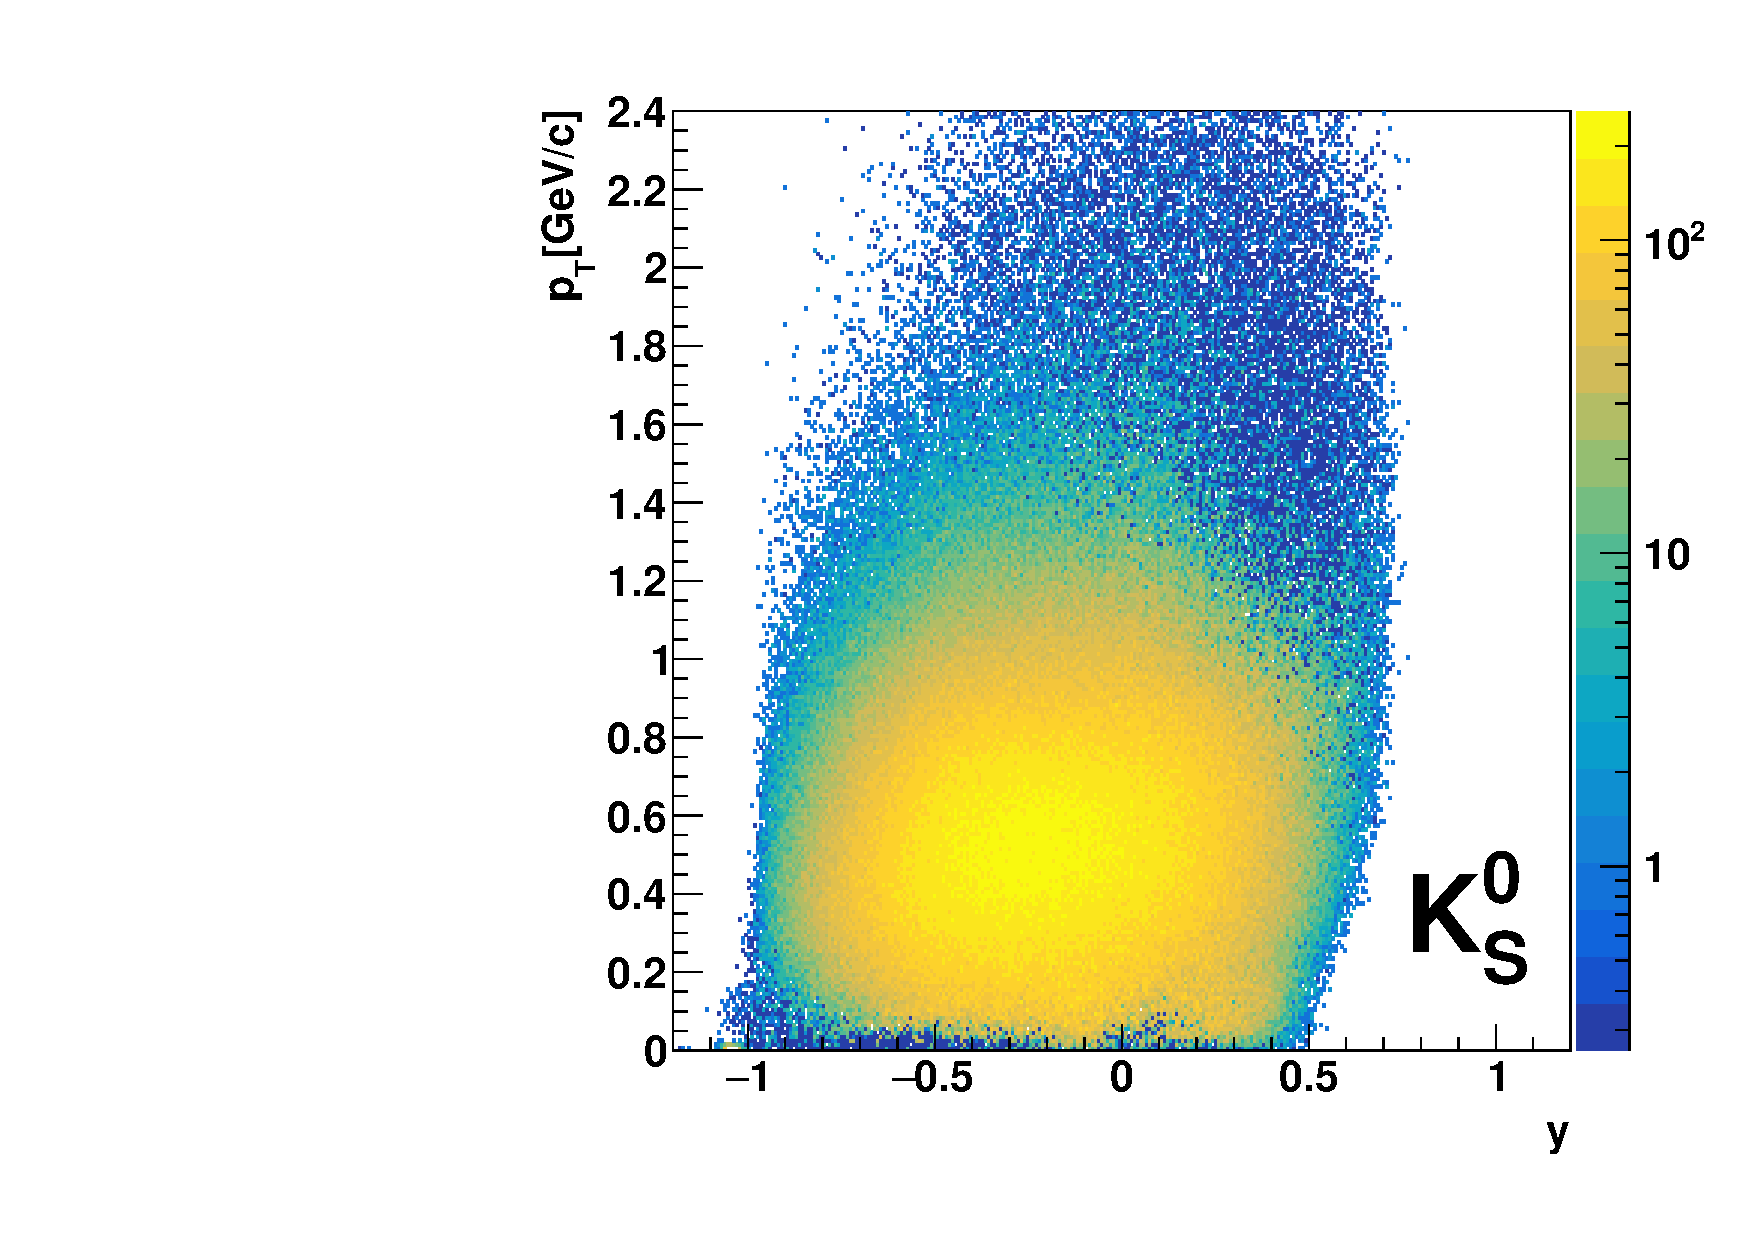
\includegraphics[width=0.49\linewidth]{chapterX/fig/ks_acceptance_v15.pdf}
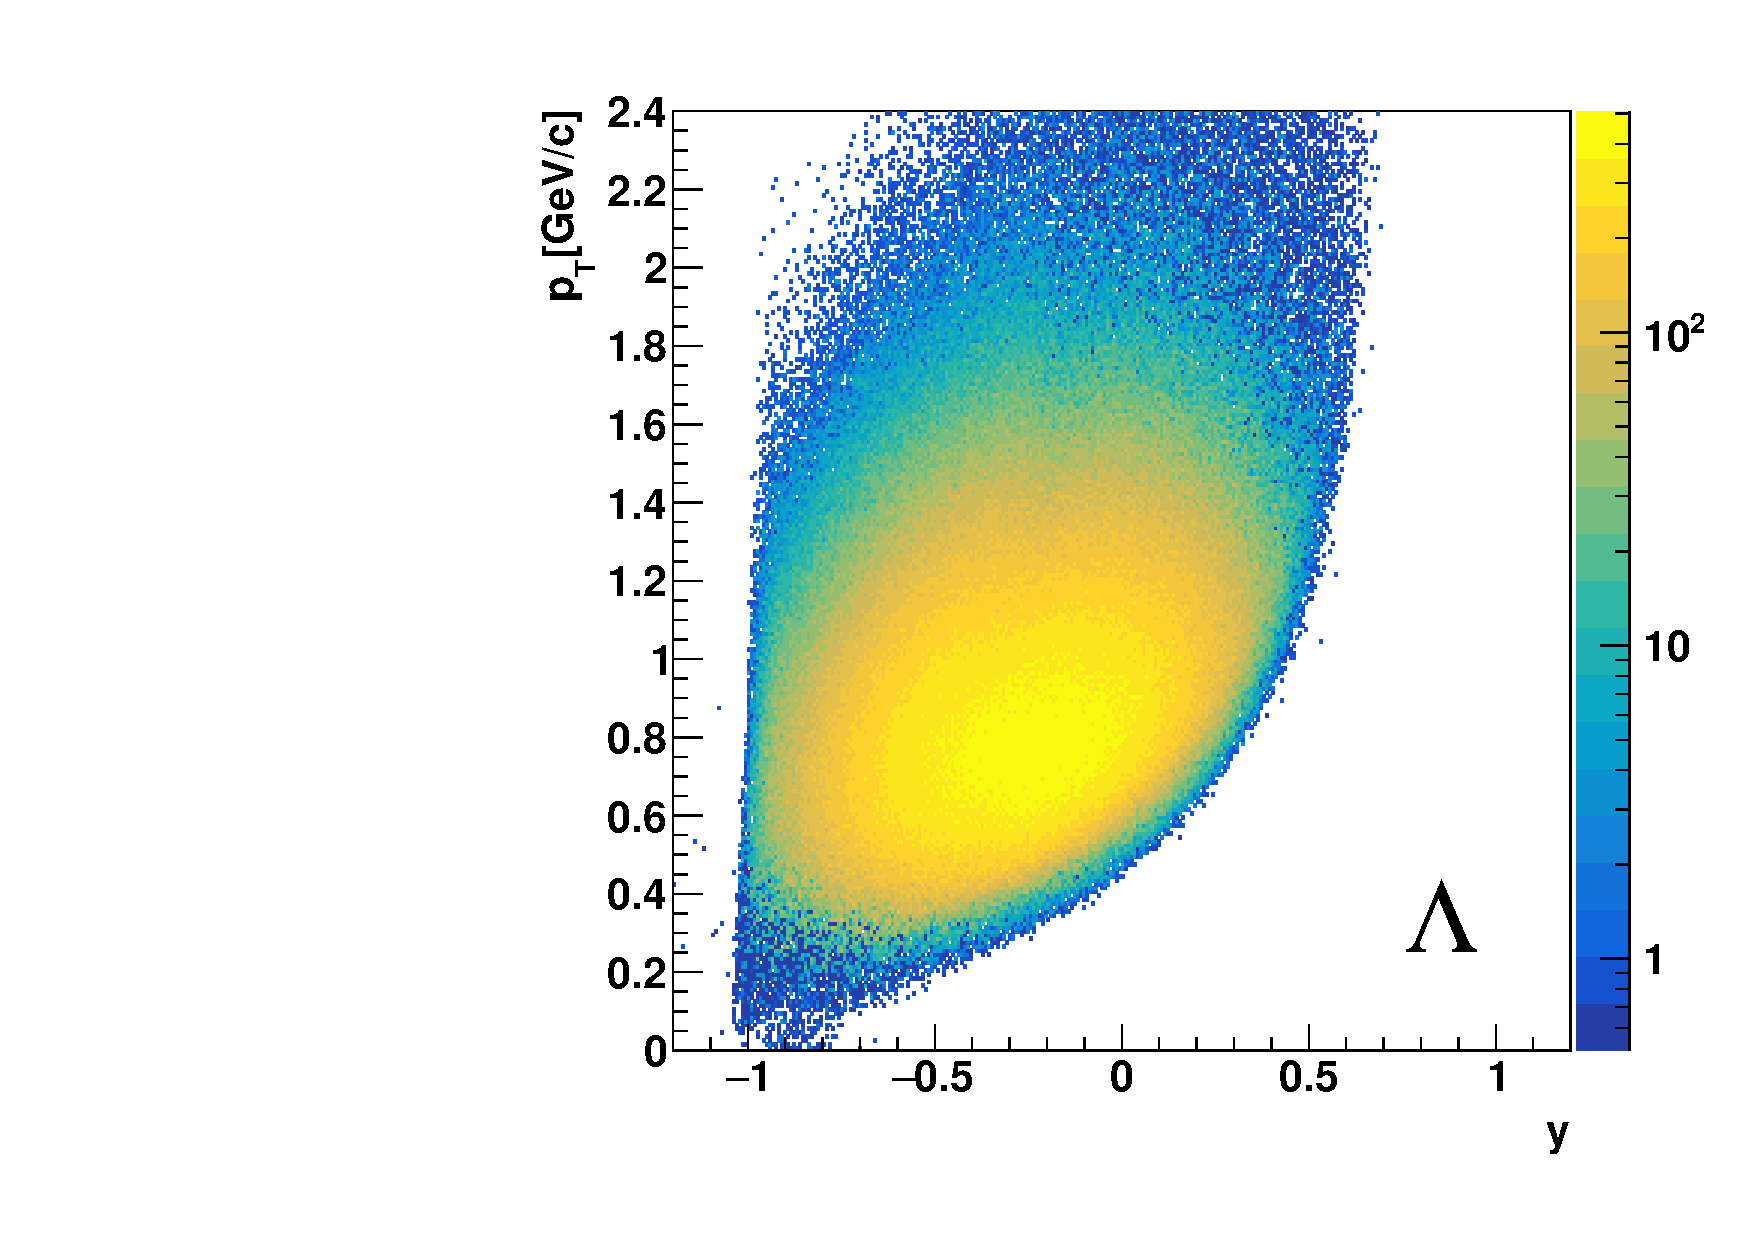
\includegraphics[width=0.49\linewidth]{chapterX/fig/ld_acceptance_v15.pdf}
\caption{Acceptance of $K^0_S$(left) and $\Lambda$(right) for $10-40\%$ centrality at $\sqrt{s_{NN}}$ = 3 GeV.}
\label{ldks_acceptance}
\end{figure}



\subsubsection{Efficiency corrections}

\begin{figure}[h]
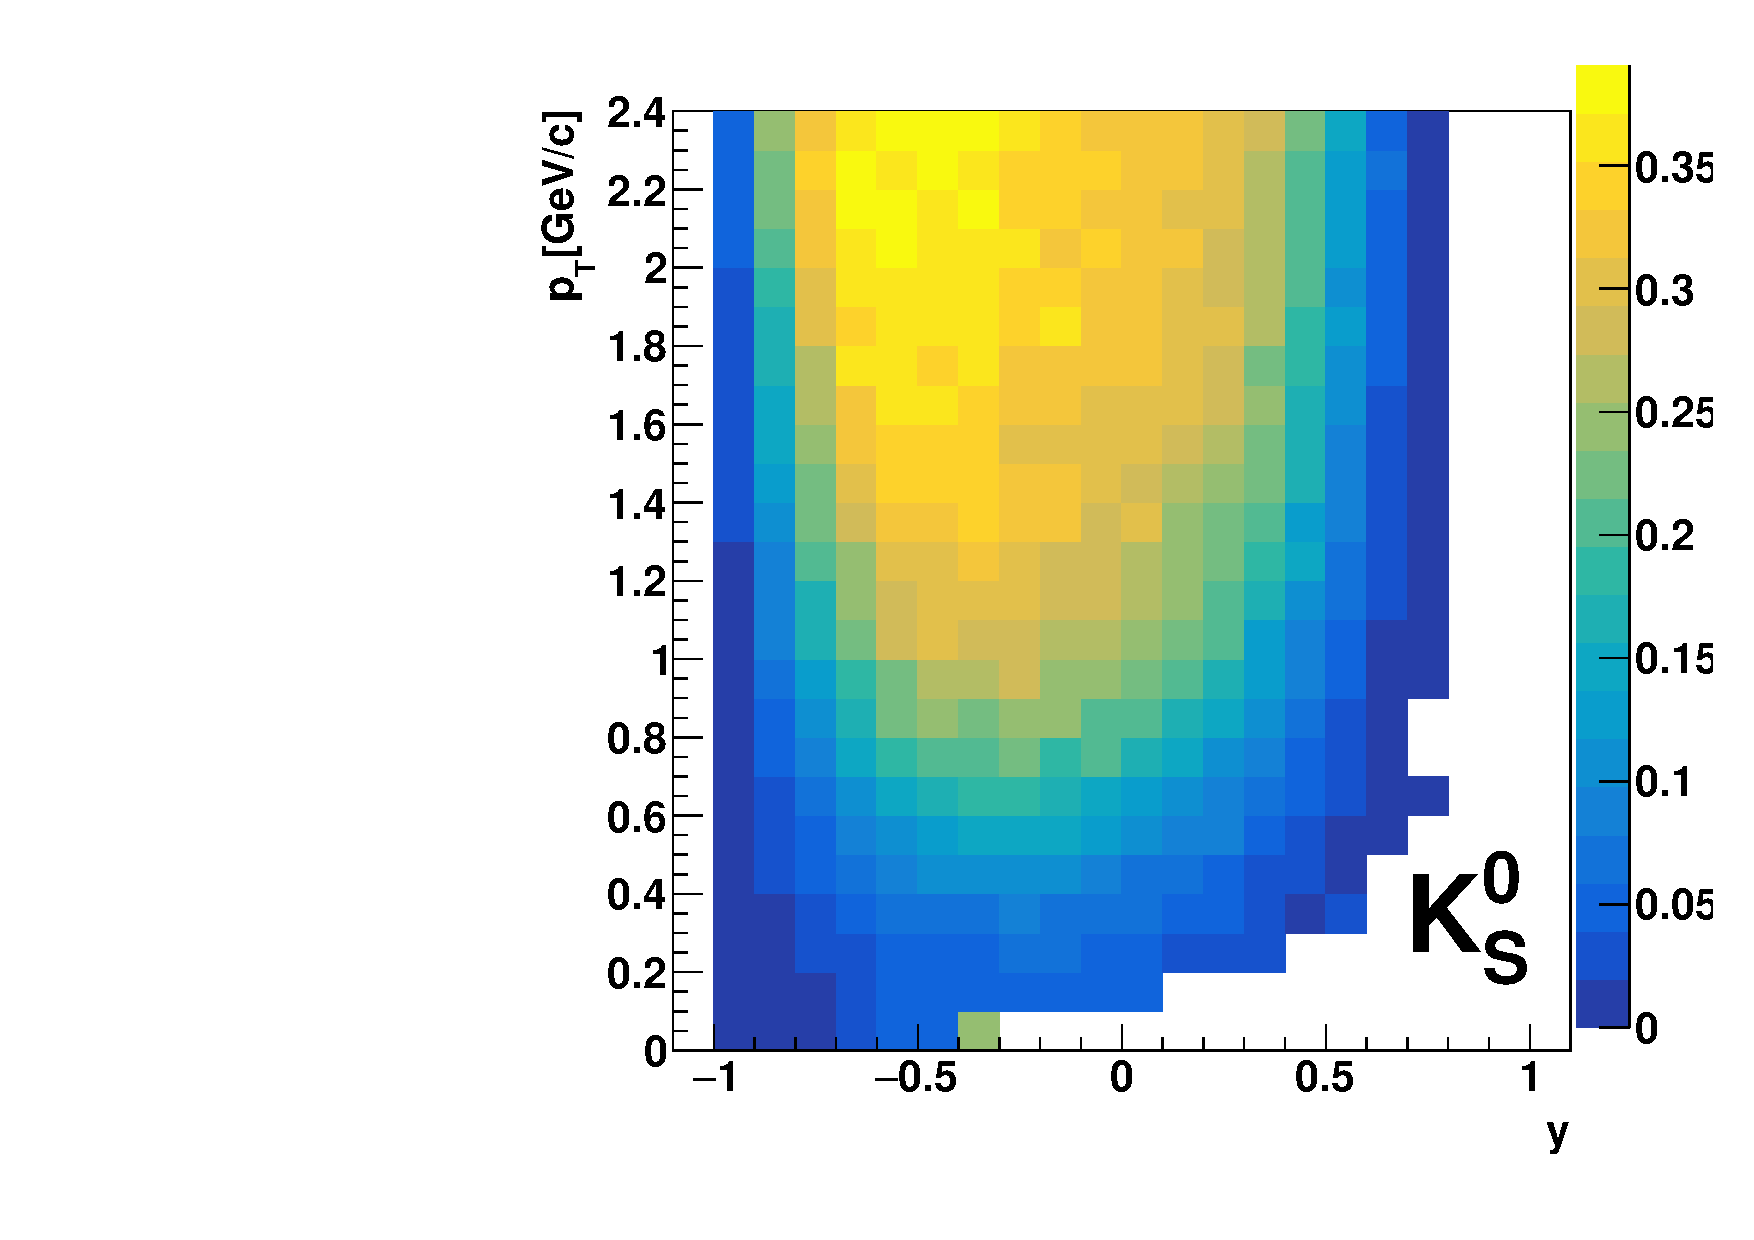
\includegraphics[width=0.49\linewidth]{chapterX/fig/ks_efficiency_v15.pdf}
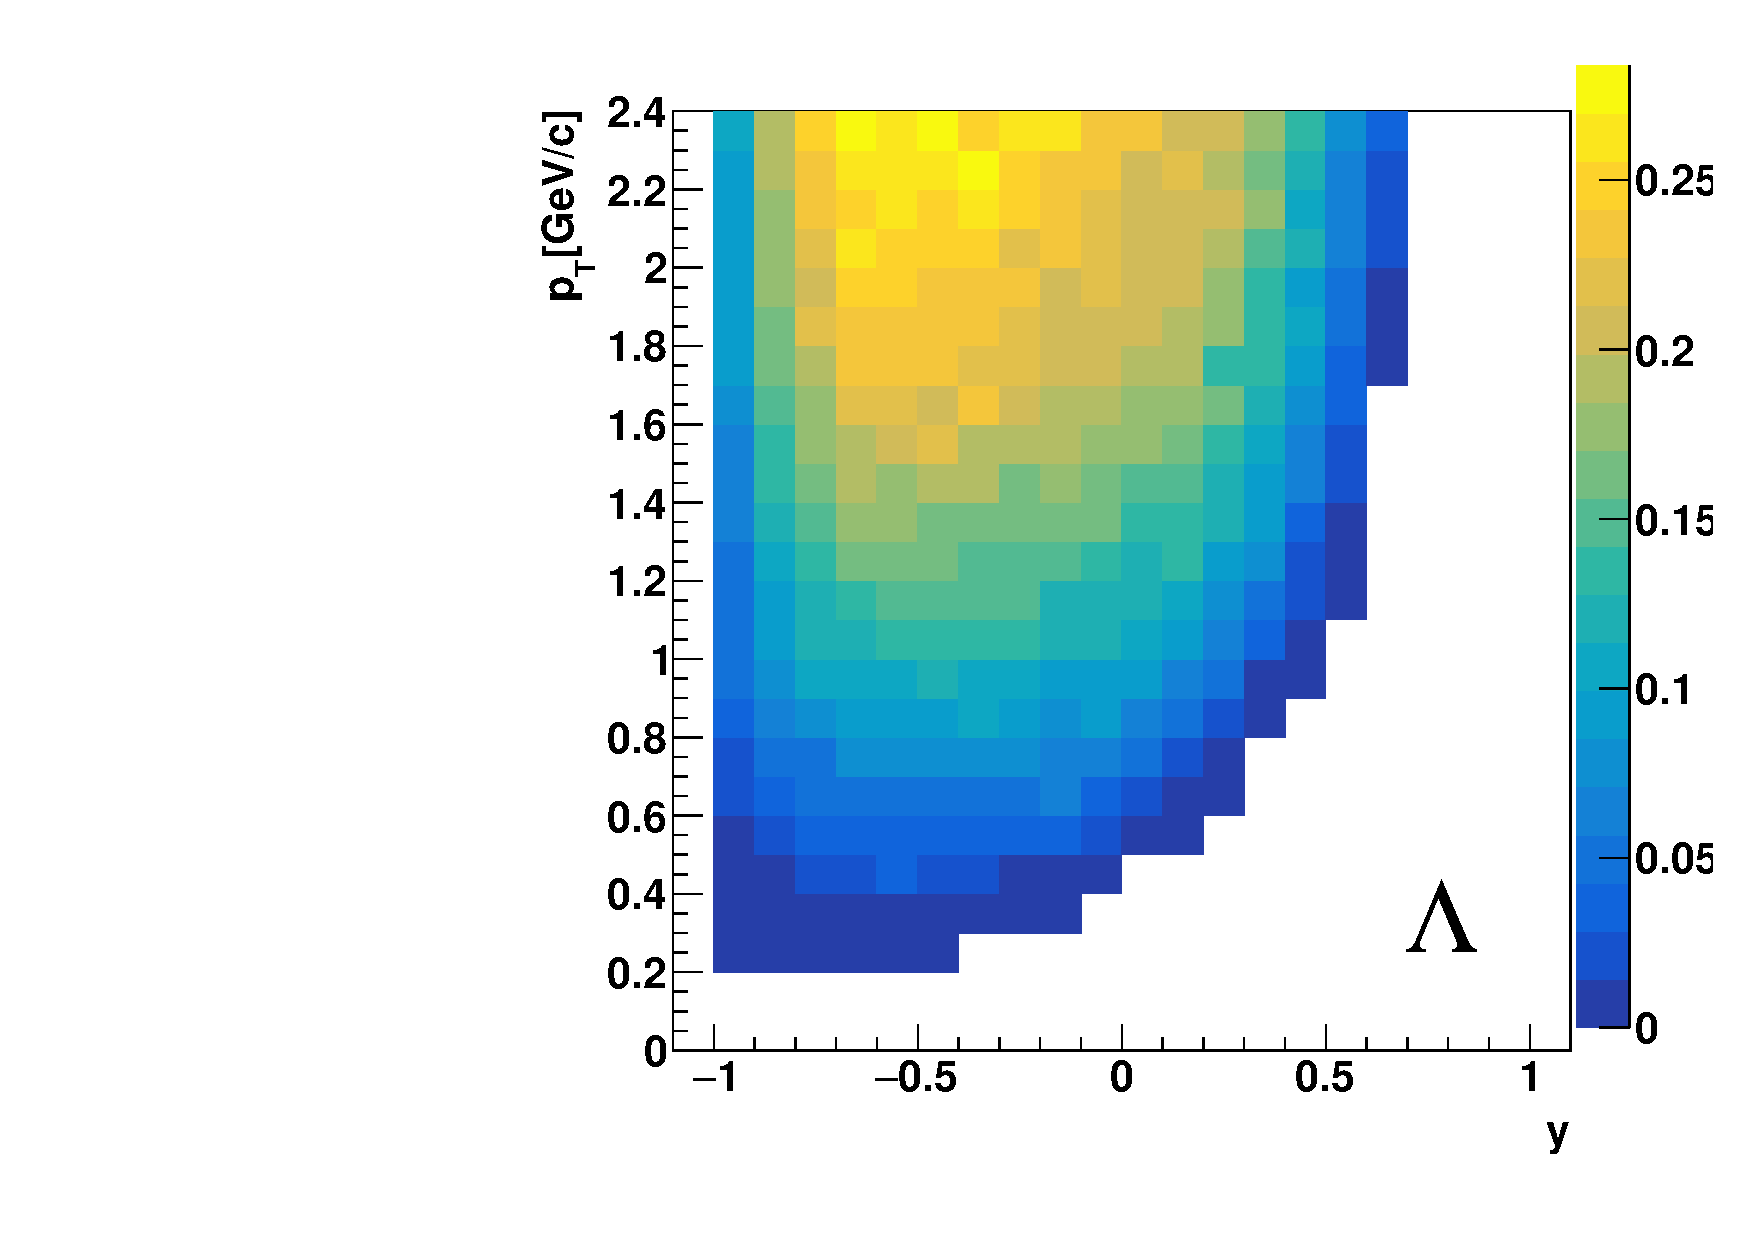
\includegraphics[width=0.49\linewidth]{chapterX/fig/ld_efficiency_v15.pdf}
\caption{Reconstruction efficiency of $K^0_S$(left) and $\Lambda$(right), as a function of $y$ and $p_{\rm{T}}$ for $10-40\%$ centrality at $\sqrt{s_{NN}}$ = 3 GeV.}
\label{ldks_acceptance}
\end{figure}


\subsection{$v_1$ and $v_2$ extraction}
\subsection{Systematic uncertainties}
\subsubsection{$v_1$}

\begin{figure}[h]
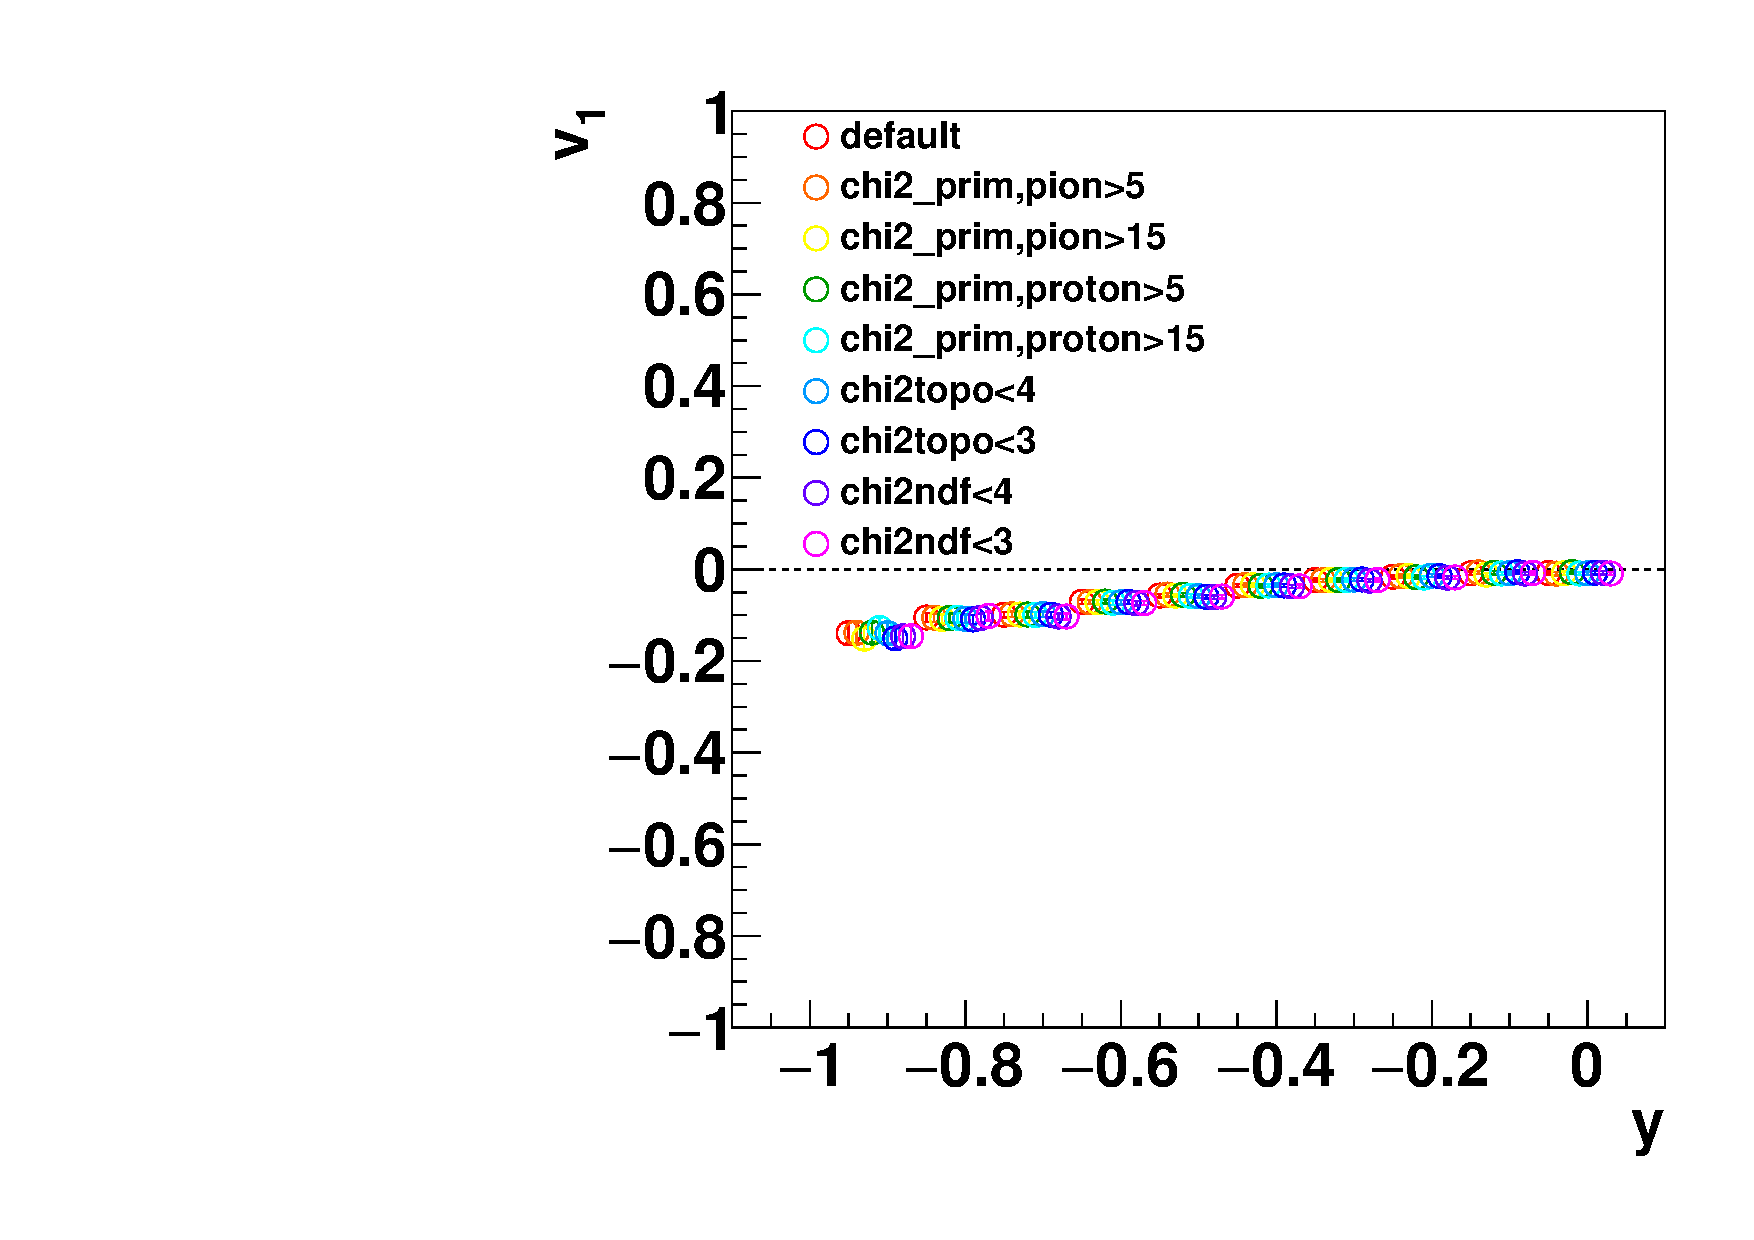
\includegraphics[width=0.49\linewidth]{chapterX/fig/ks_sys_cut_v1.pdf}
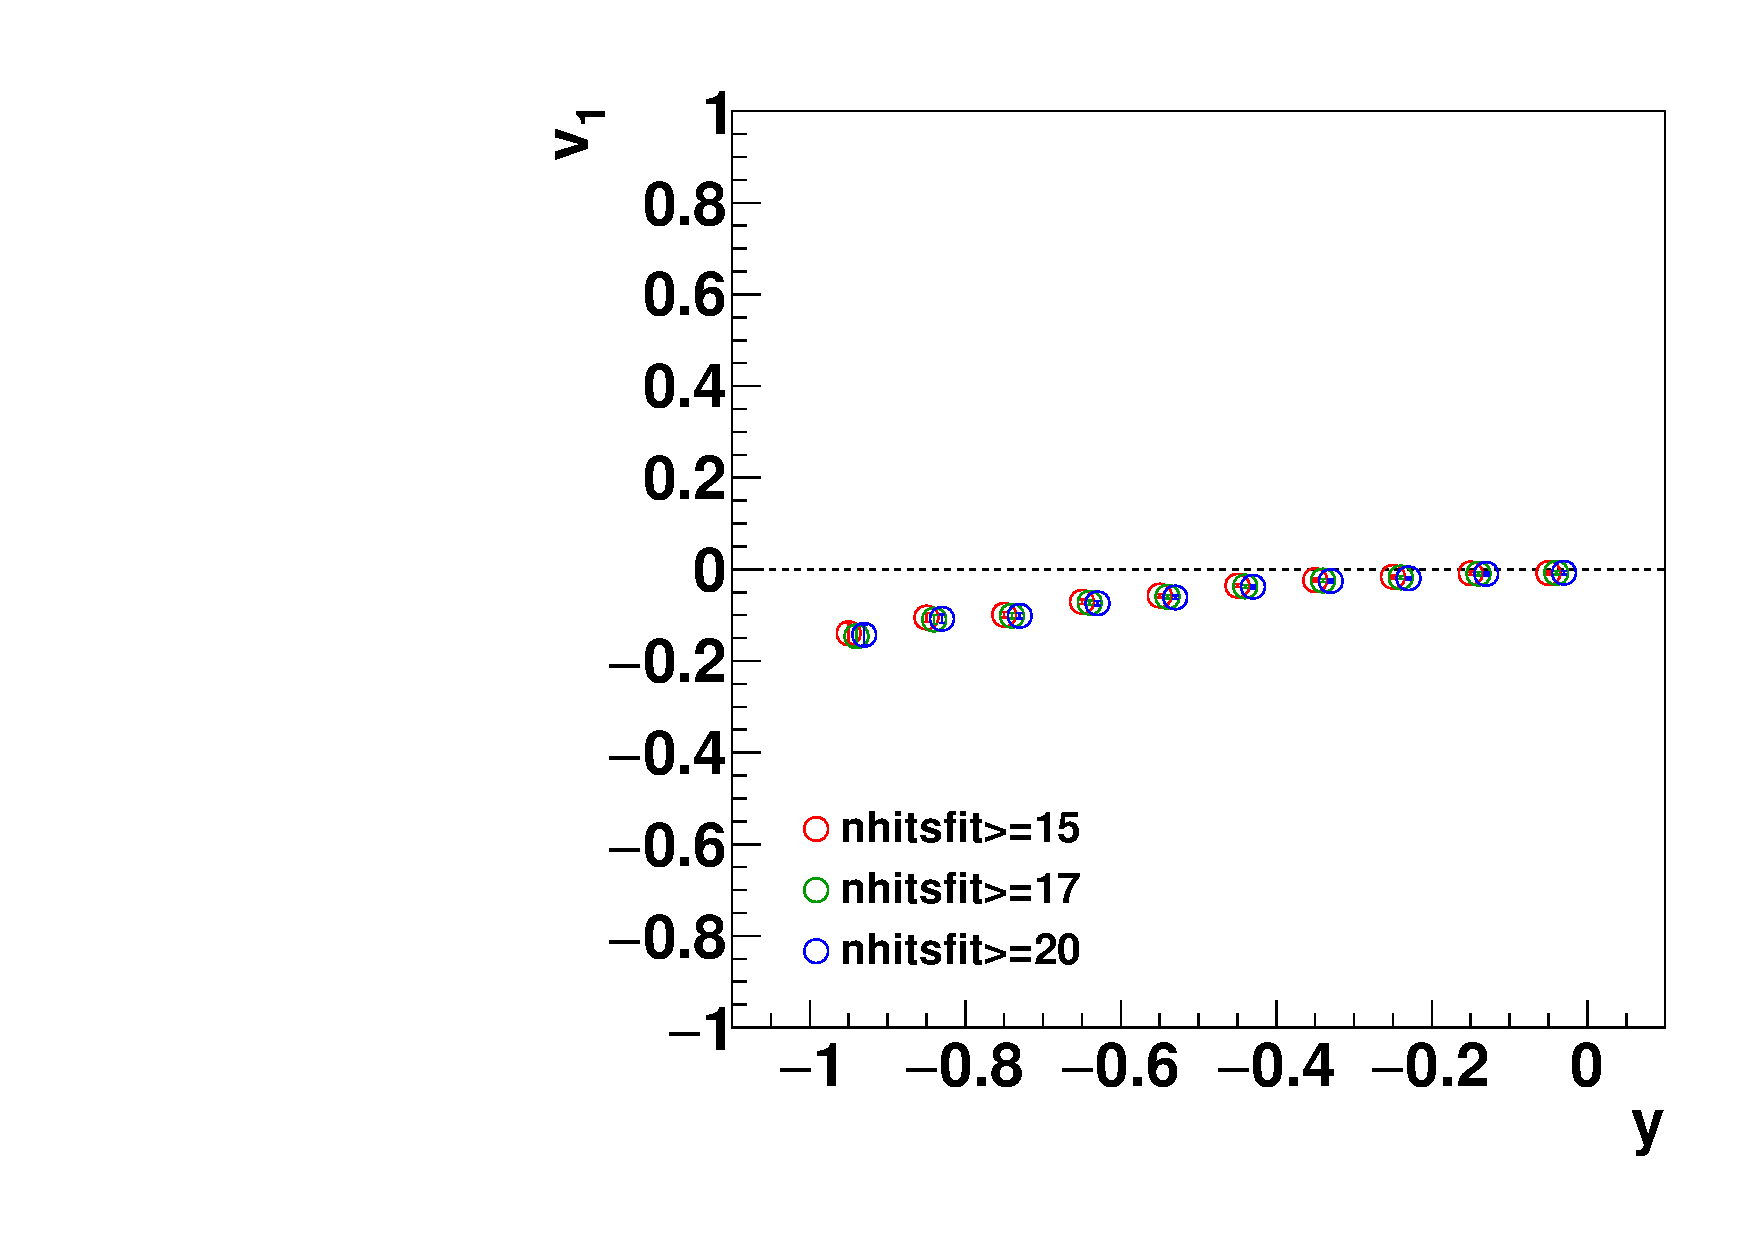
\includegraphics[width=0.49\linewidth]{chapterX/fig/ks_sys_cut_v1_nhits.pdf}
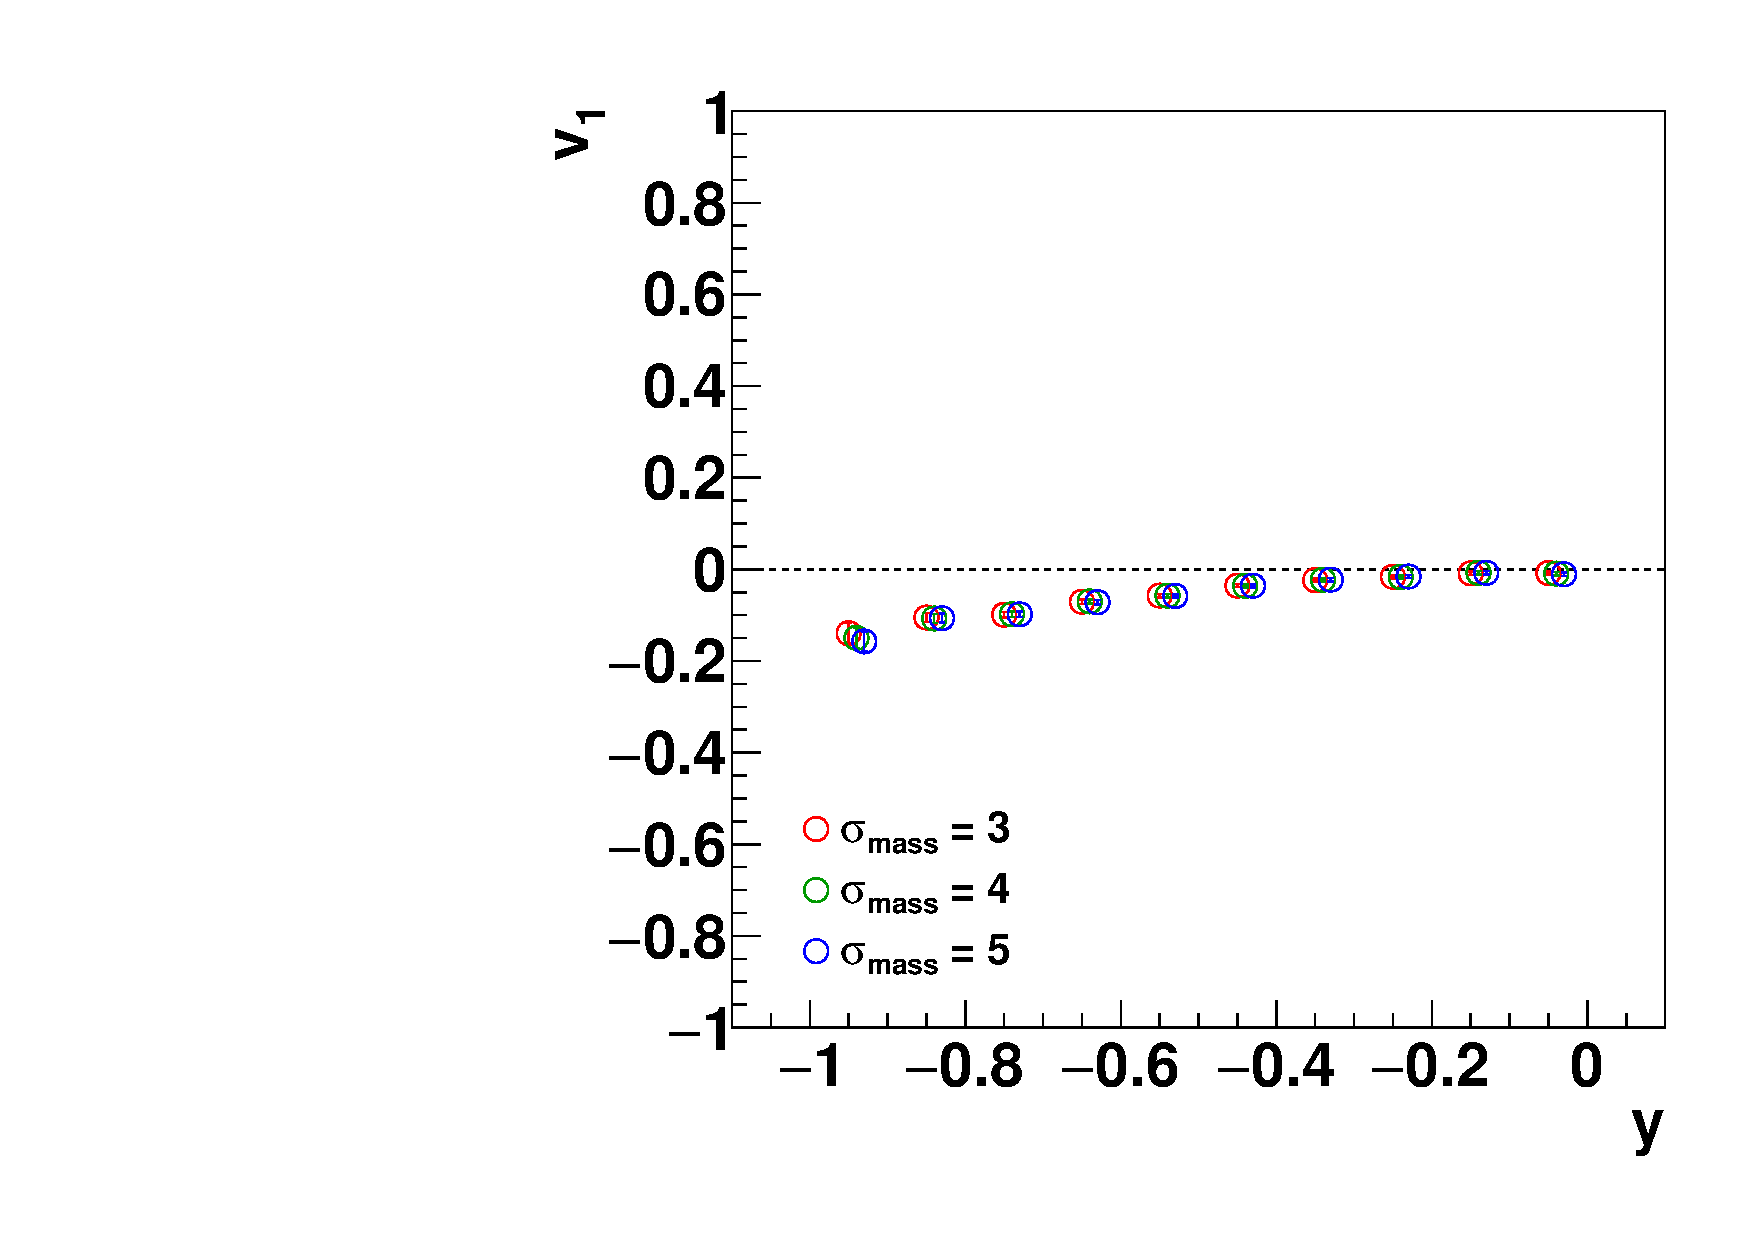
\includegraphics[width=0.49\linewidth]{FXT3gev/chapterX/fig/ks_sys_cut_v1_msigma.pdf}
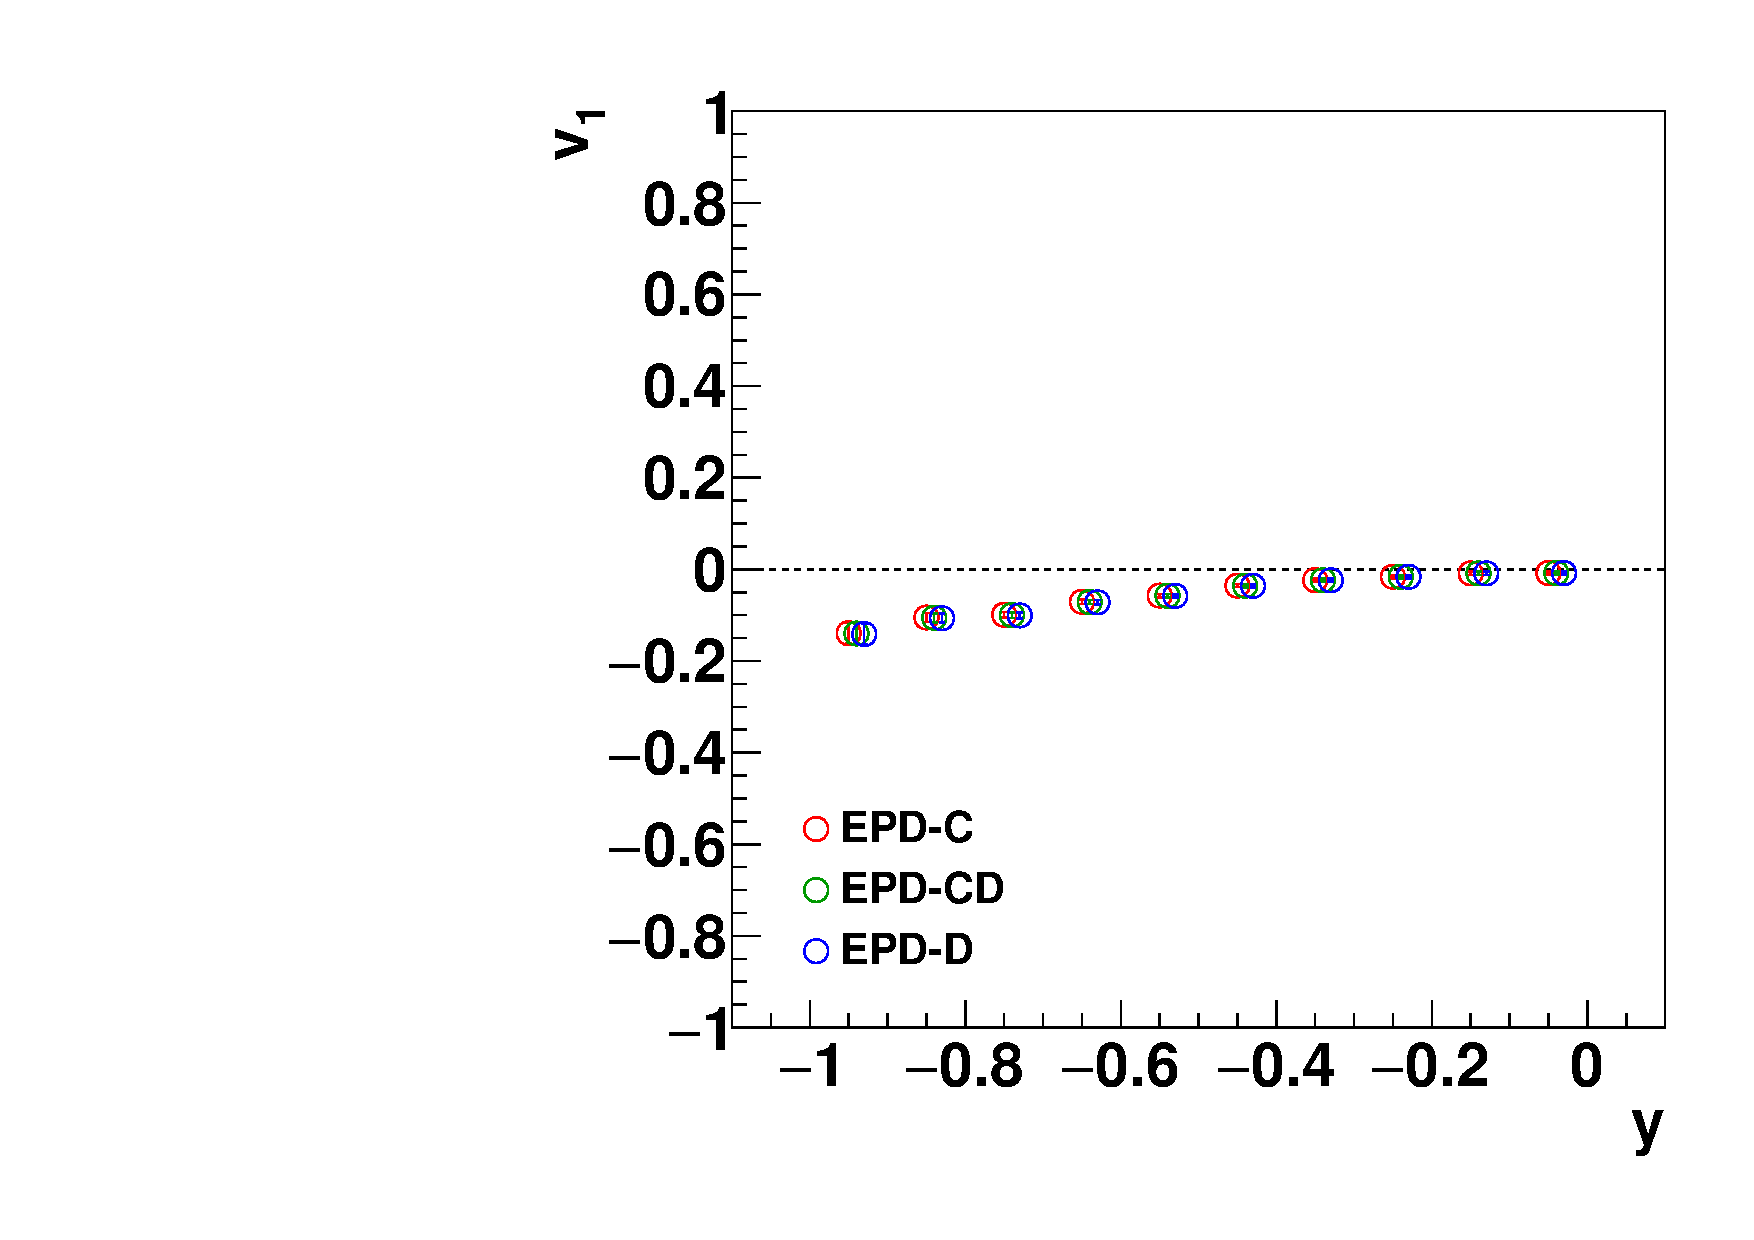
\includegraphics[width=0.49\linewidth]{FXT3gev/chapterX/fig/ks_sys_cut_v1_epdres.pdf}
\caption{Systematic uncertainty study for $v_{1}$ as a function of rapidity in 10-40\% for $K^0_S$ at $\sqrt{s_{NN}}$ = 3 GeV.}
\label{ks_v1y_sys}
\end{figure}

\begin{figure}[h]
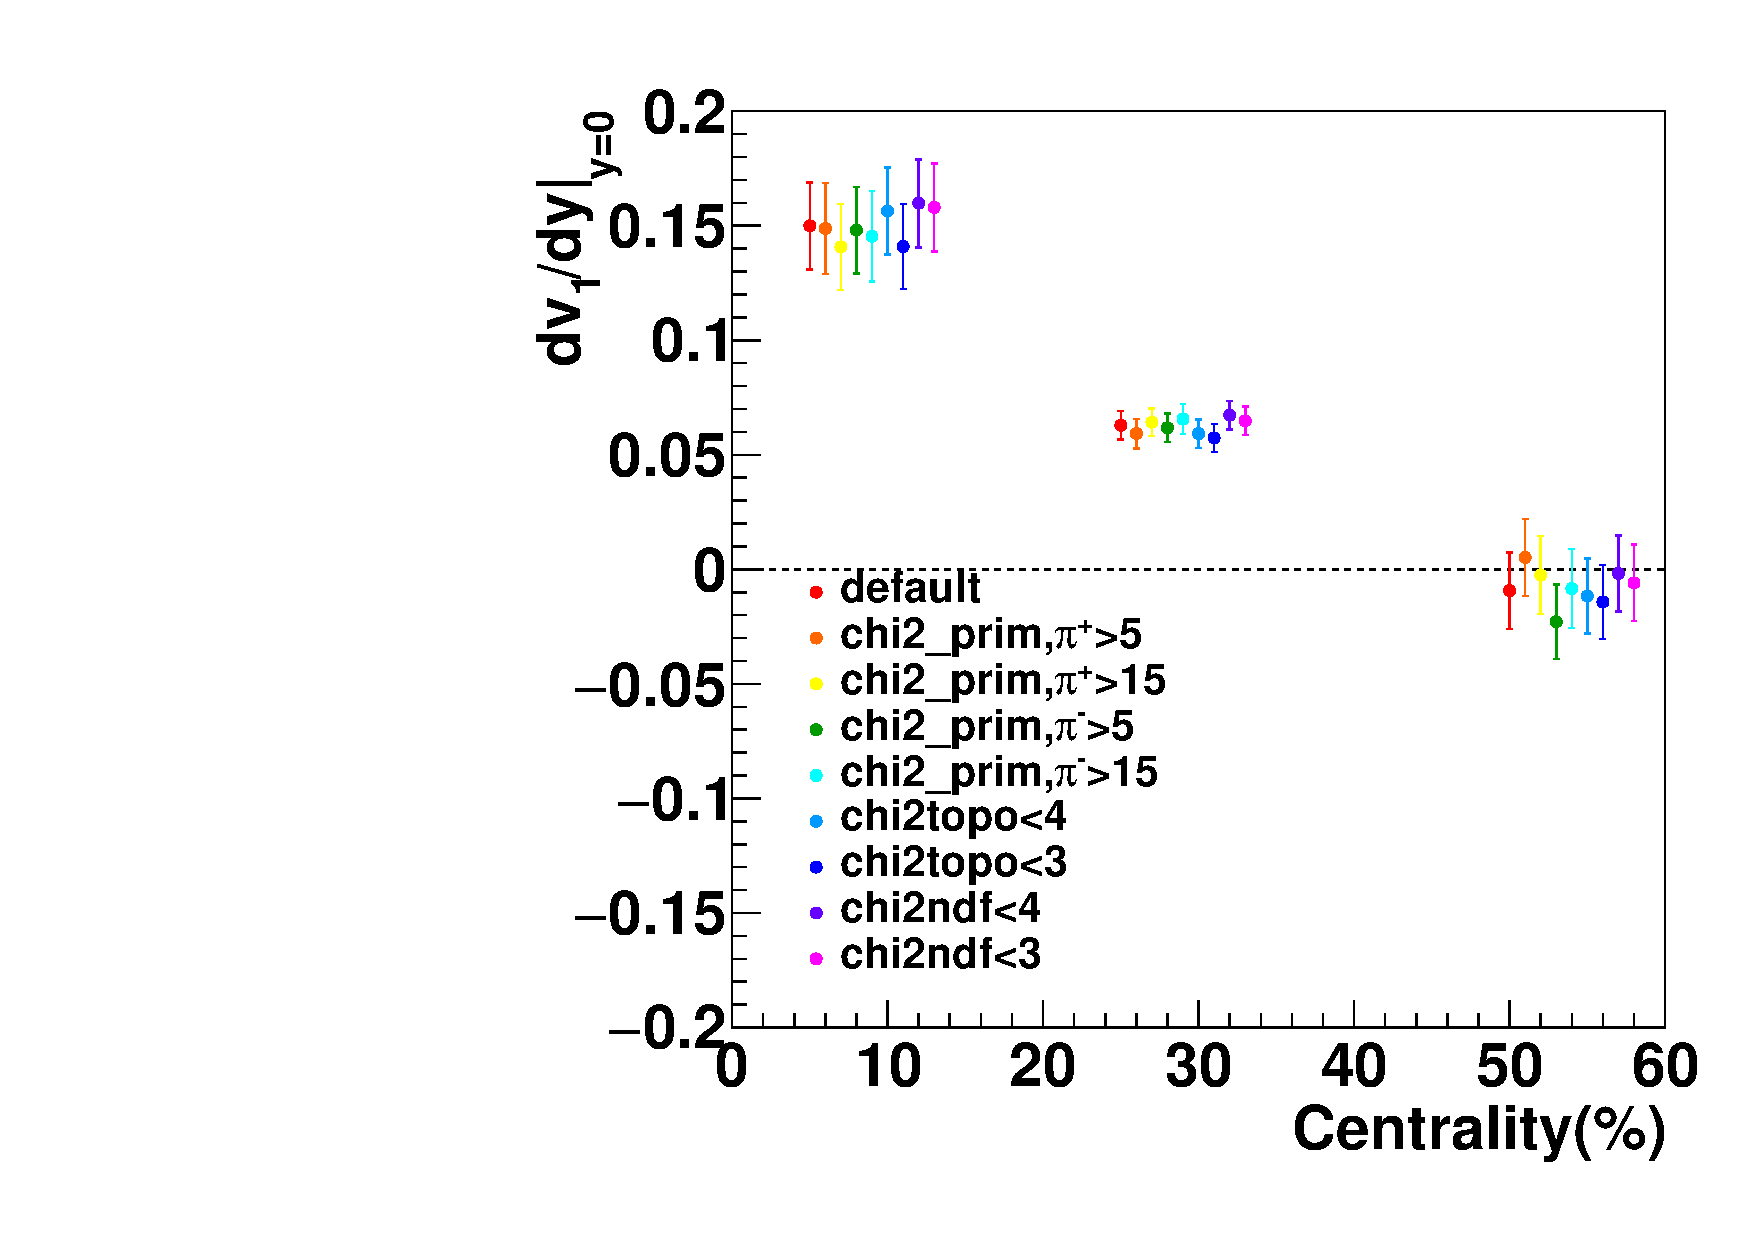
\includegraphics[width=0.49\linewidth]{chapterX/fig/ks_sys_cut_vn.pdf}
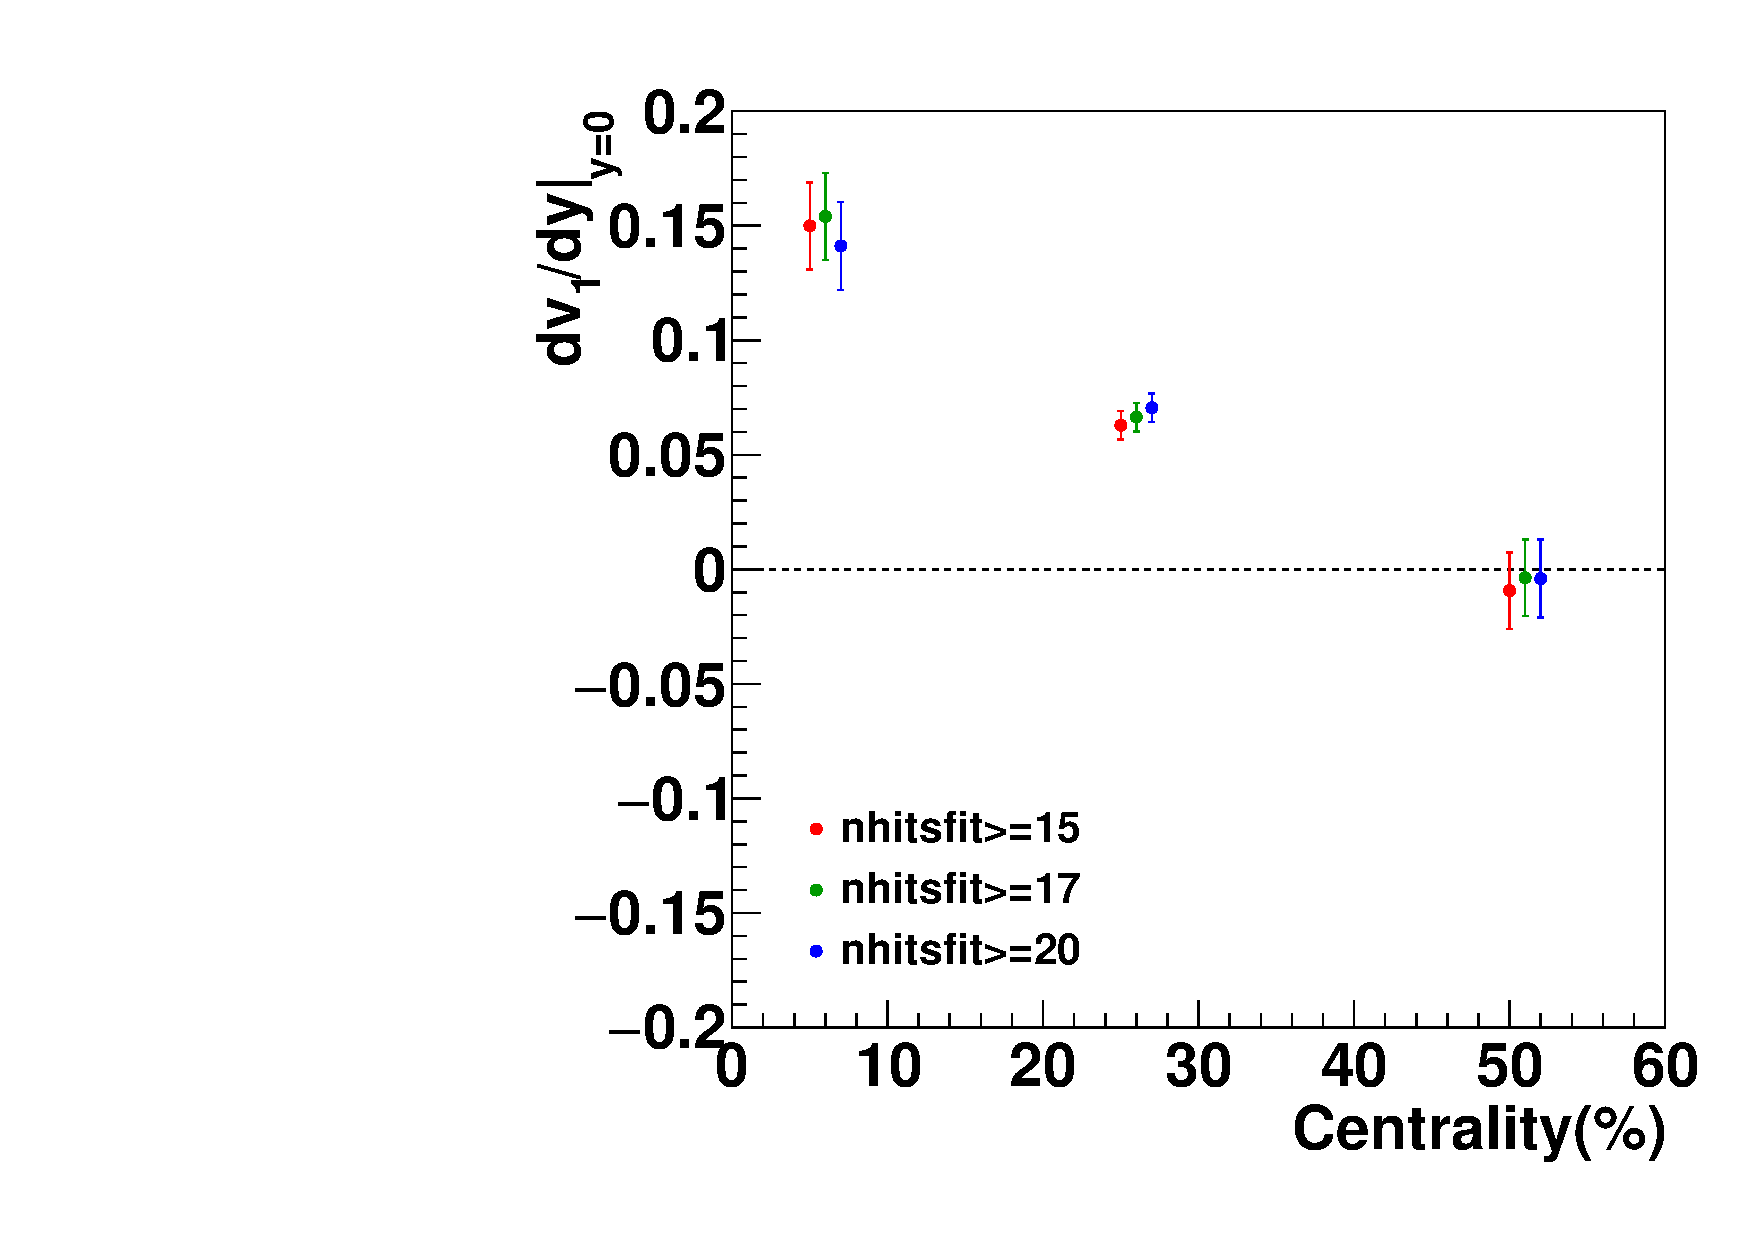
\includegraphics[width=0.49\linewidth]{chapterX/fig/ks_sys_cut_vn_nhits.pdf}
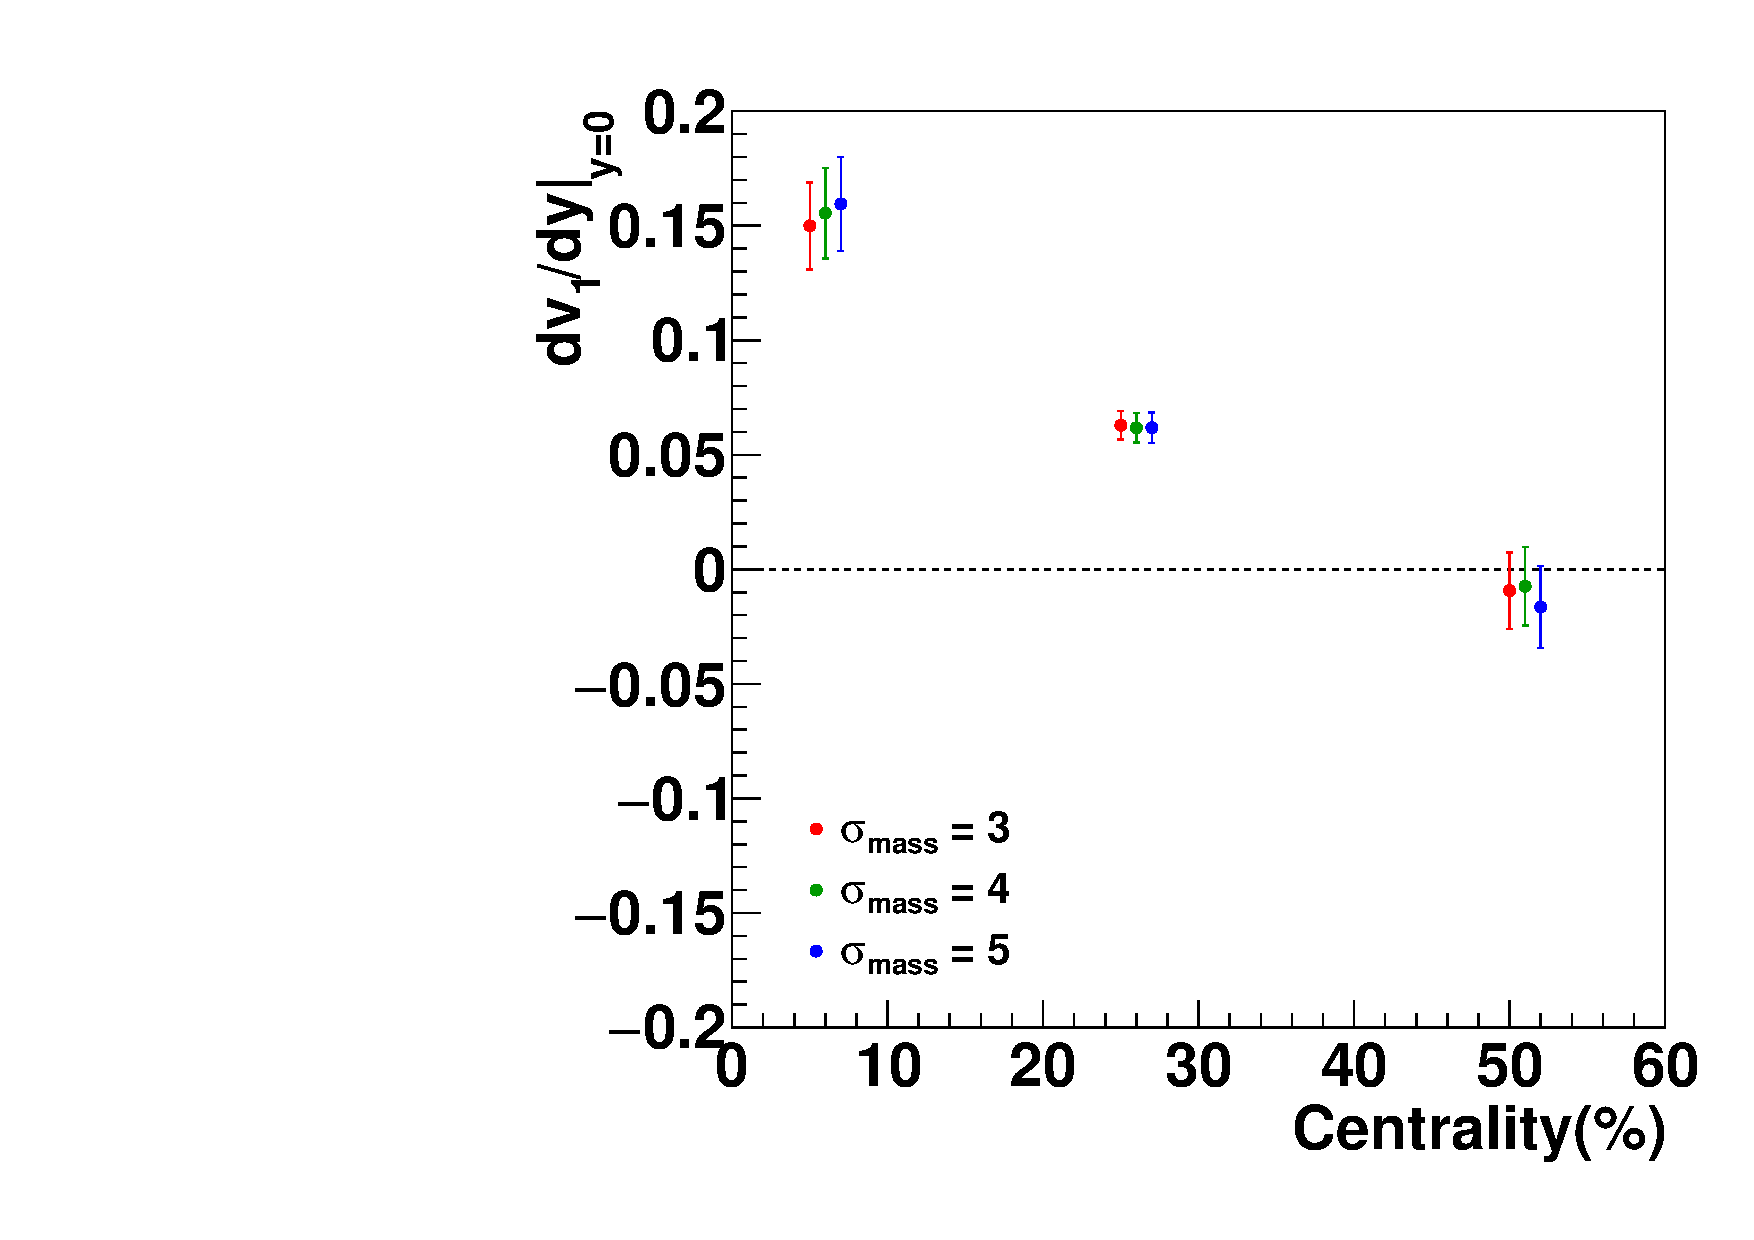
\includegraphics[width=0.49\linewidth]{FXT3gev/chapterX/fig/ks_sys_cut_vn_msigma.pdf}
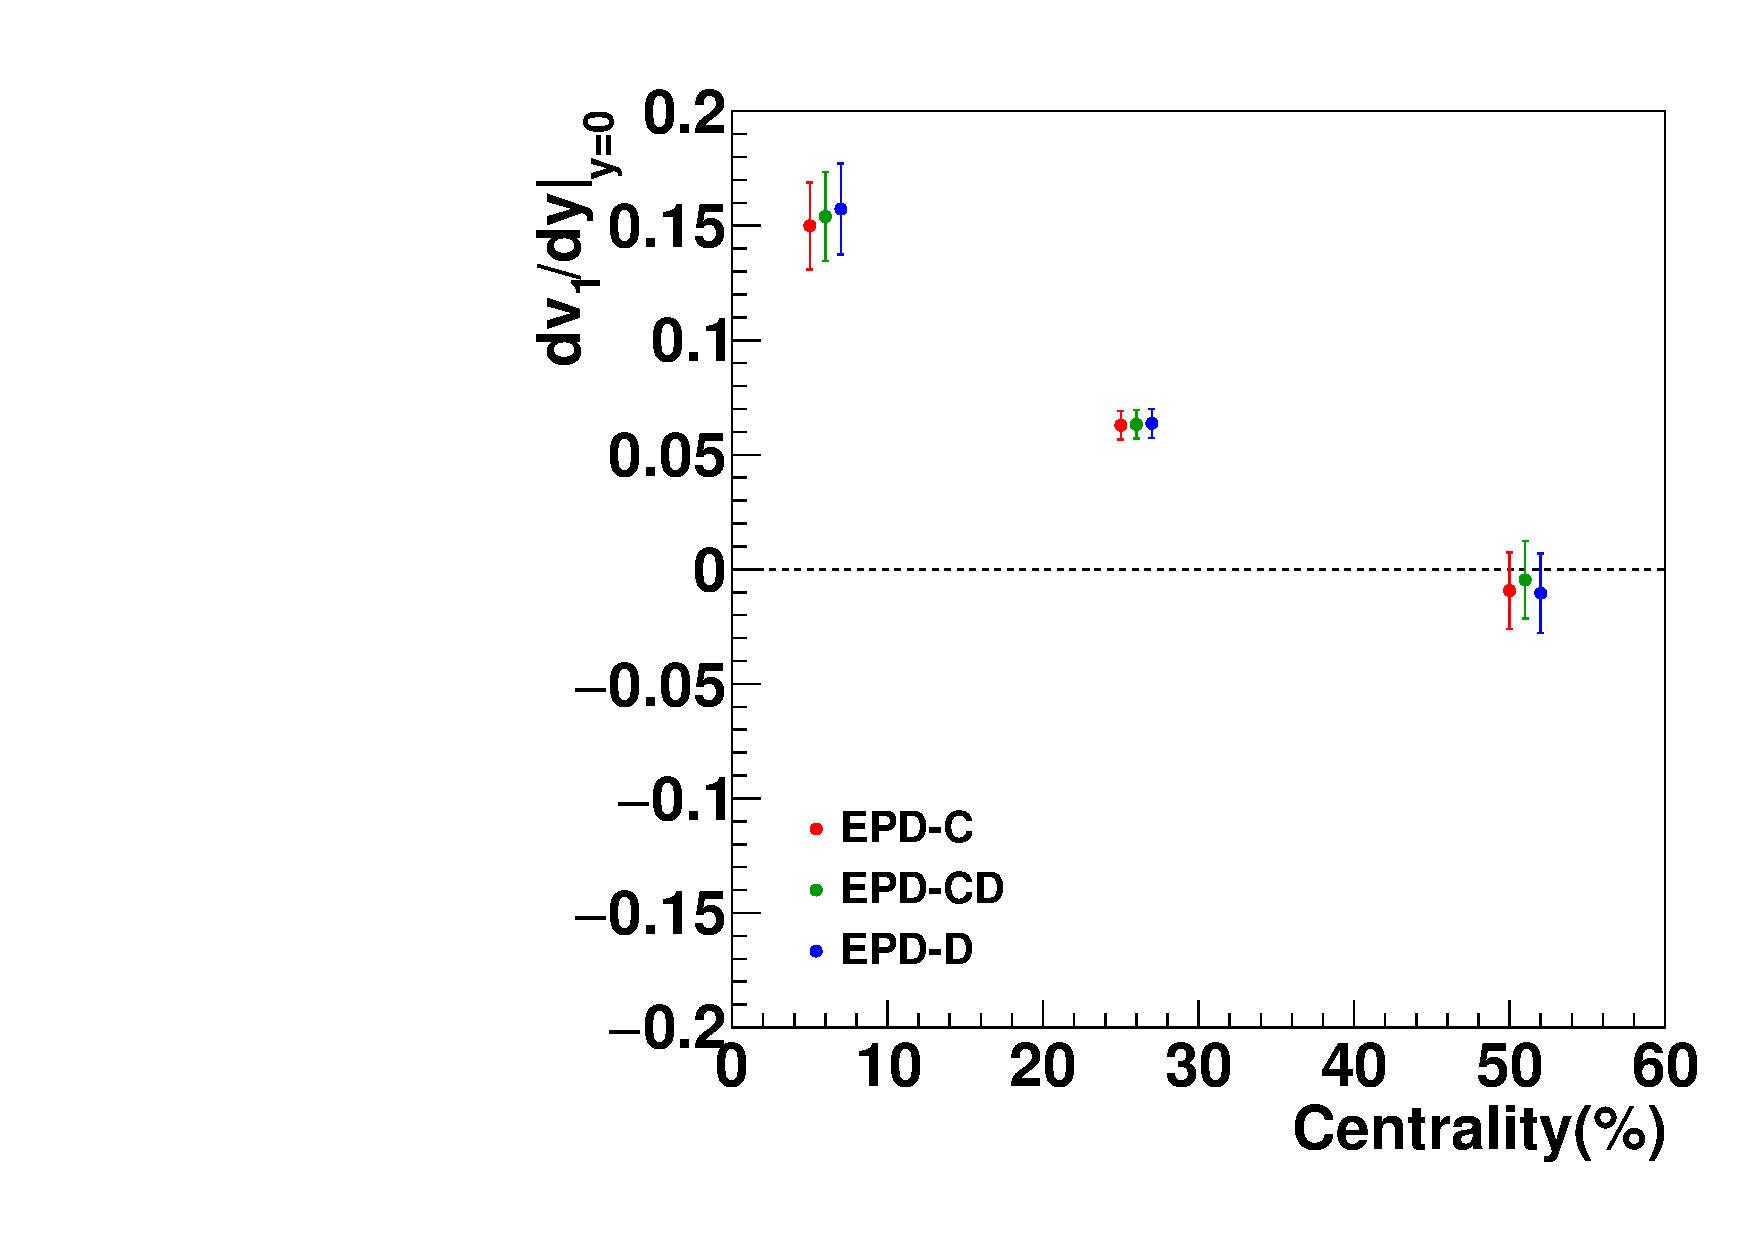
\includegraphics[width=0.49\linewidth]{FXT3gev/chapterX/fig/ks_sys_cut_vn_epdres.pdf}
\caption{Systematic uncertainty study for $dv_{1}/dy$ as a function of centrality for $K^0_S$ at $\sqrt{s_{NN}}$ = 3 GeV.}
\label{ks_dv1dy_sys}
\end{figure}

\begin{figure}[h]
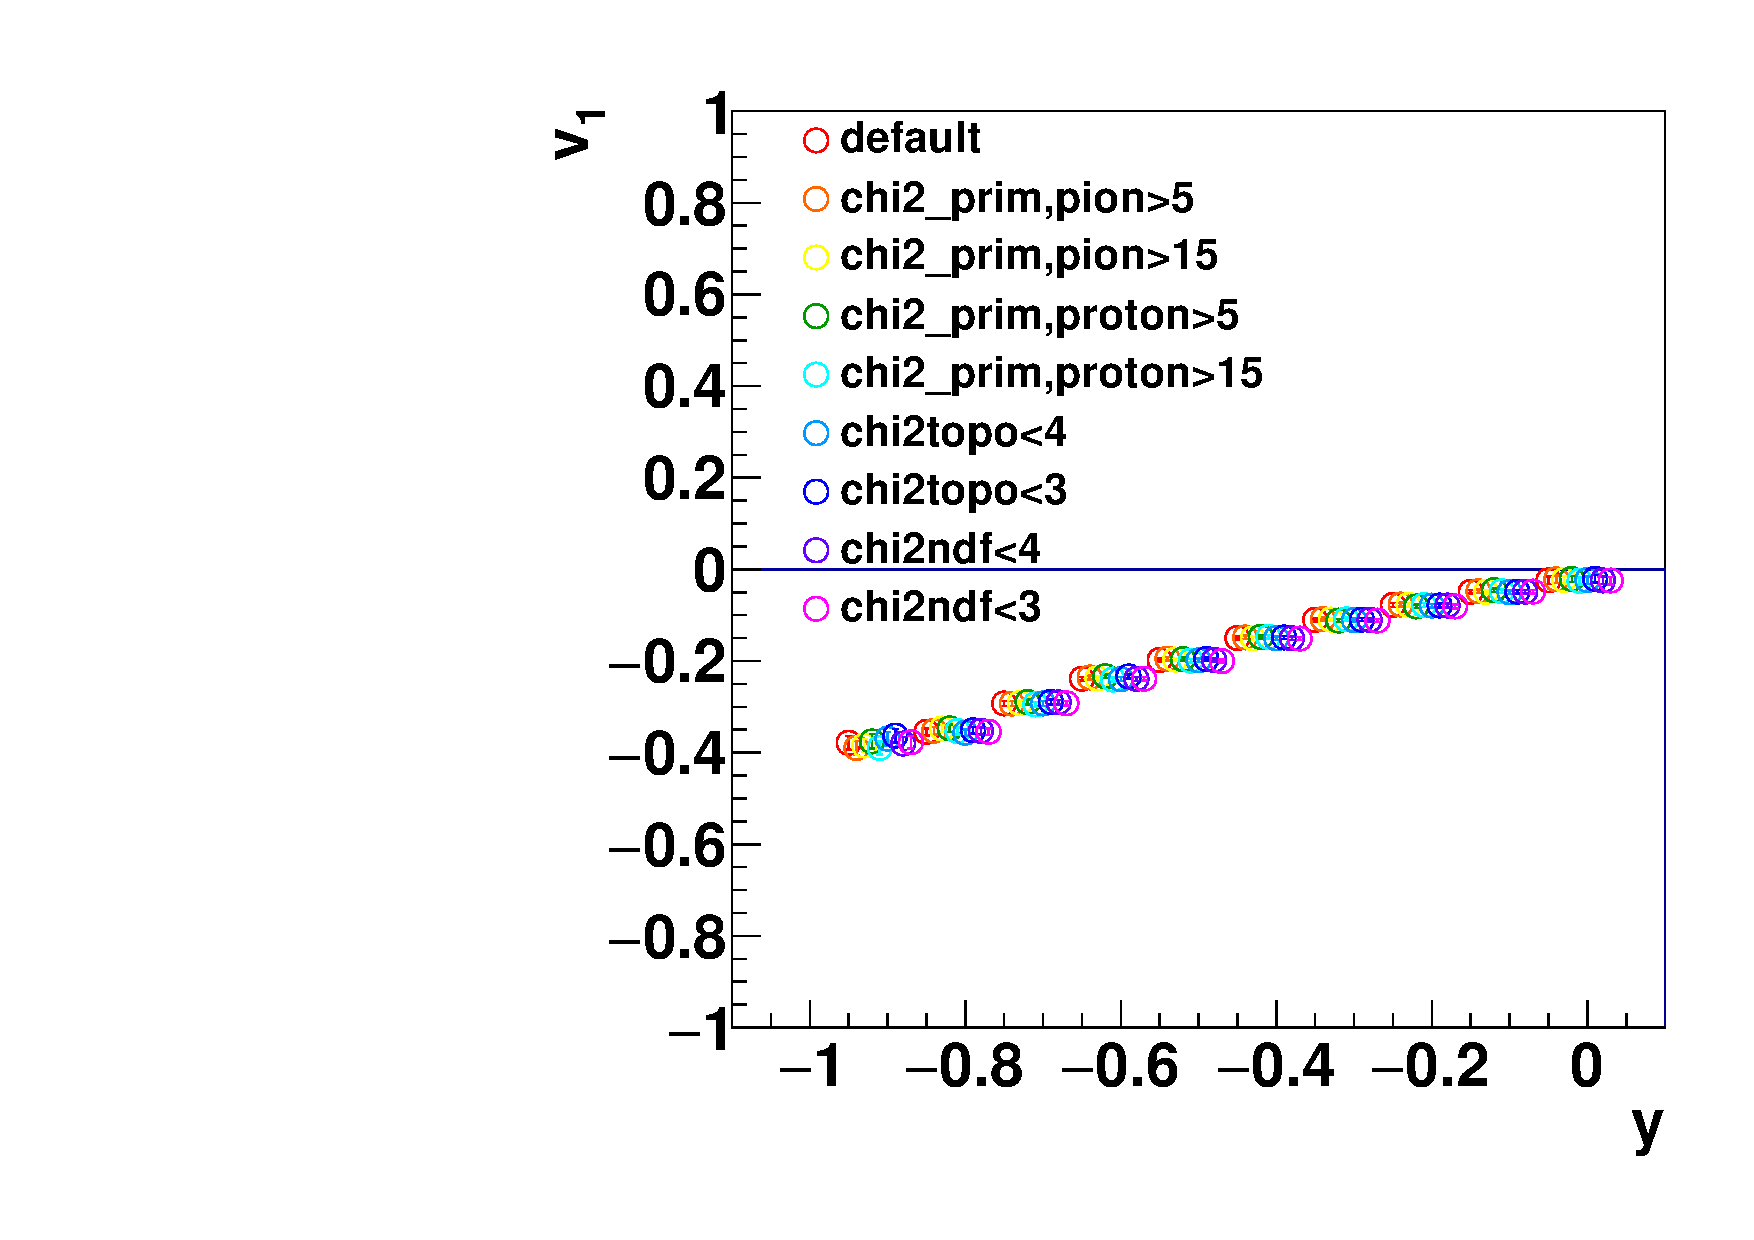
\includegraphics[width=0.49\linewidth]{chapterX/fig/ld_sys_cut_v1.pdf}
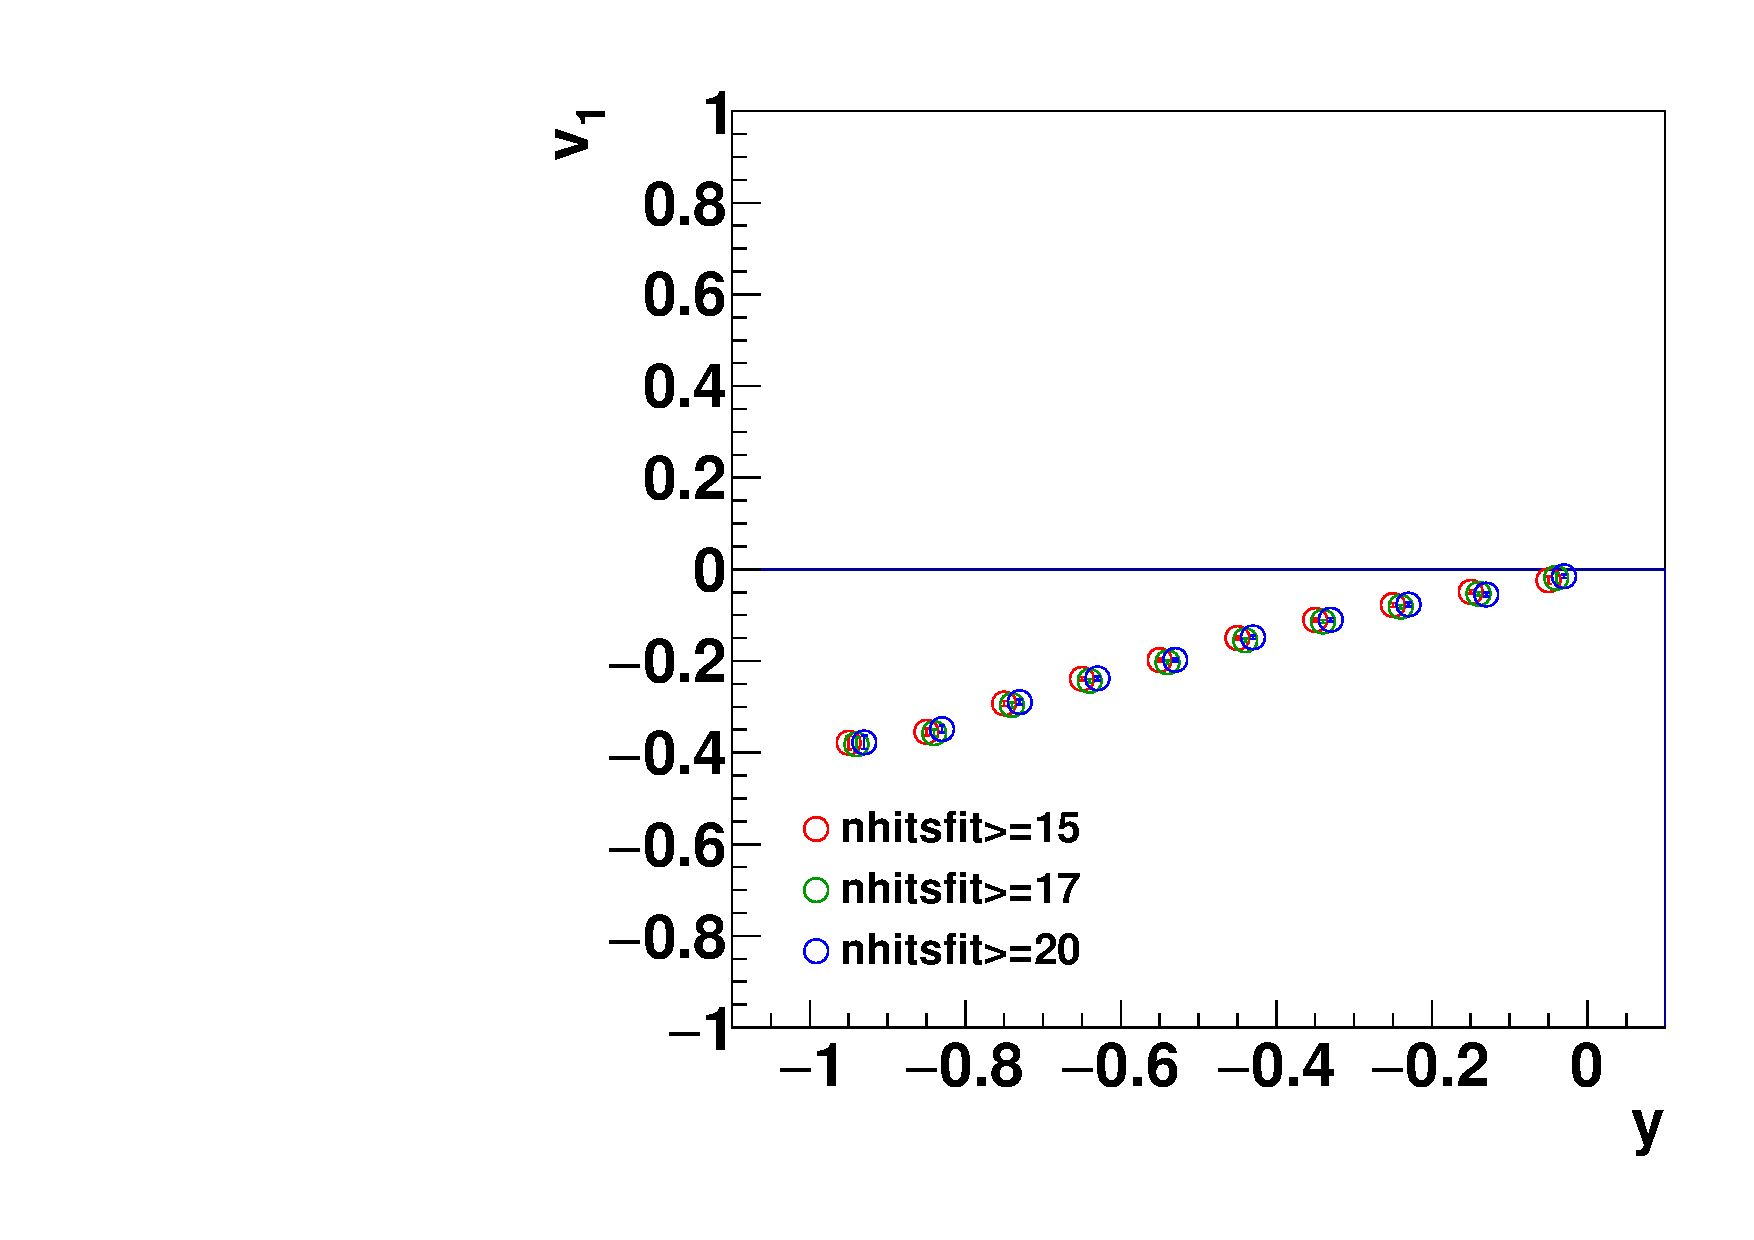
\includegraphics[width=0.49\linewidth]{chapterX/fig/ld_sys_cut_v1_nhits.pdf}
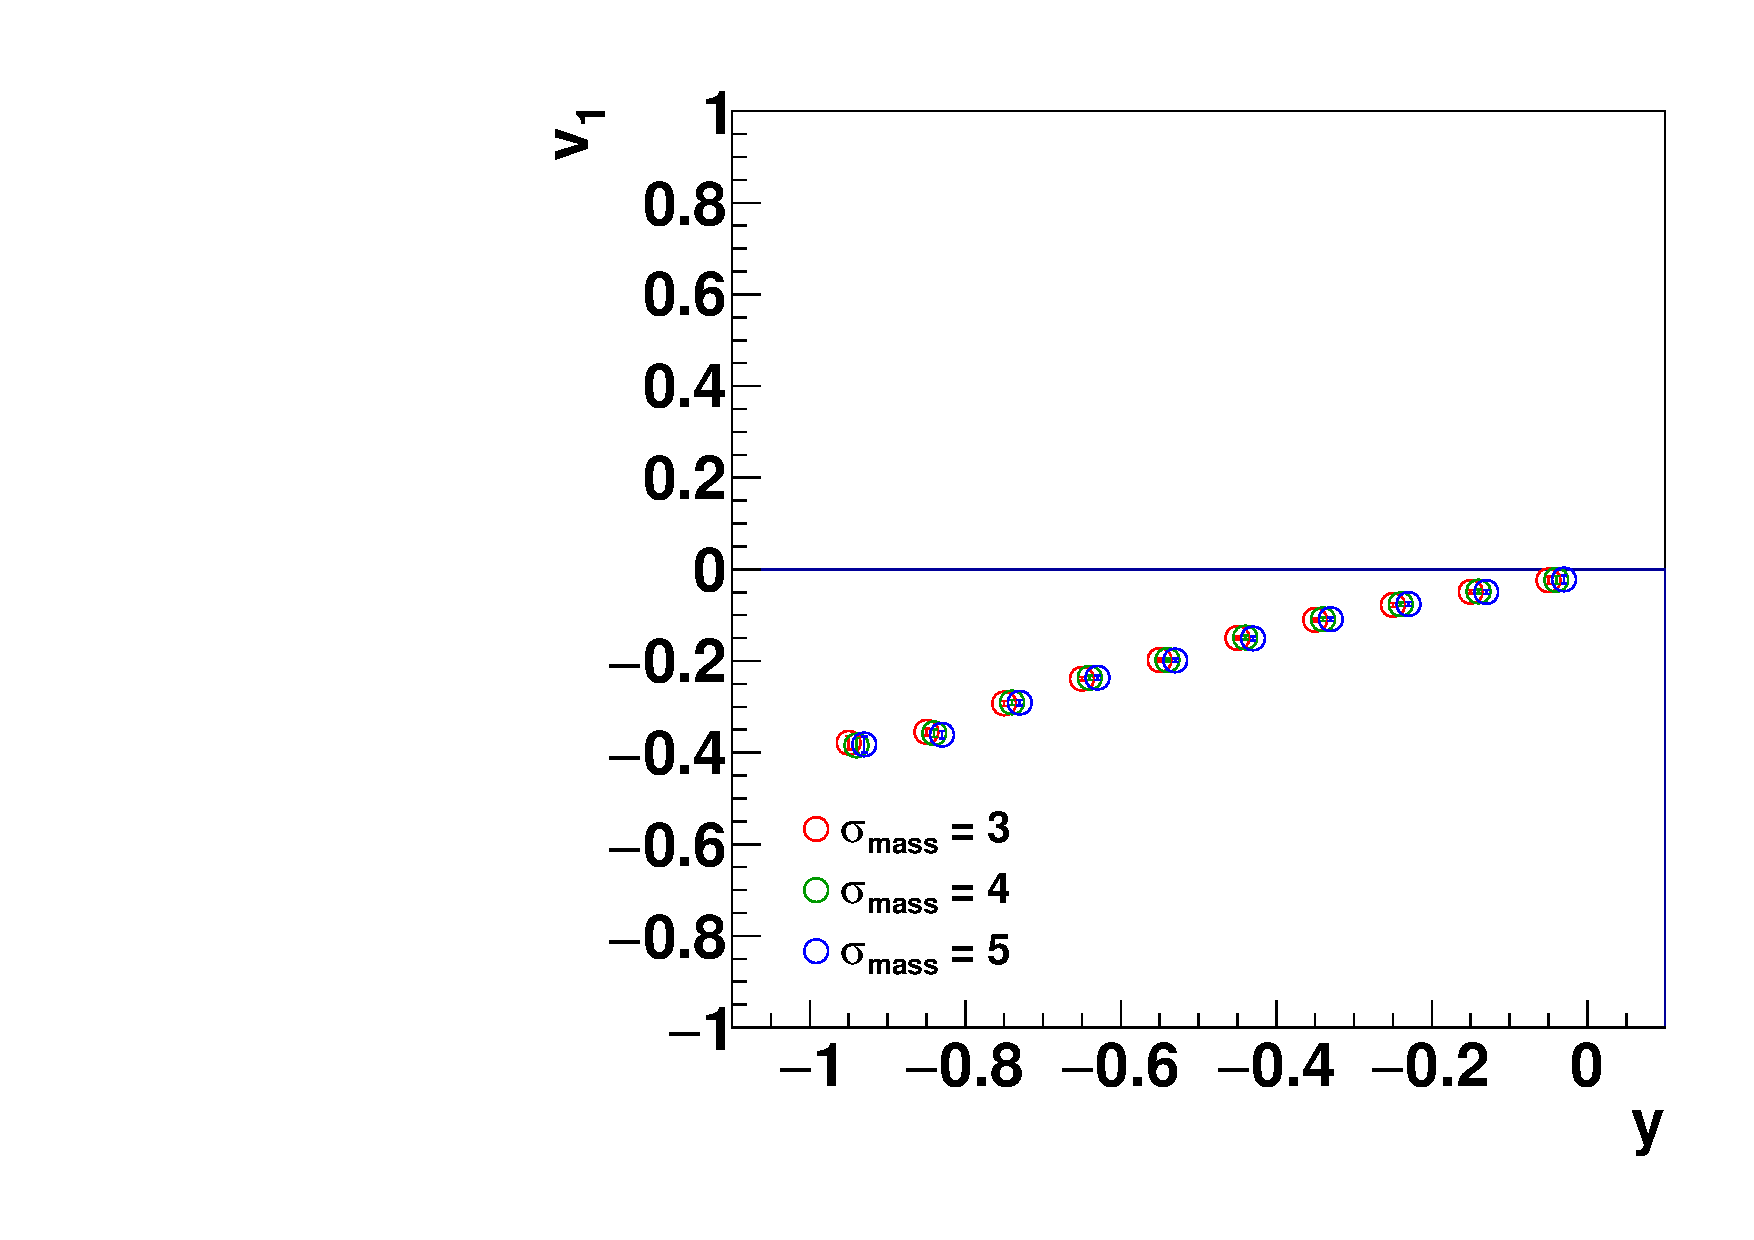
\includegraphics[width=0.49\linewidth]{FXT3gev/chapterX/fig/ld_sys_cut_v1_msigma.pdf}
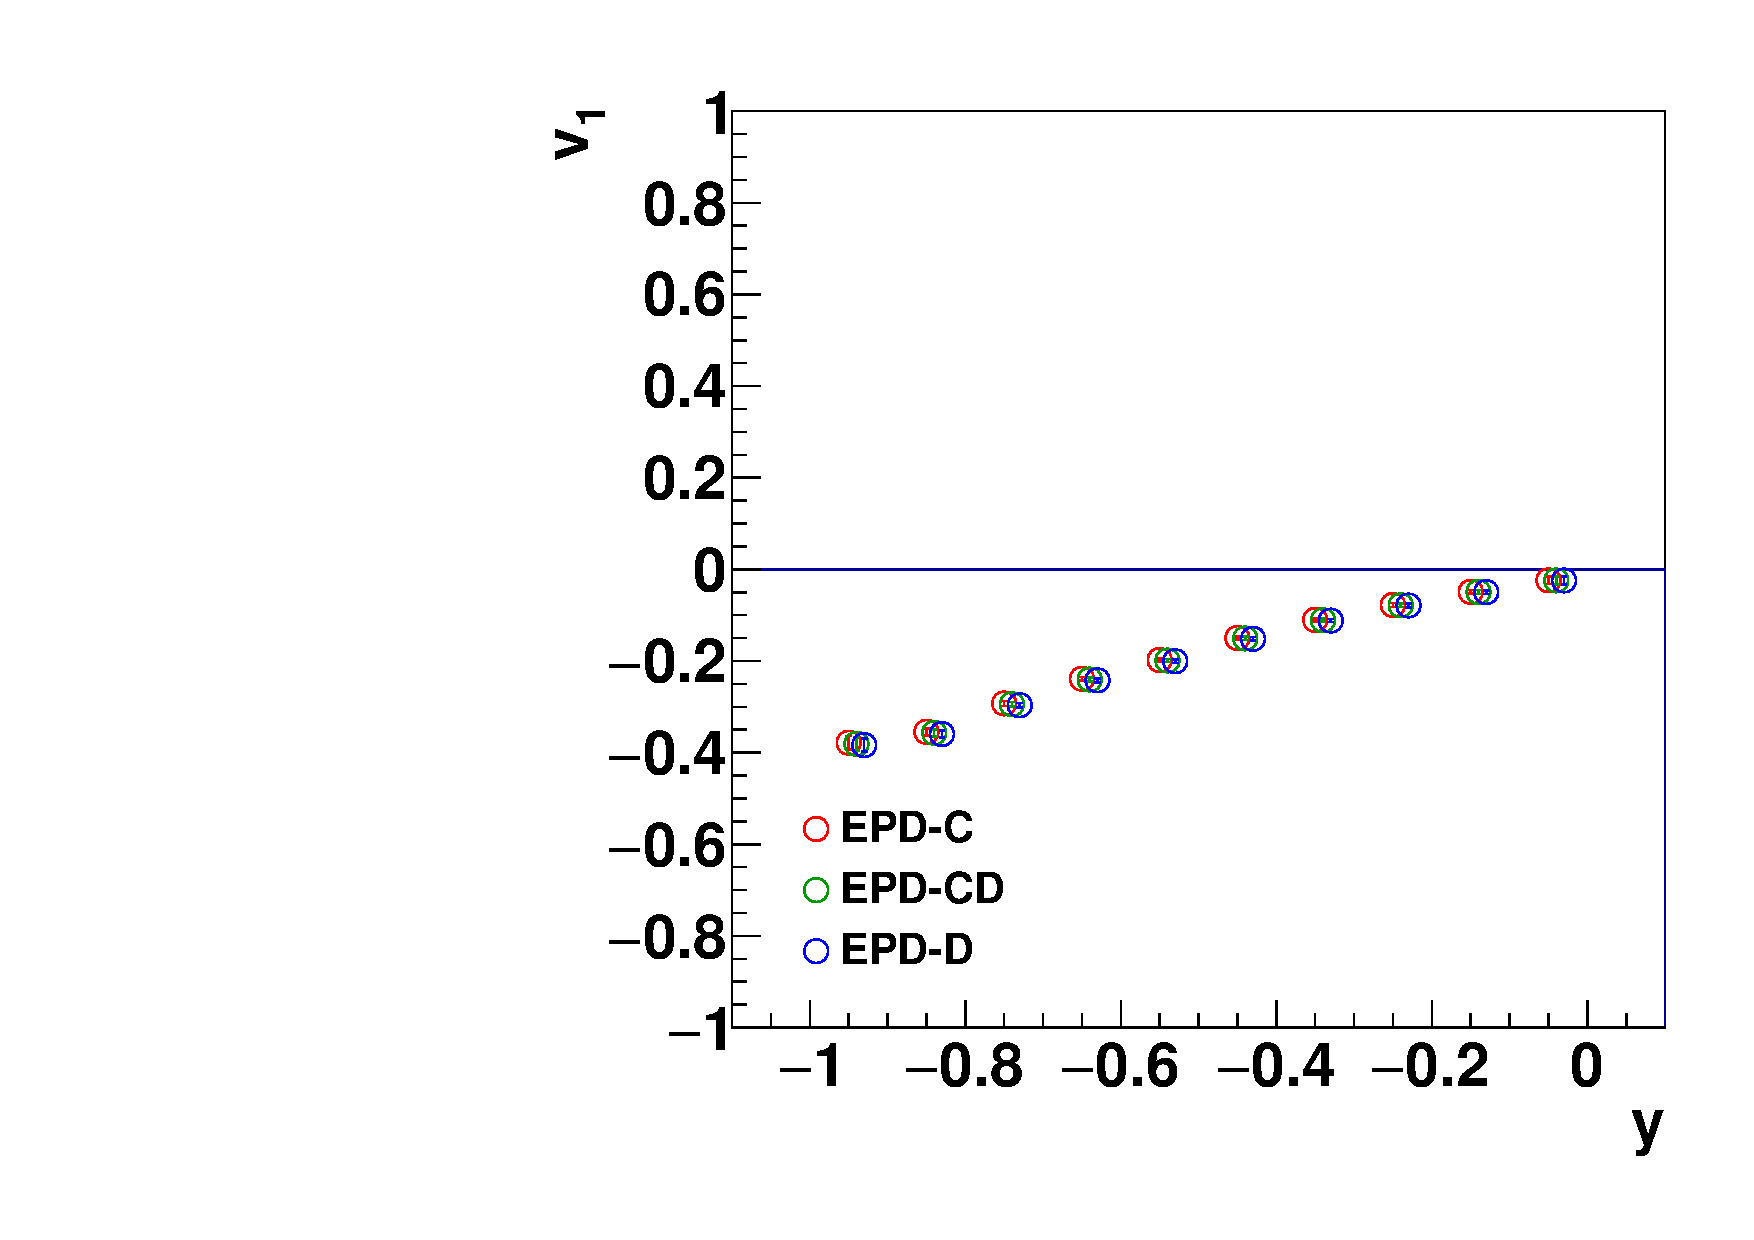
\includegraphics[width=0.49\linewidth]{FXT3gev/chapterX/fig/ld_sys_cut_v1_epdres.pdf}
\caption{Systematic uncertainty study for $v_{1}$ as a function of rapidity in 10-40\% for $\Lambda$ at $\sqrt{s_{NN}}$ = 3 GeV.}
\label{lambda_v1y_sys}
\end{figure}

\begin{figure}[h]
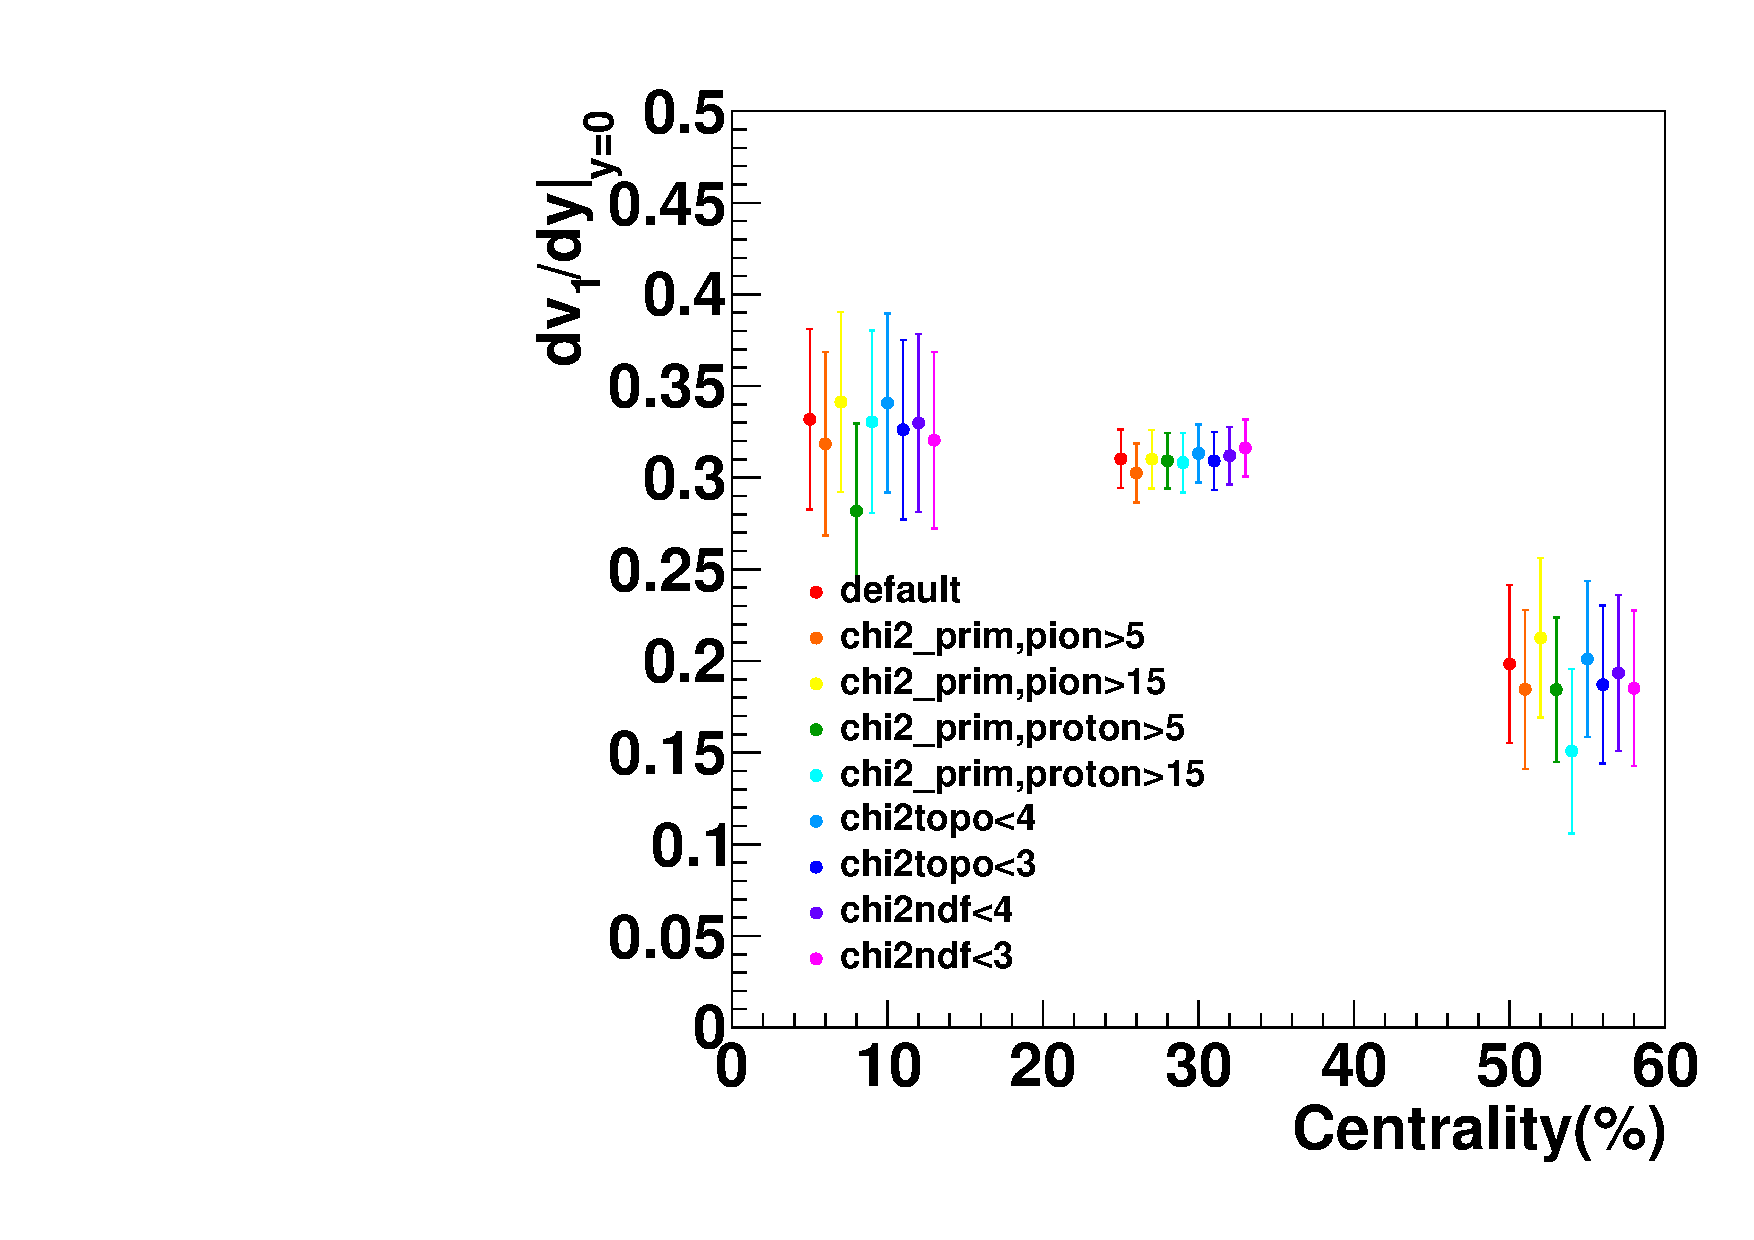
\includegraphics[width=0.49\linewidth]{chapterX/fig/ld_sys_cut_vn.pdf}
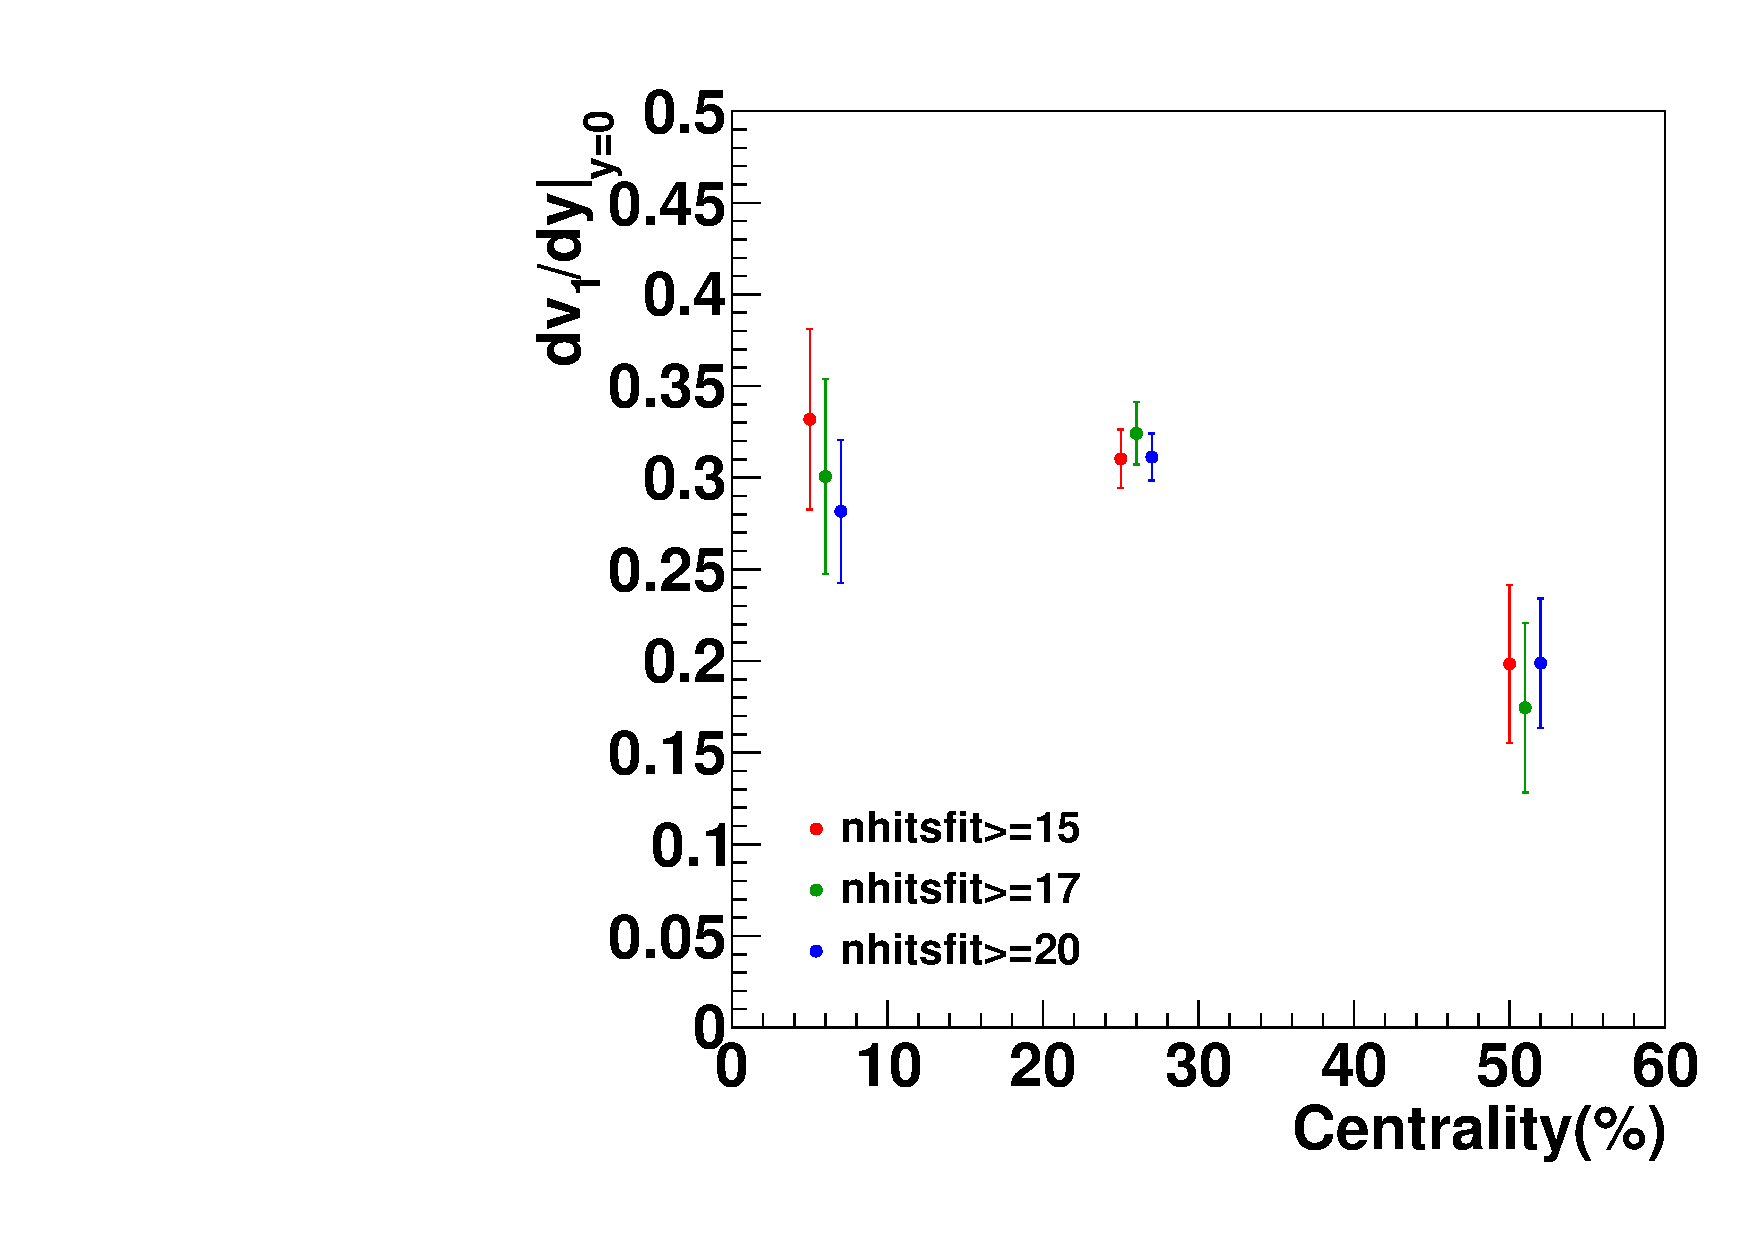
\includegraphics[width=0.49\linewidth]{chapterX/fig/ld_sys_cut_vn_nhits.pdf}
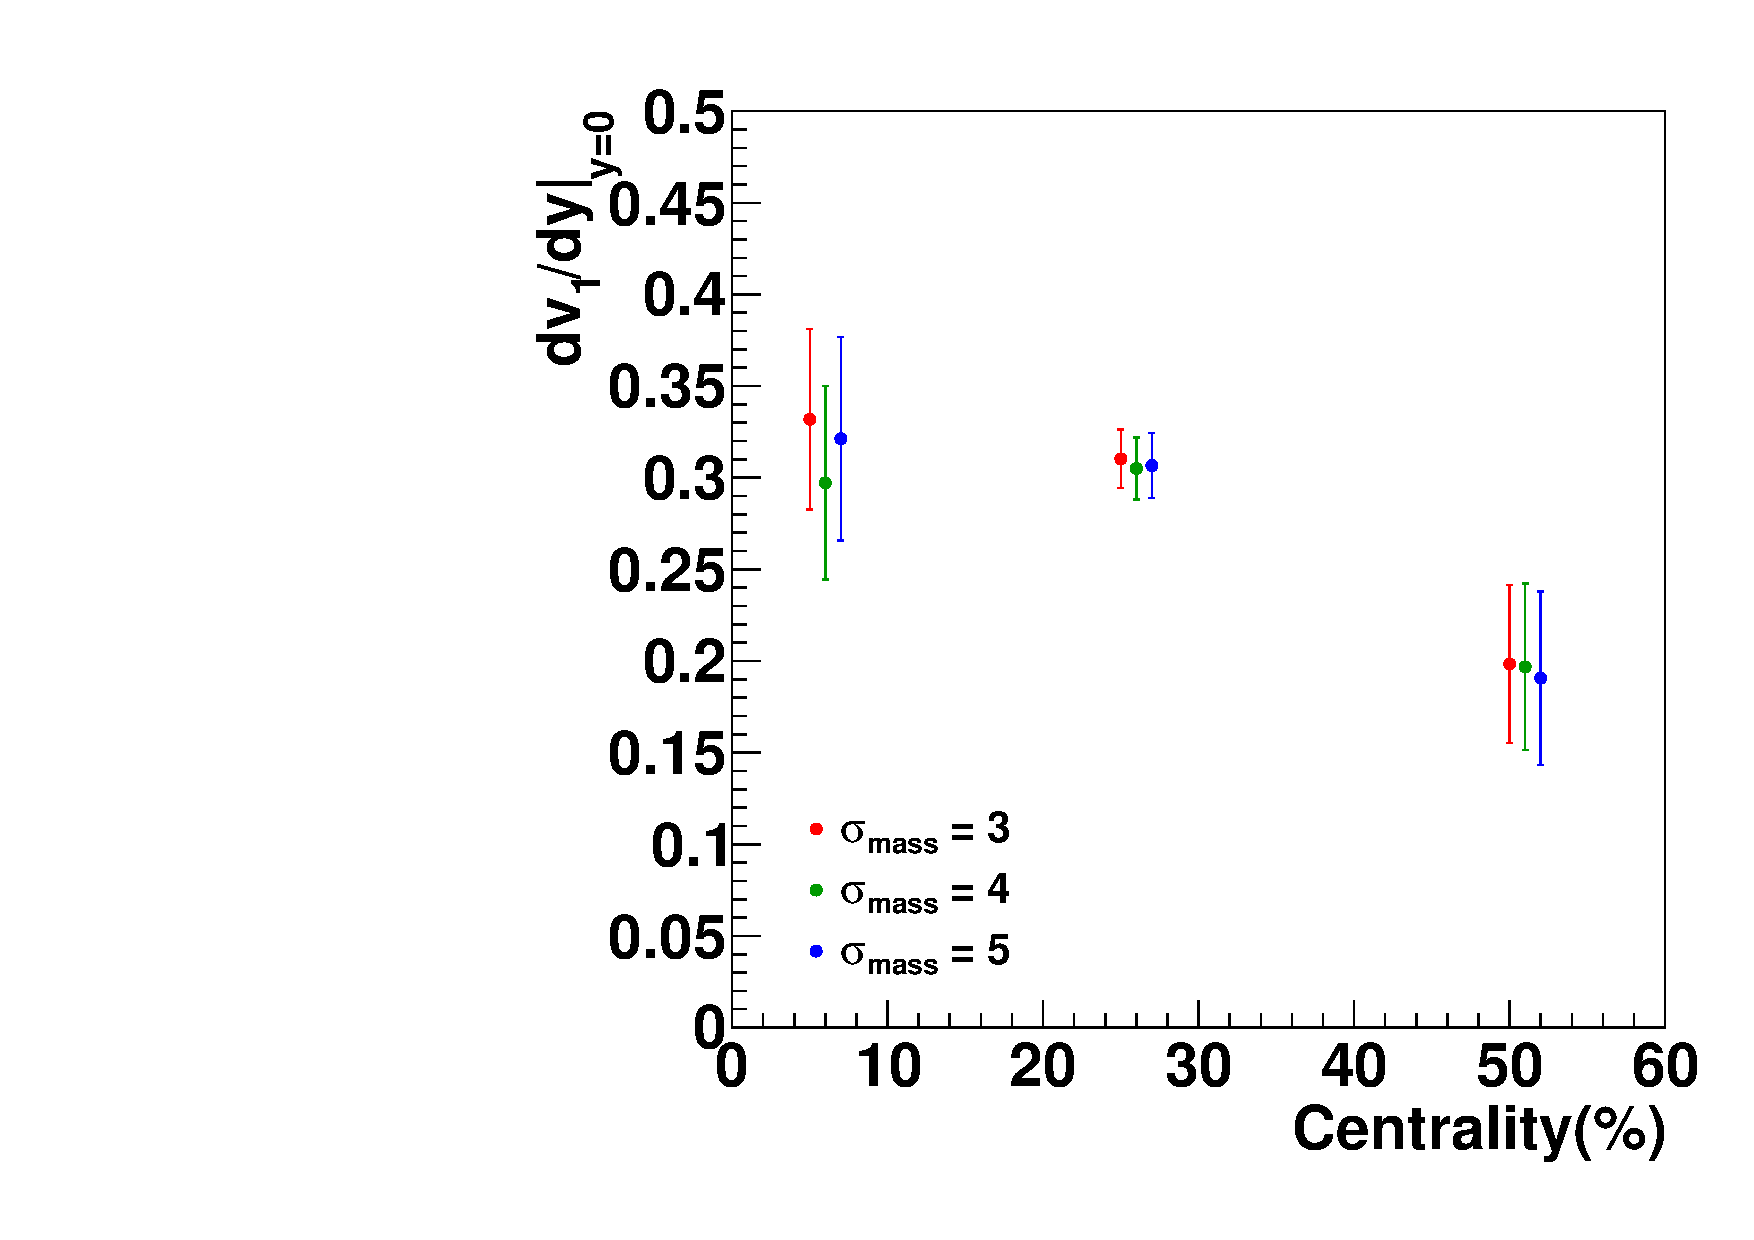
\includegraphics[width=0.49\linewidth]{FXT3gev/chapterX/fig/ld_sys_cut_vn_msigma.pdf}
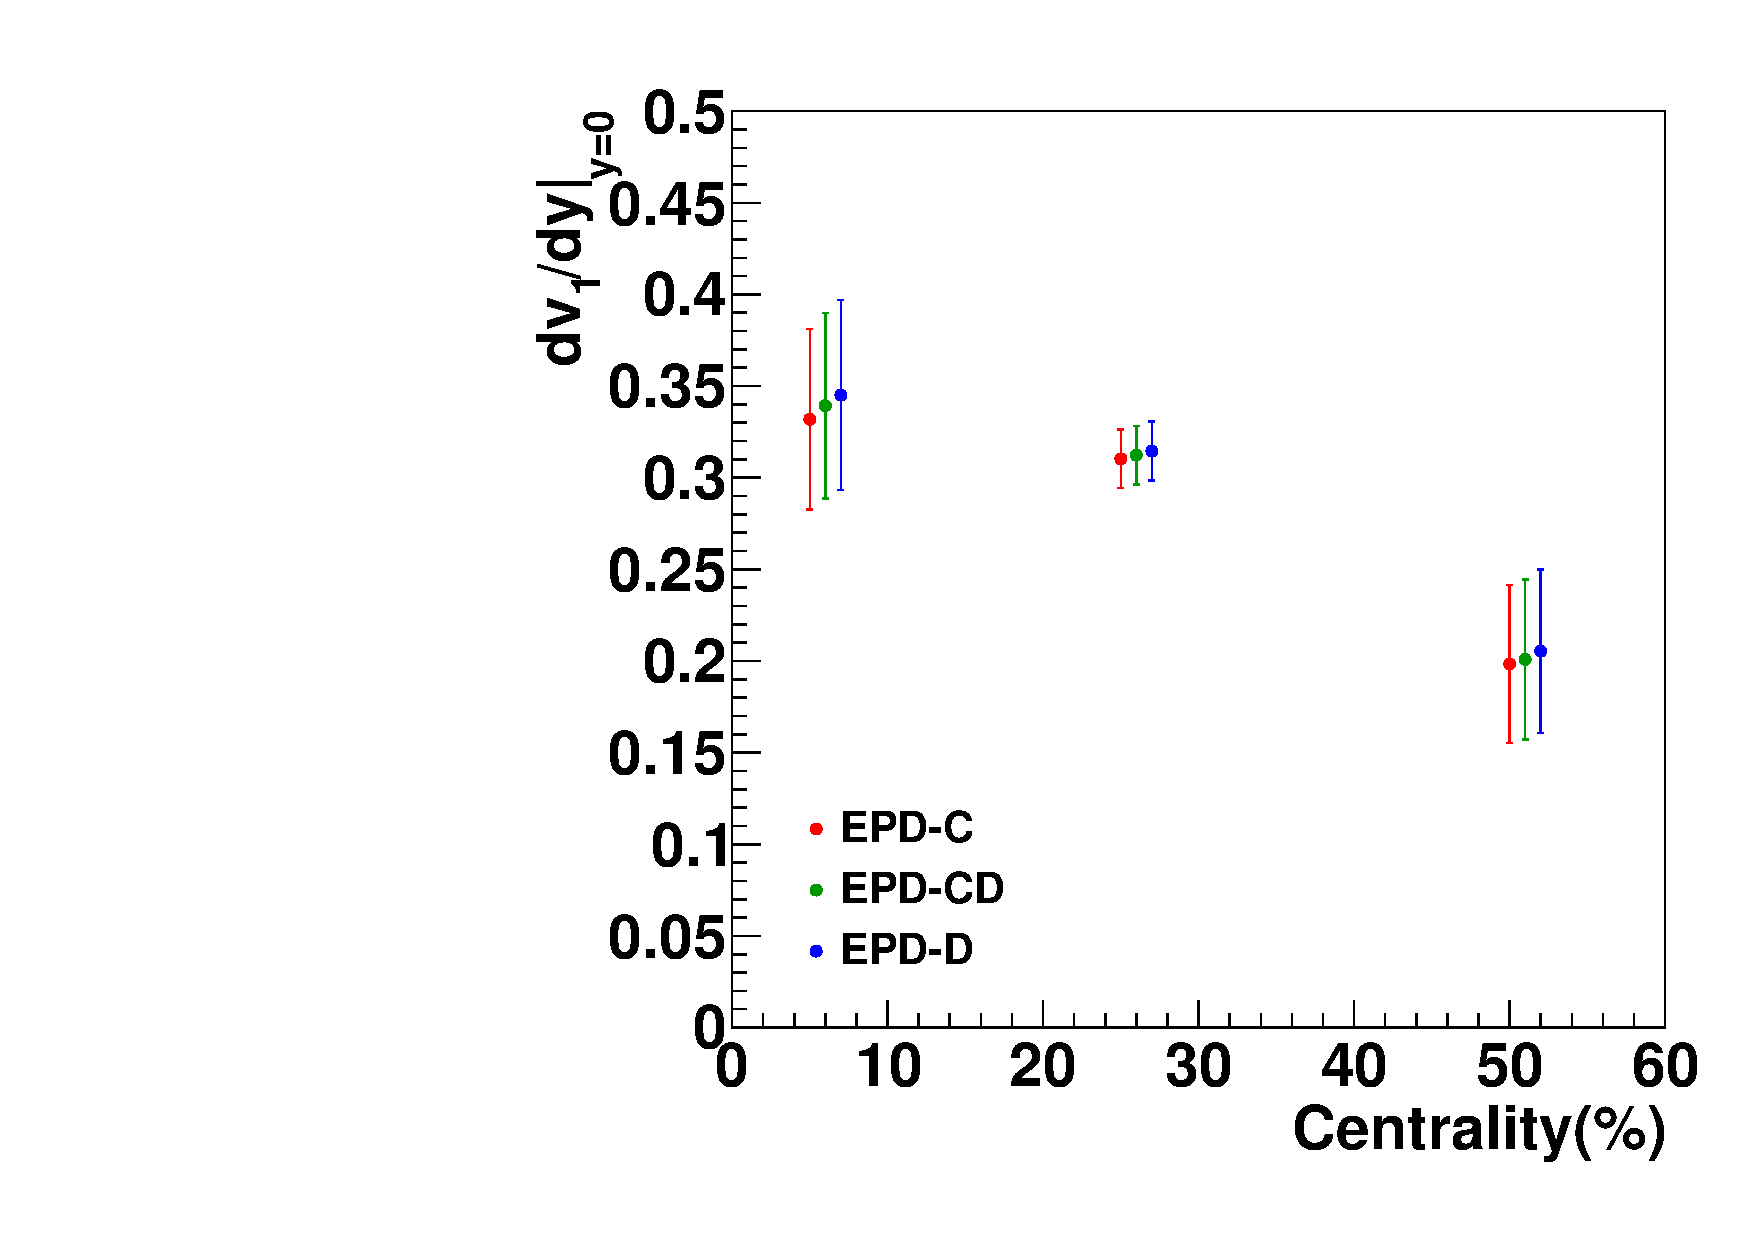
\includegraphics[width=0.49\linewidth]{FXT3gev/chapterX/fig/ld_sys_cut_vn_epdres.pdf}
\caption{Systematic uncertainty study for $dv_{1}/dy$ as a function of centrality for $\Lambda$ at $\sqrt{s_{NN}}$ = 3 GeV.}
\label{lambda_dv1dy_sys}
\end{figure}



\subsubsection{$v_2$}

\begin{figure}[h]
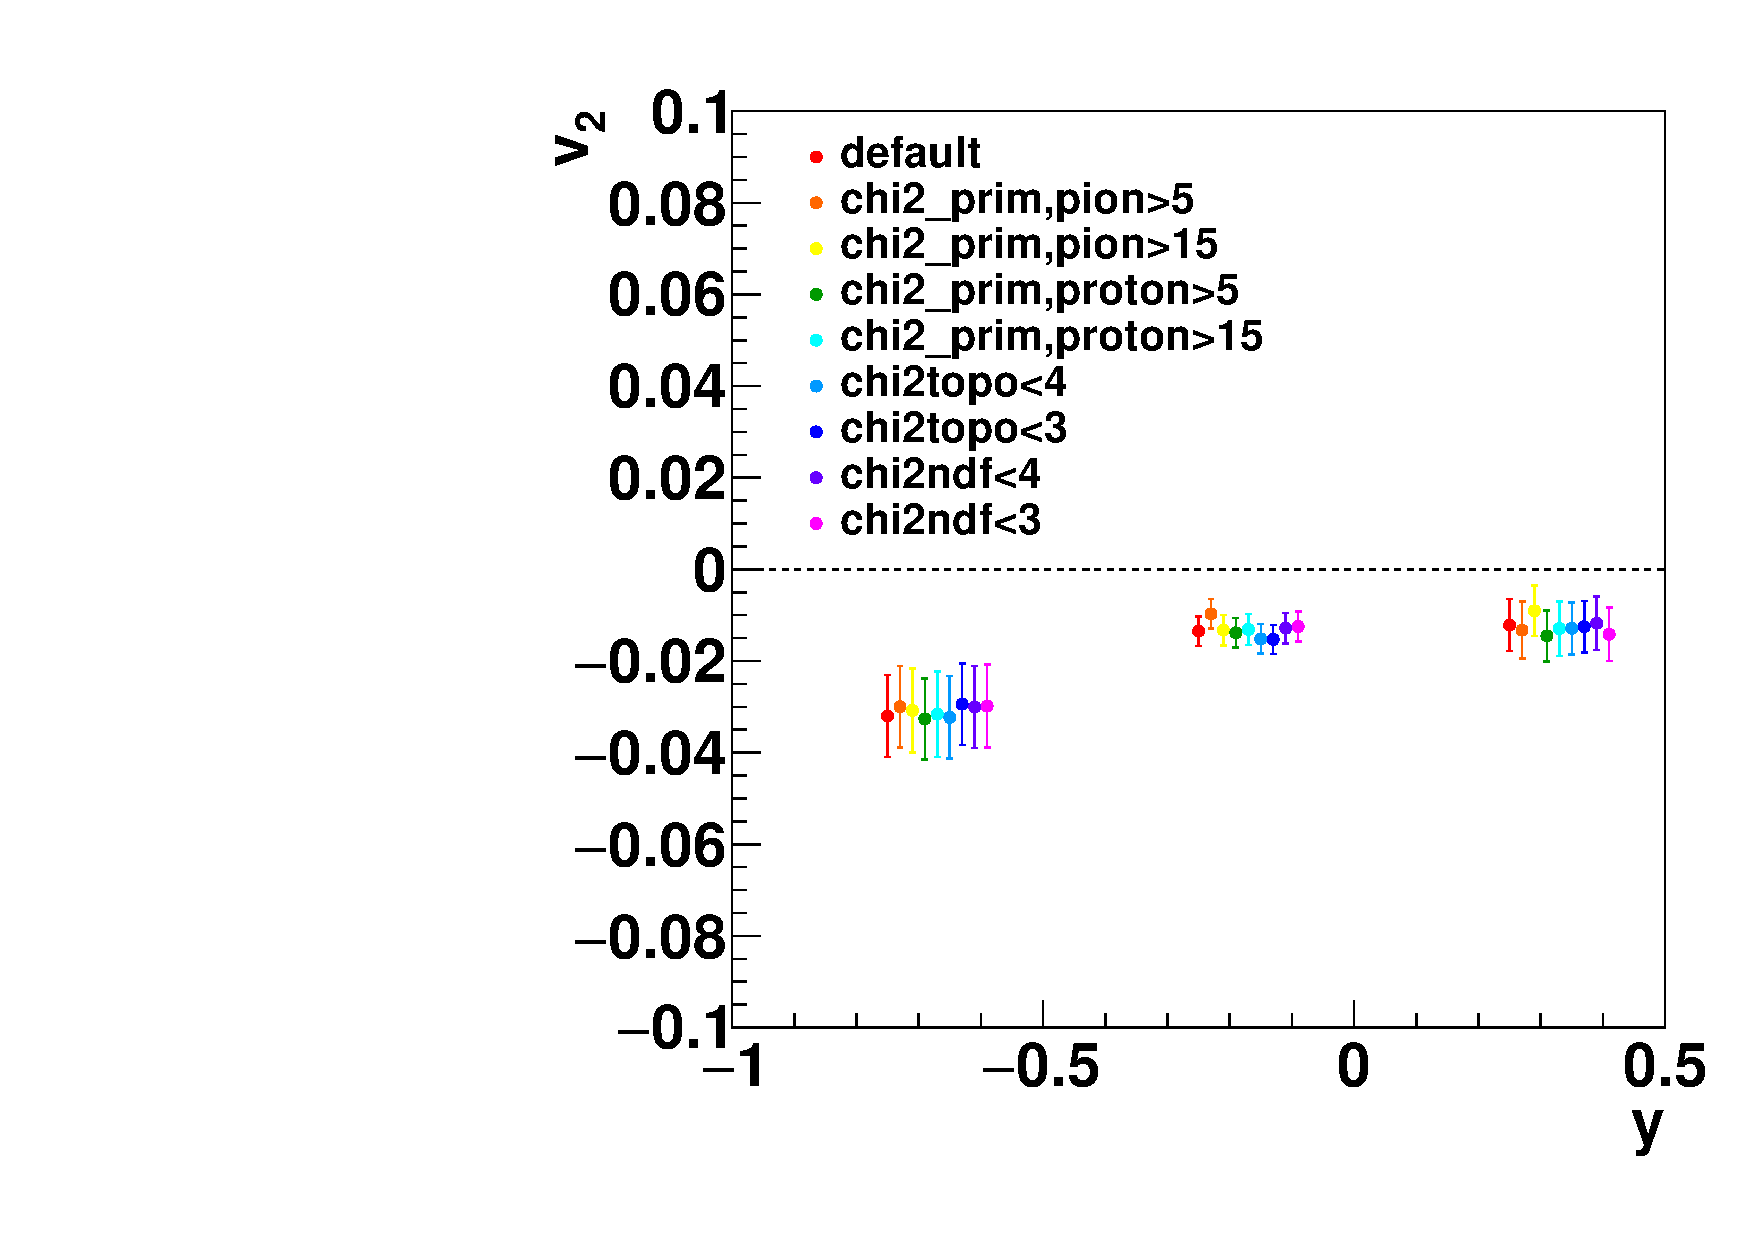
\includegraphics[width=0.49\linewidth]{chapterX/fig/ks_sys_cut_v2.pdf}
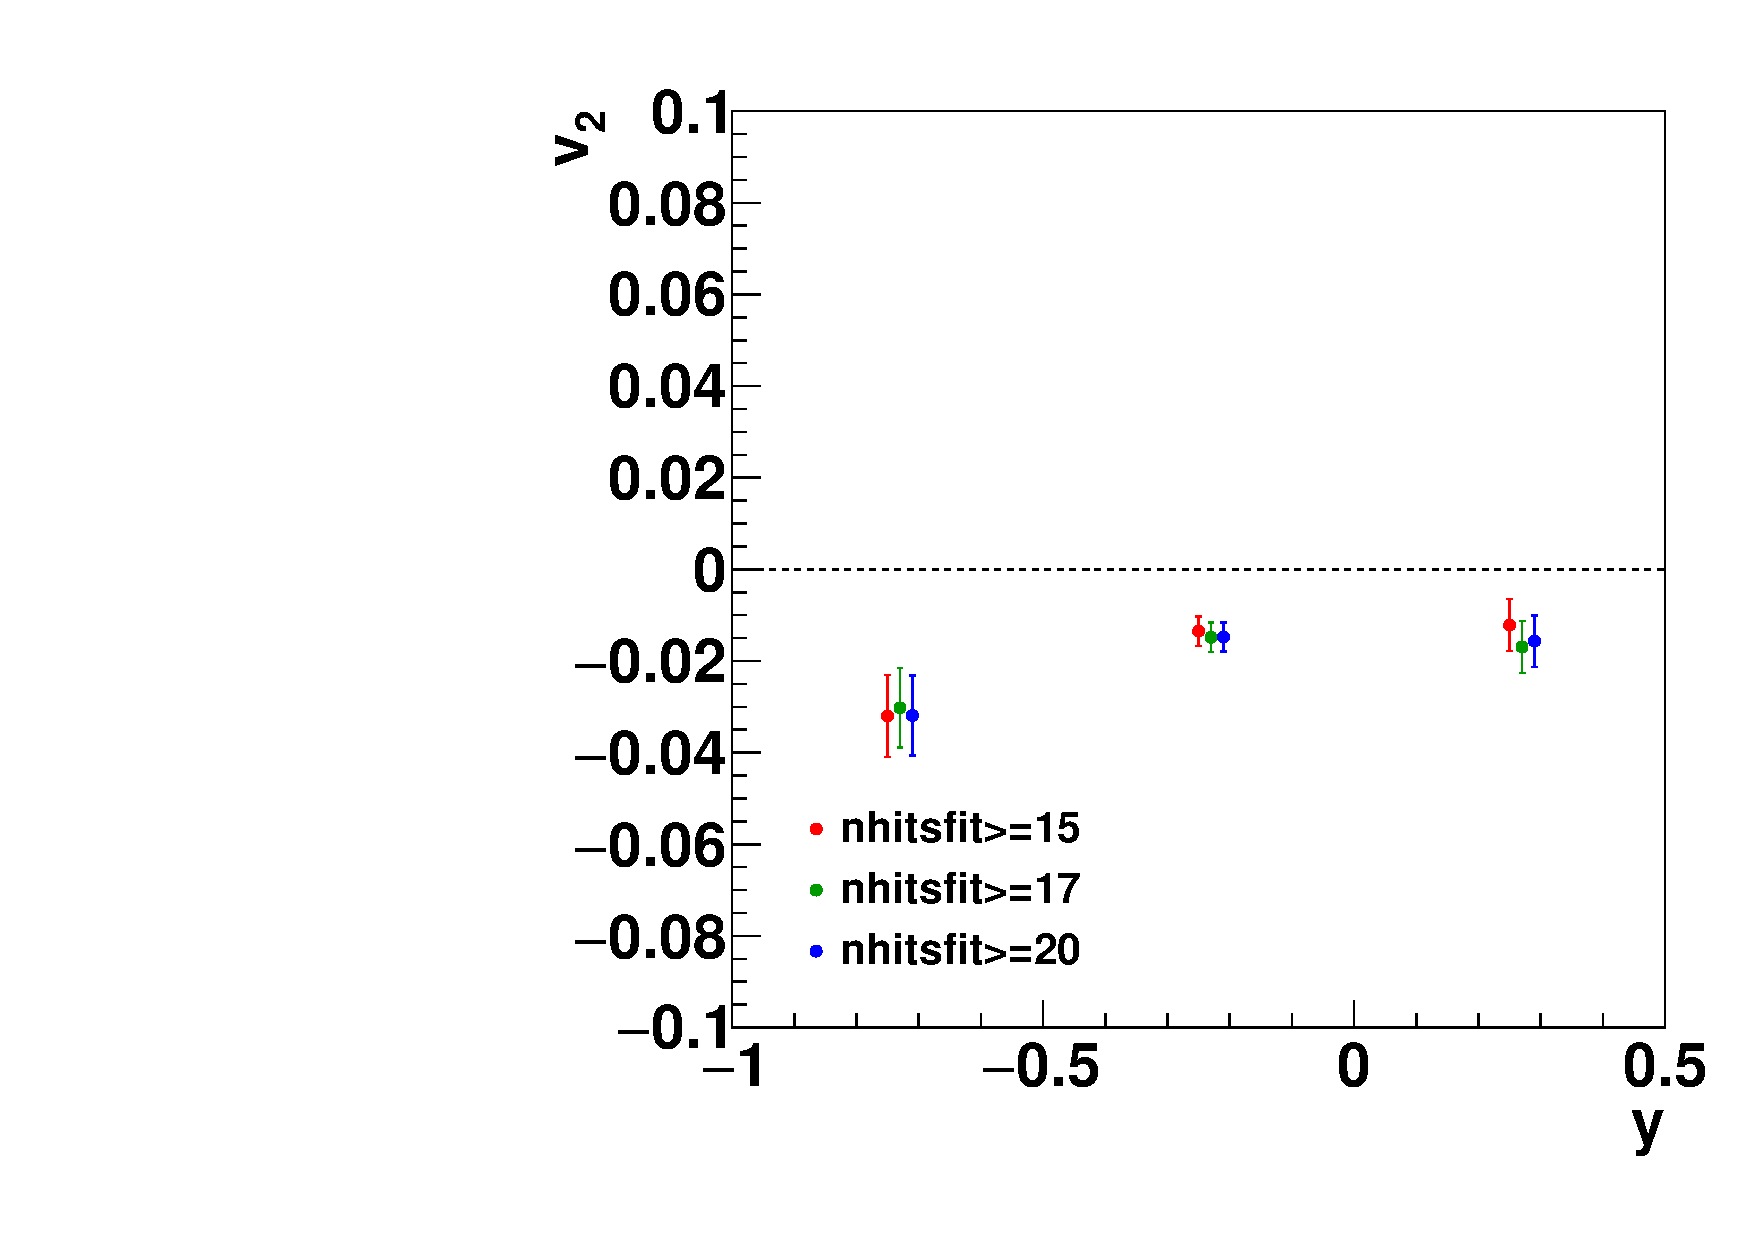
\includegraphics[width=0.49\linewidth]{chapterX/fig/ks_sys_cut_v2_nhits.pdf}
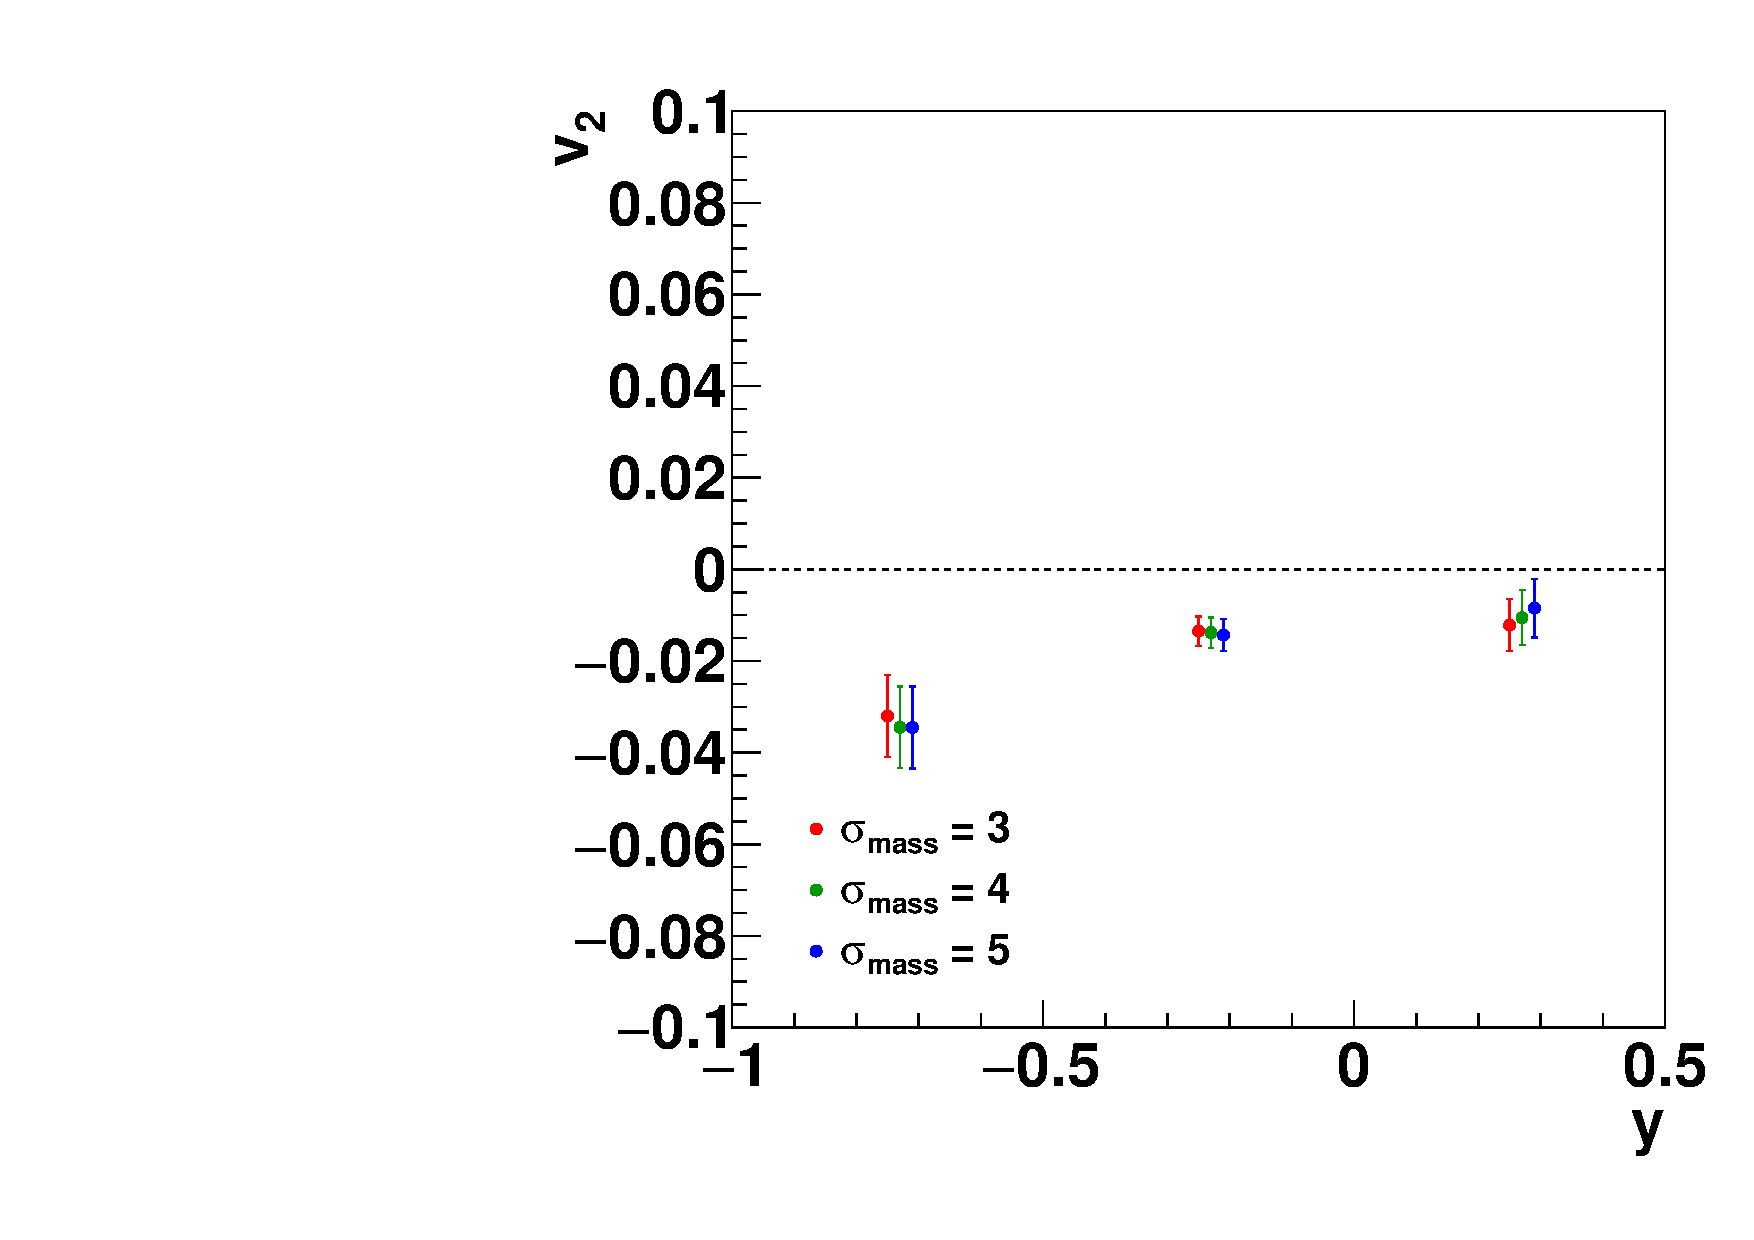
\includegraphics[width=0.49\linewidth]{FXT3gev/chapterX/fig/ks_sys_cut_v2_msigma.pdf}
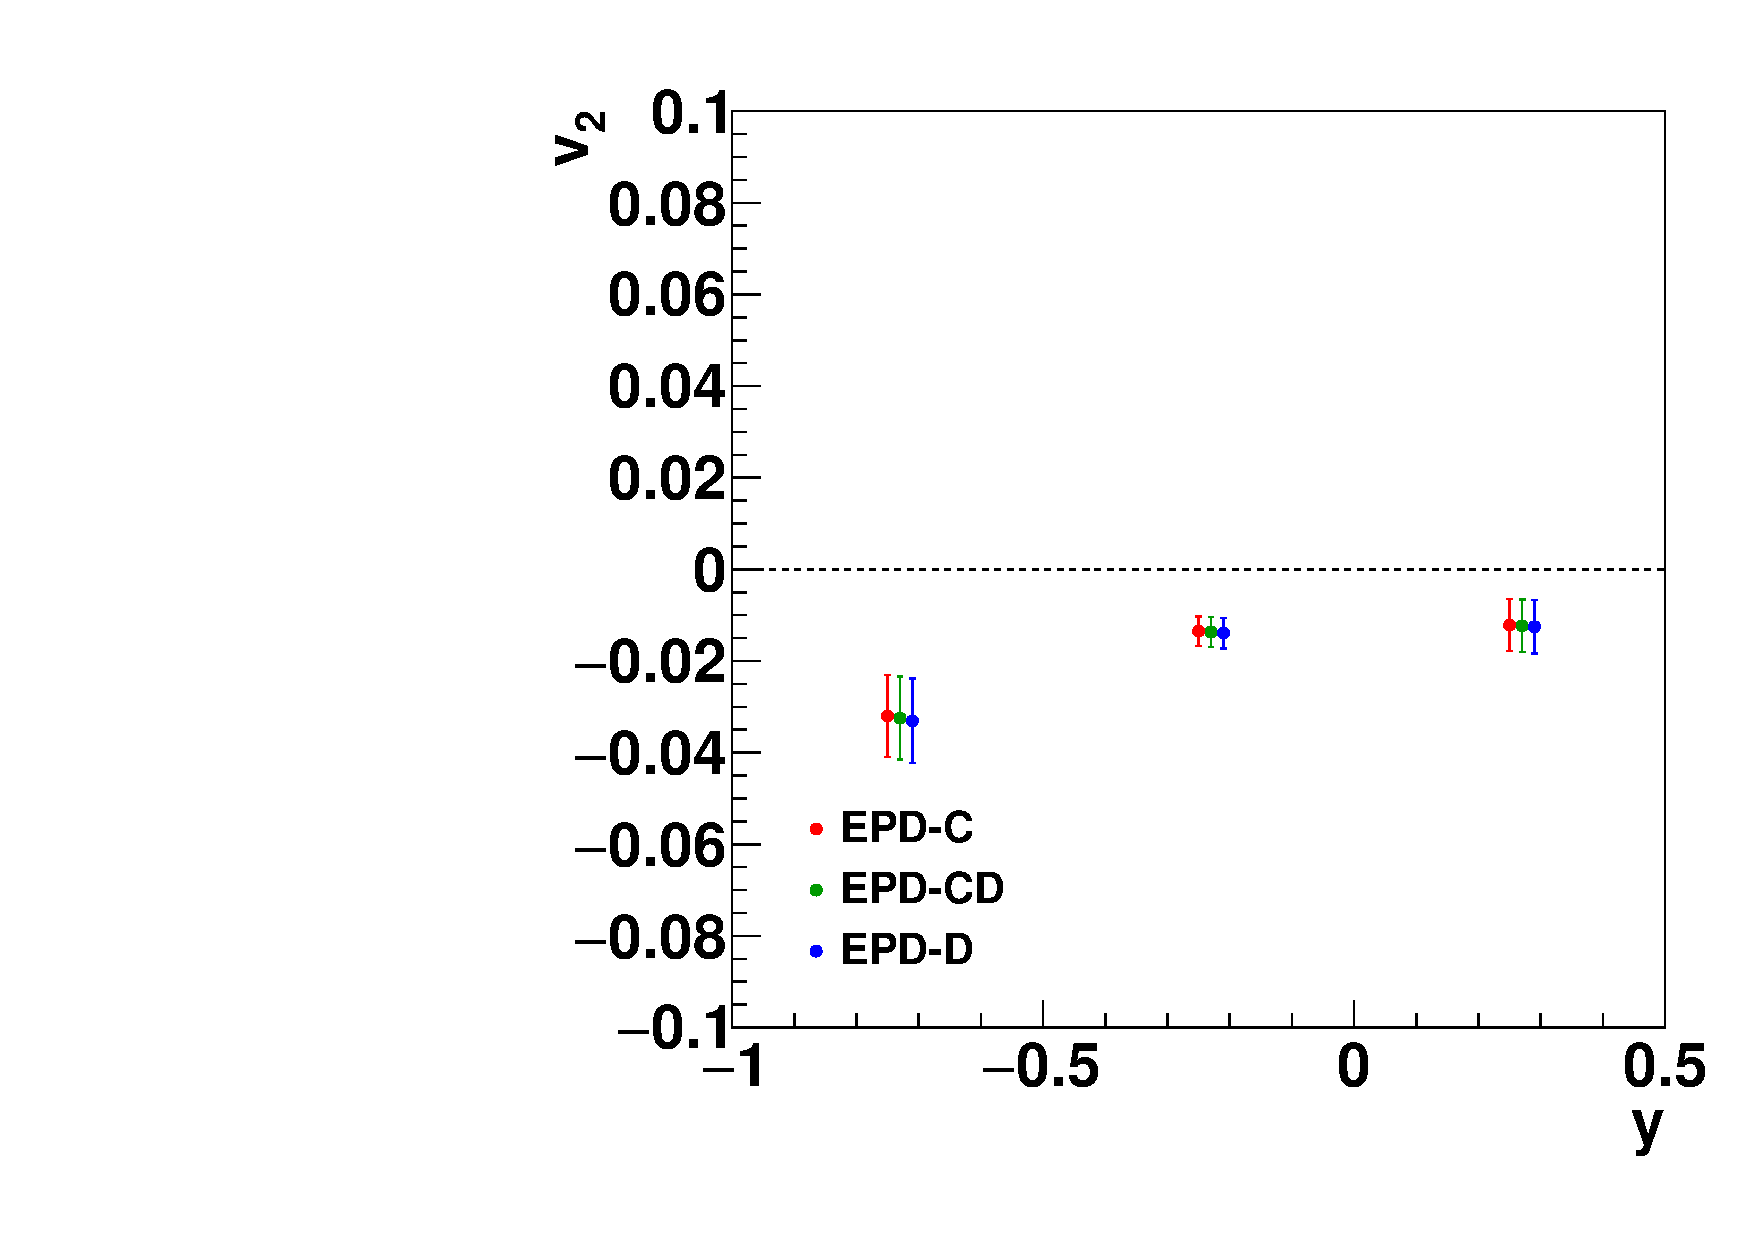
\includegraphics[width=0.49\linewidth]{FXT3gev/chapterX/fig/ks_sys_cut_v2_epdres.pdf}
\caption{Systematic uncertainty study for $v_{2}$ as a function of rapidity in 10-40\% for $K^0_S$ at $\sqrt{s_{NN}}$ = 3 GeV.}
\label{ks_v1y_sys}
\end{figure}




\begin{figure}[h]
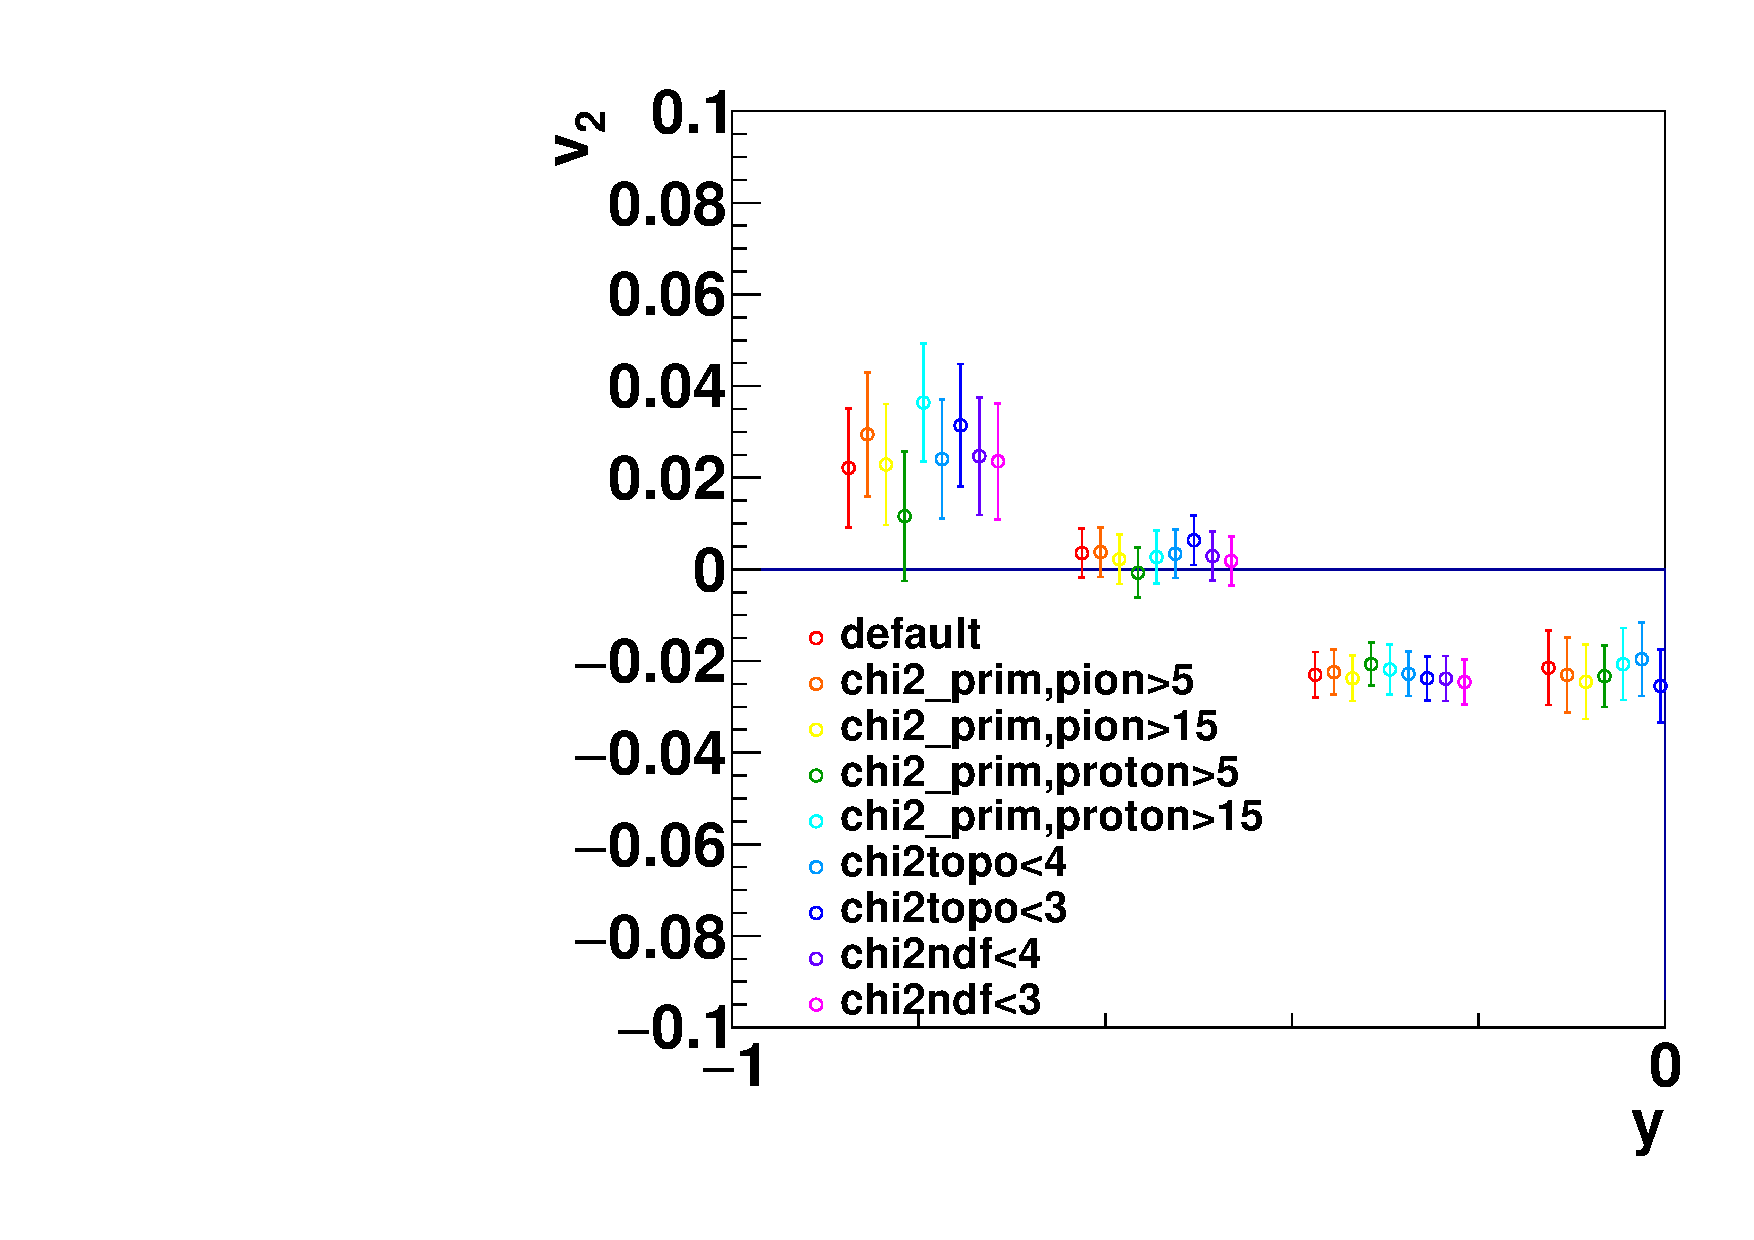
\includegraphics[width=0.49\linewidth]{chapterX/fig/ld_sys_cut_v2.pdf}
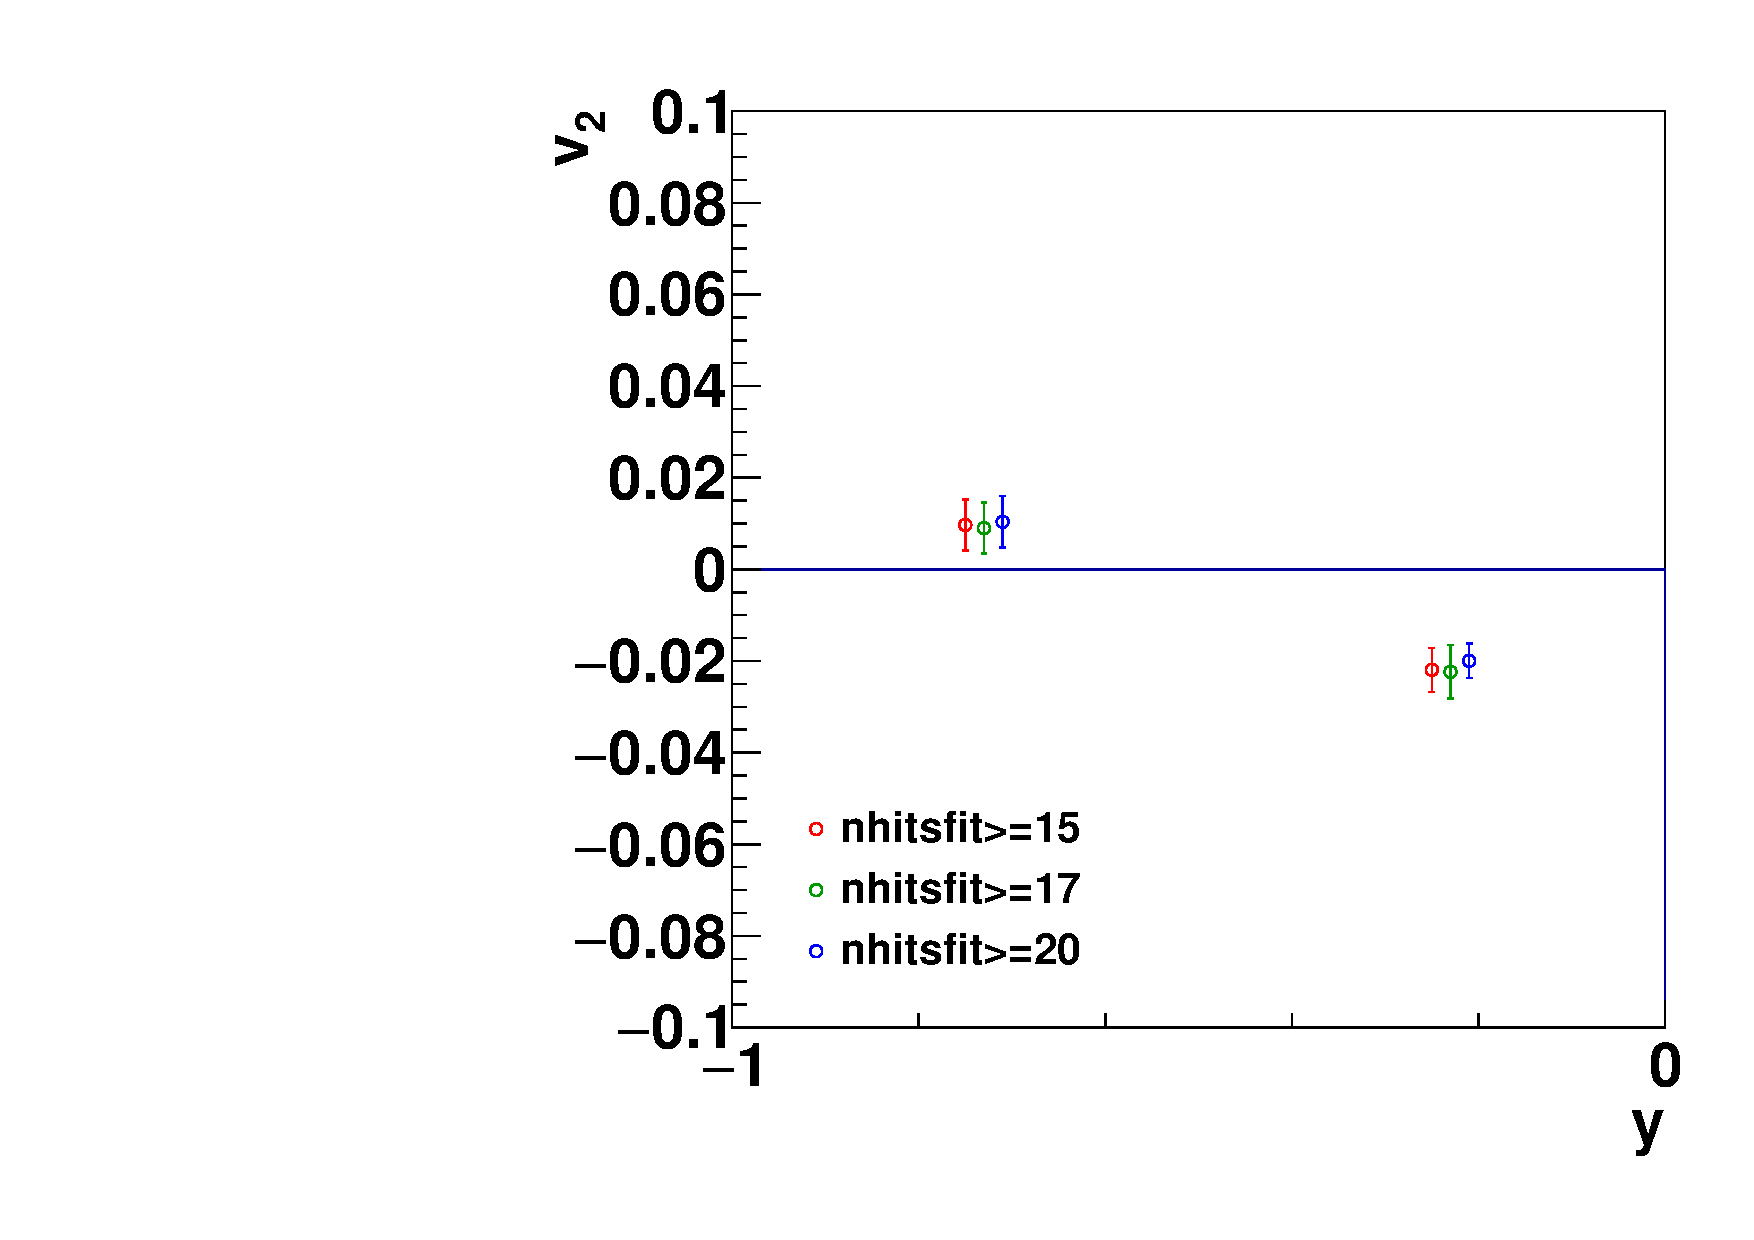
\includegraphics[width=0.49\linewidth]{chapterX/fig/ld_sys_cut_v2_nhits.pdf}
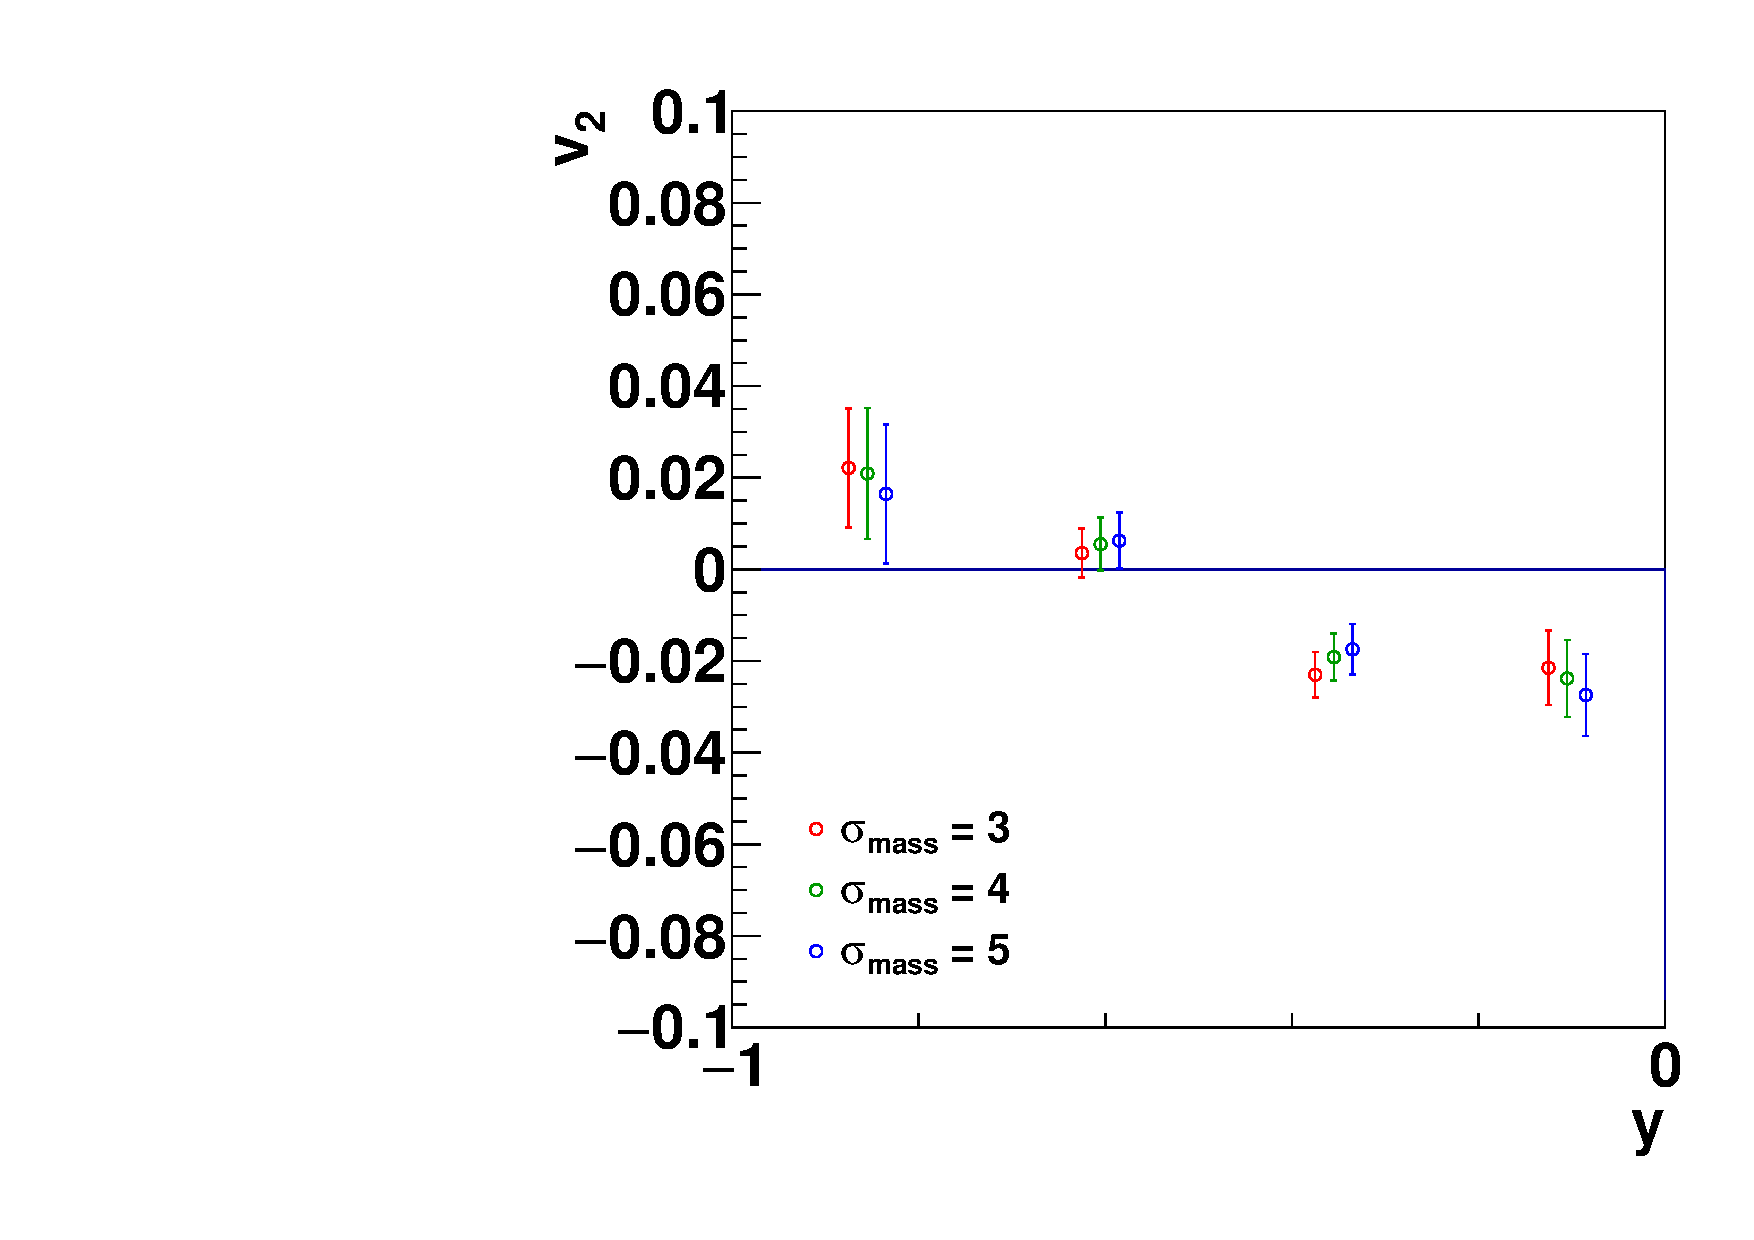
\includegraphics[width=0.49\linewidth]{FXT3gev/chapterX/fig/ld_sys_cut_v2_msigma.pdf}
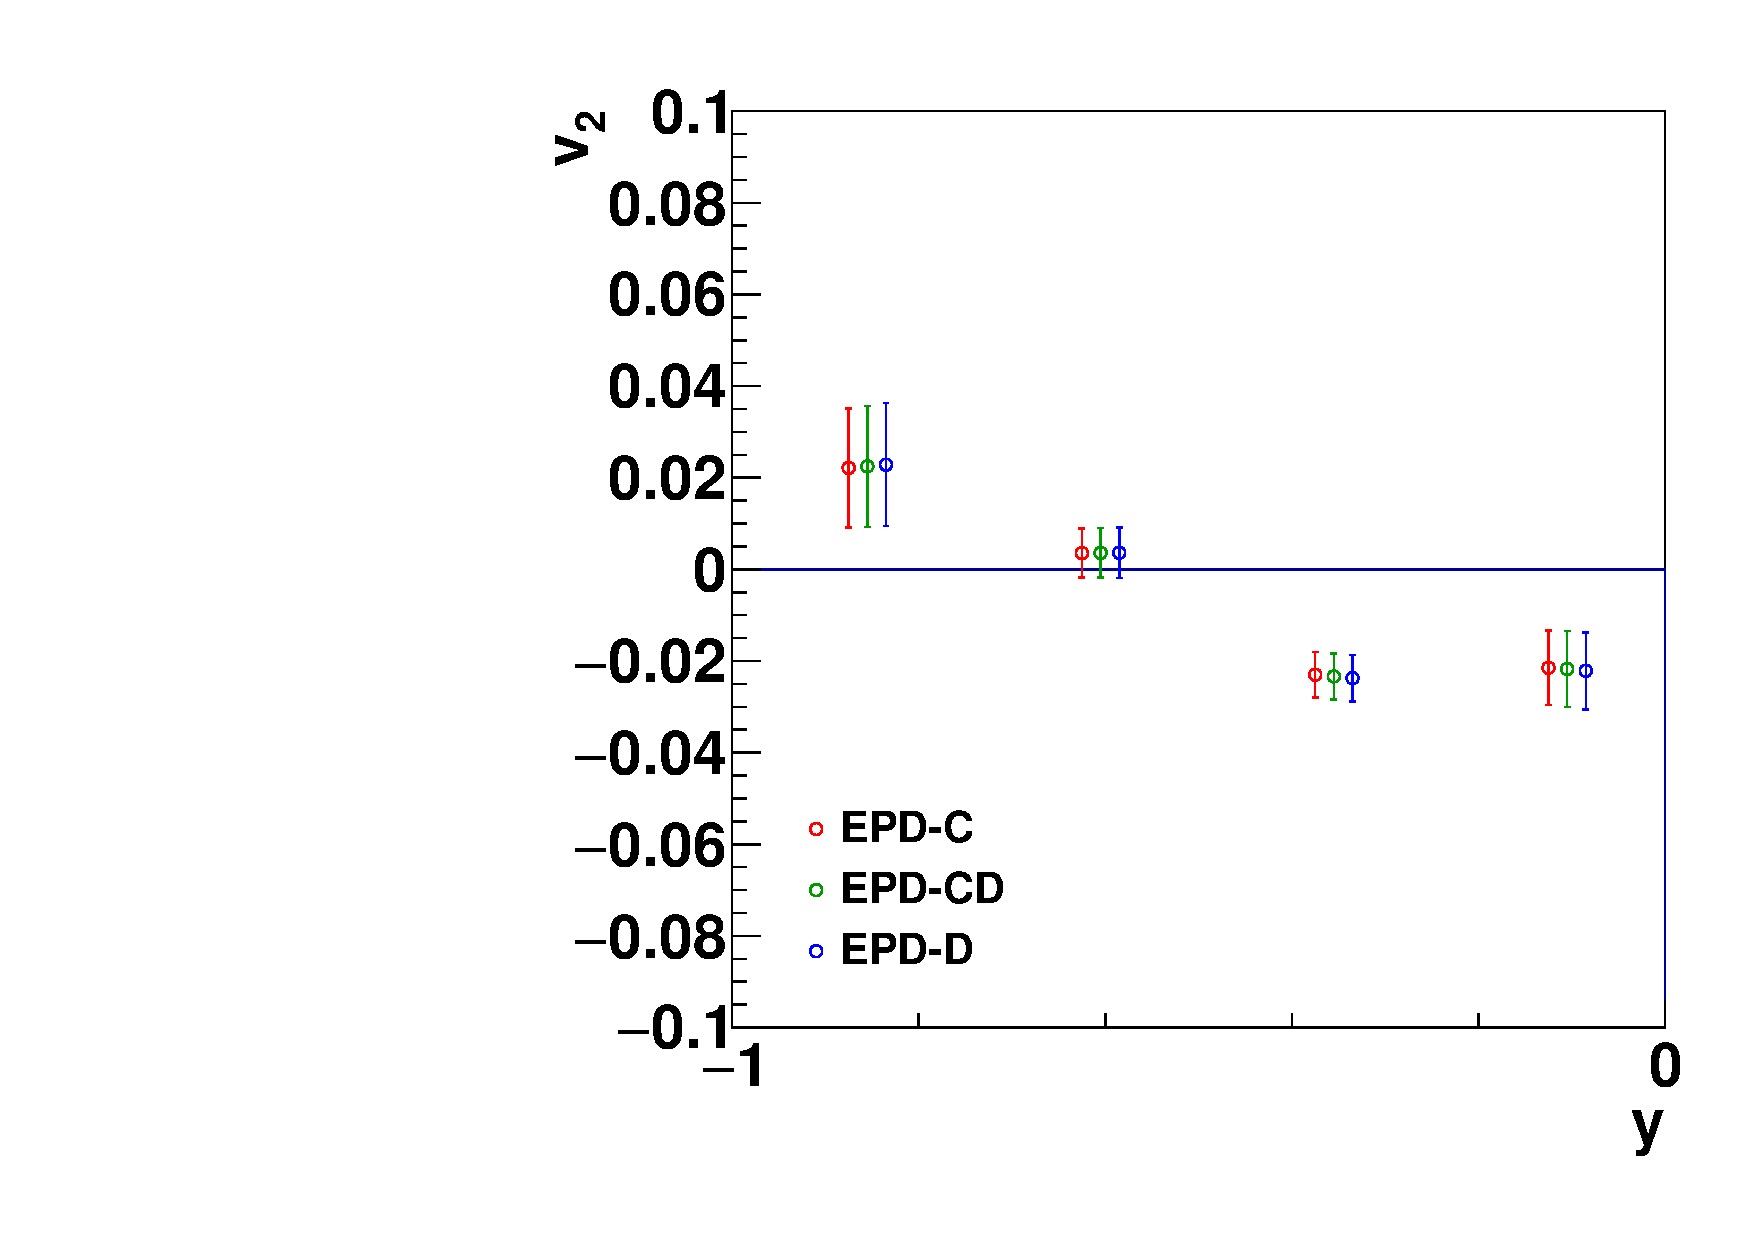
\includegraphics[width=0.49\linewidth]{FXT3gev/chapterX/fig/ld_sys_cut_v2_epdres.pdf}
\caption{Systematic uncertainty study for $v_{2}$ as a function of rapidity in 10-40\% for $\Lambda$ at $\sqrt{s_{NN}}$ = 3 GeV.}
\label{lambda_v2y_sys}
\end{figure}




\subsection{Results}
\subsubsection{$v_1$ results for $K^0_S$, $\Lambda$}

\begin{figure}[h]
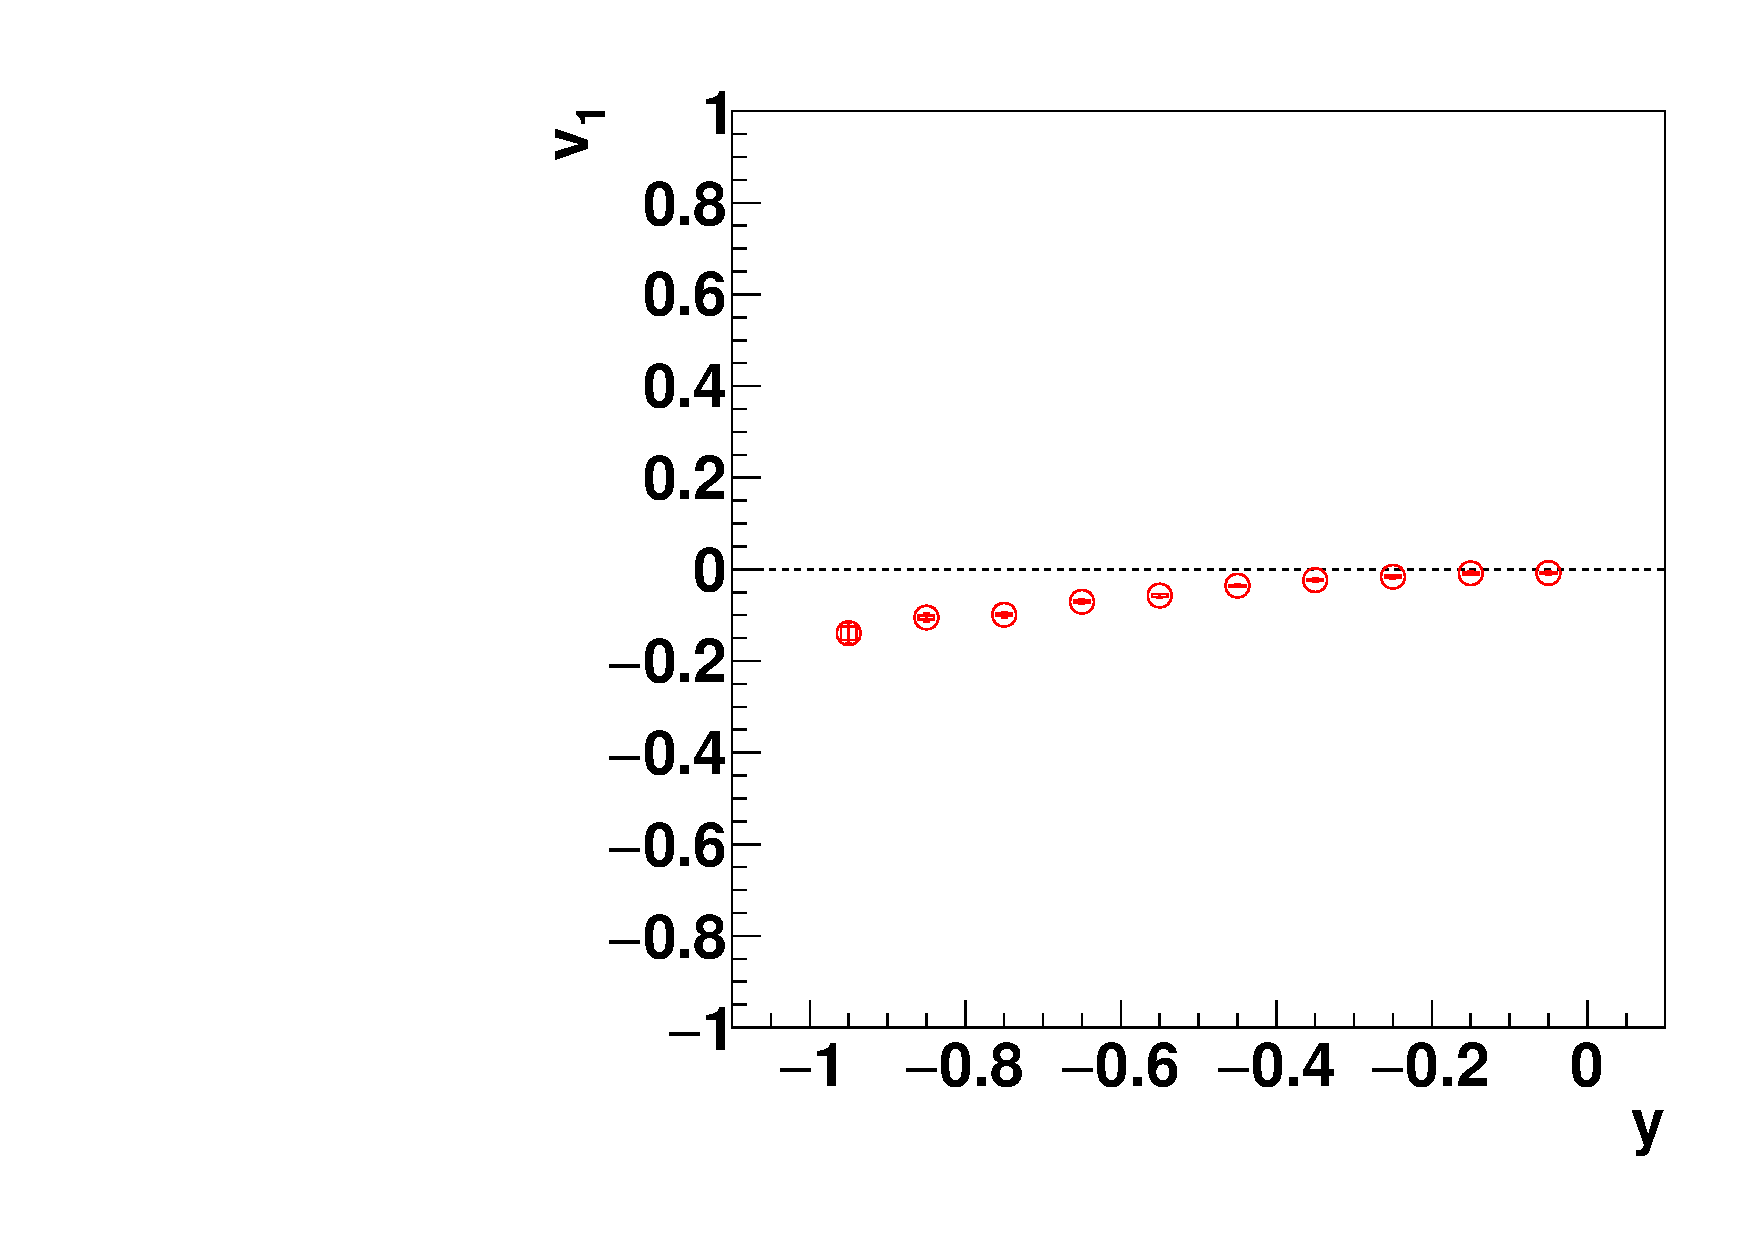
\includegraphics[width=0.49\linewidth]{chapterX/fig/ks_sys_v1.pdf}
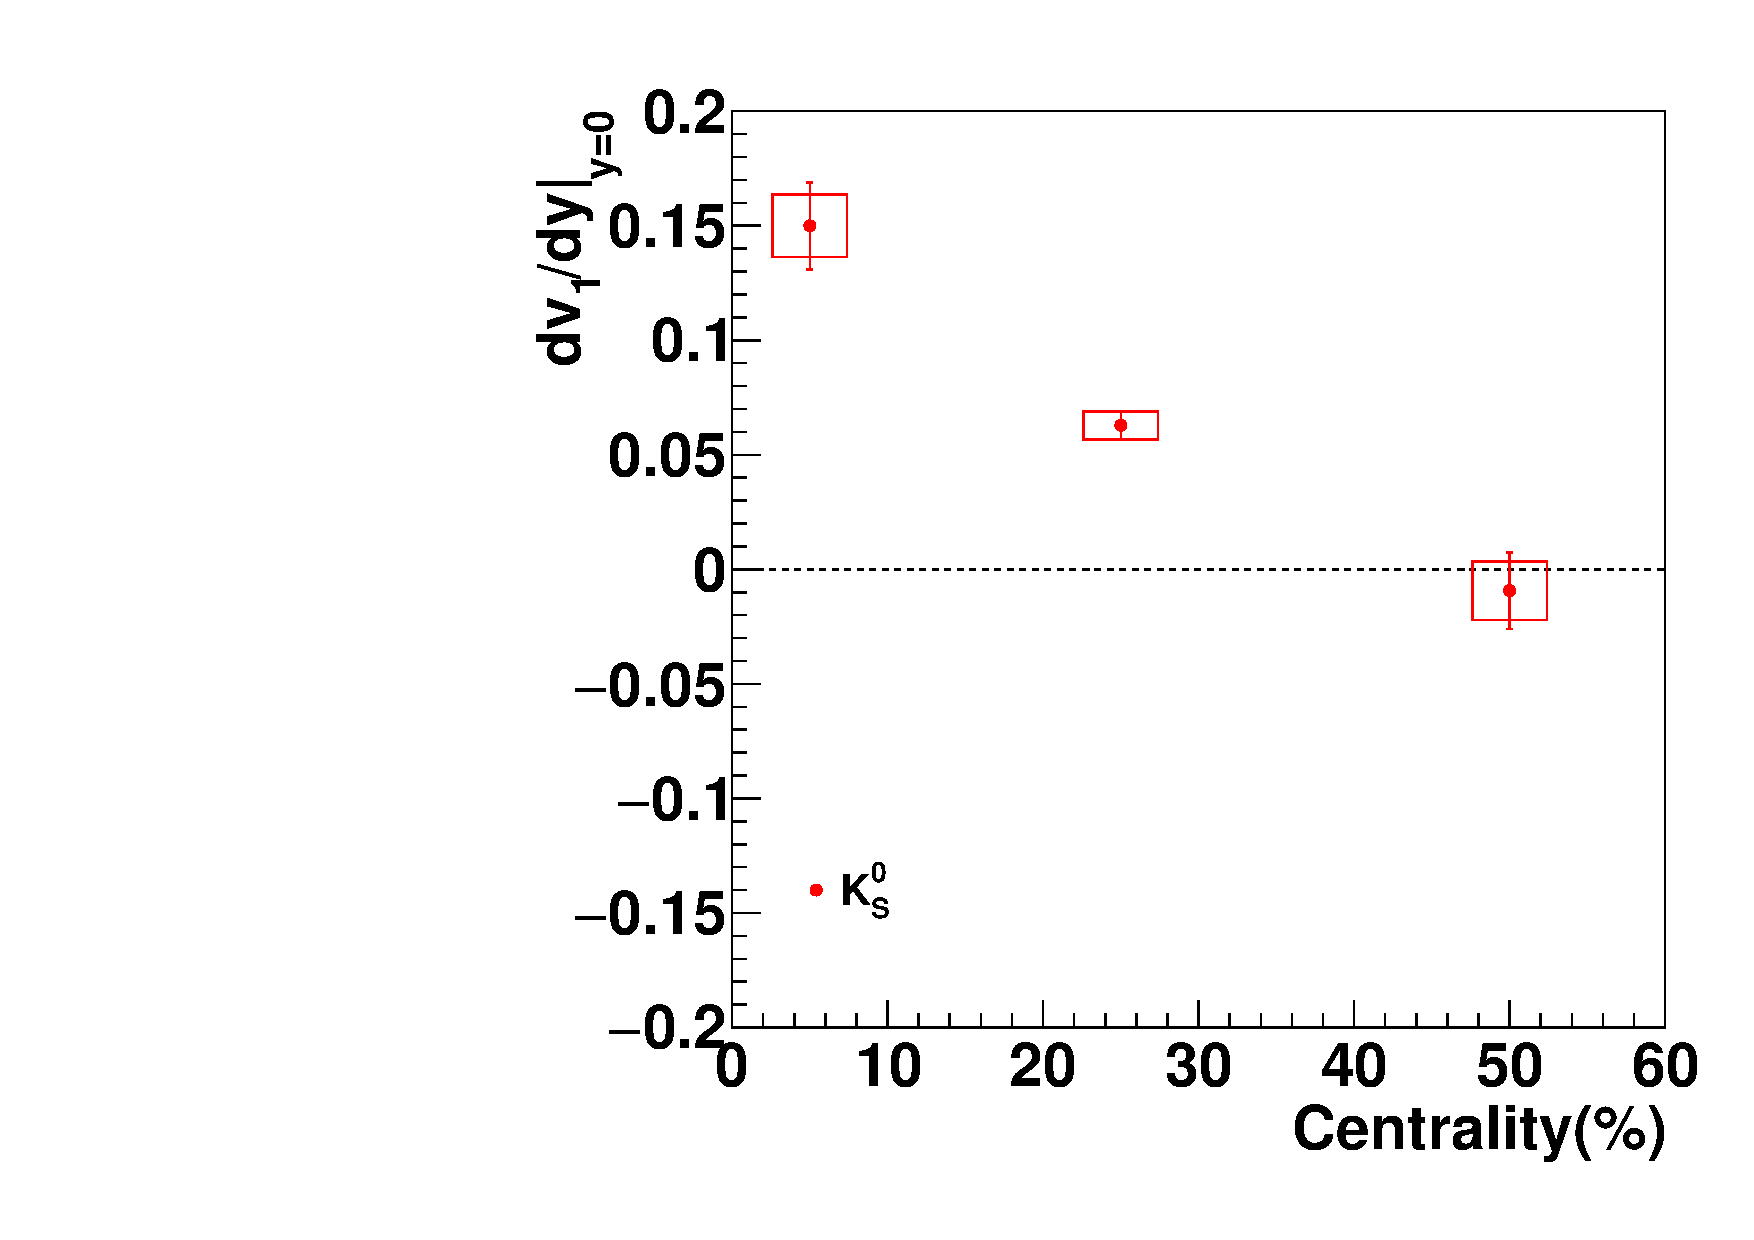
\includegraphics[width=0.49\linewidth]{chapterX/fig/ks_sys_vn.pdf}
\caption{$v_1$ as a function of rapidity(left) for $10-40\%$ centrality and  $dv_{1}/dy$ as a function of centrality(right) for $K^{0}_{S}$ at $\sqrt{s_{NN}}$ = 3 GeV.}
\label{ks_dv1dy_sys}
\end{figure}

\begin{figure}[h]
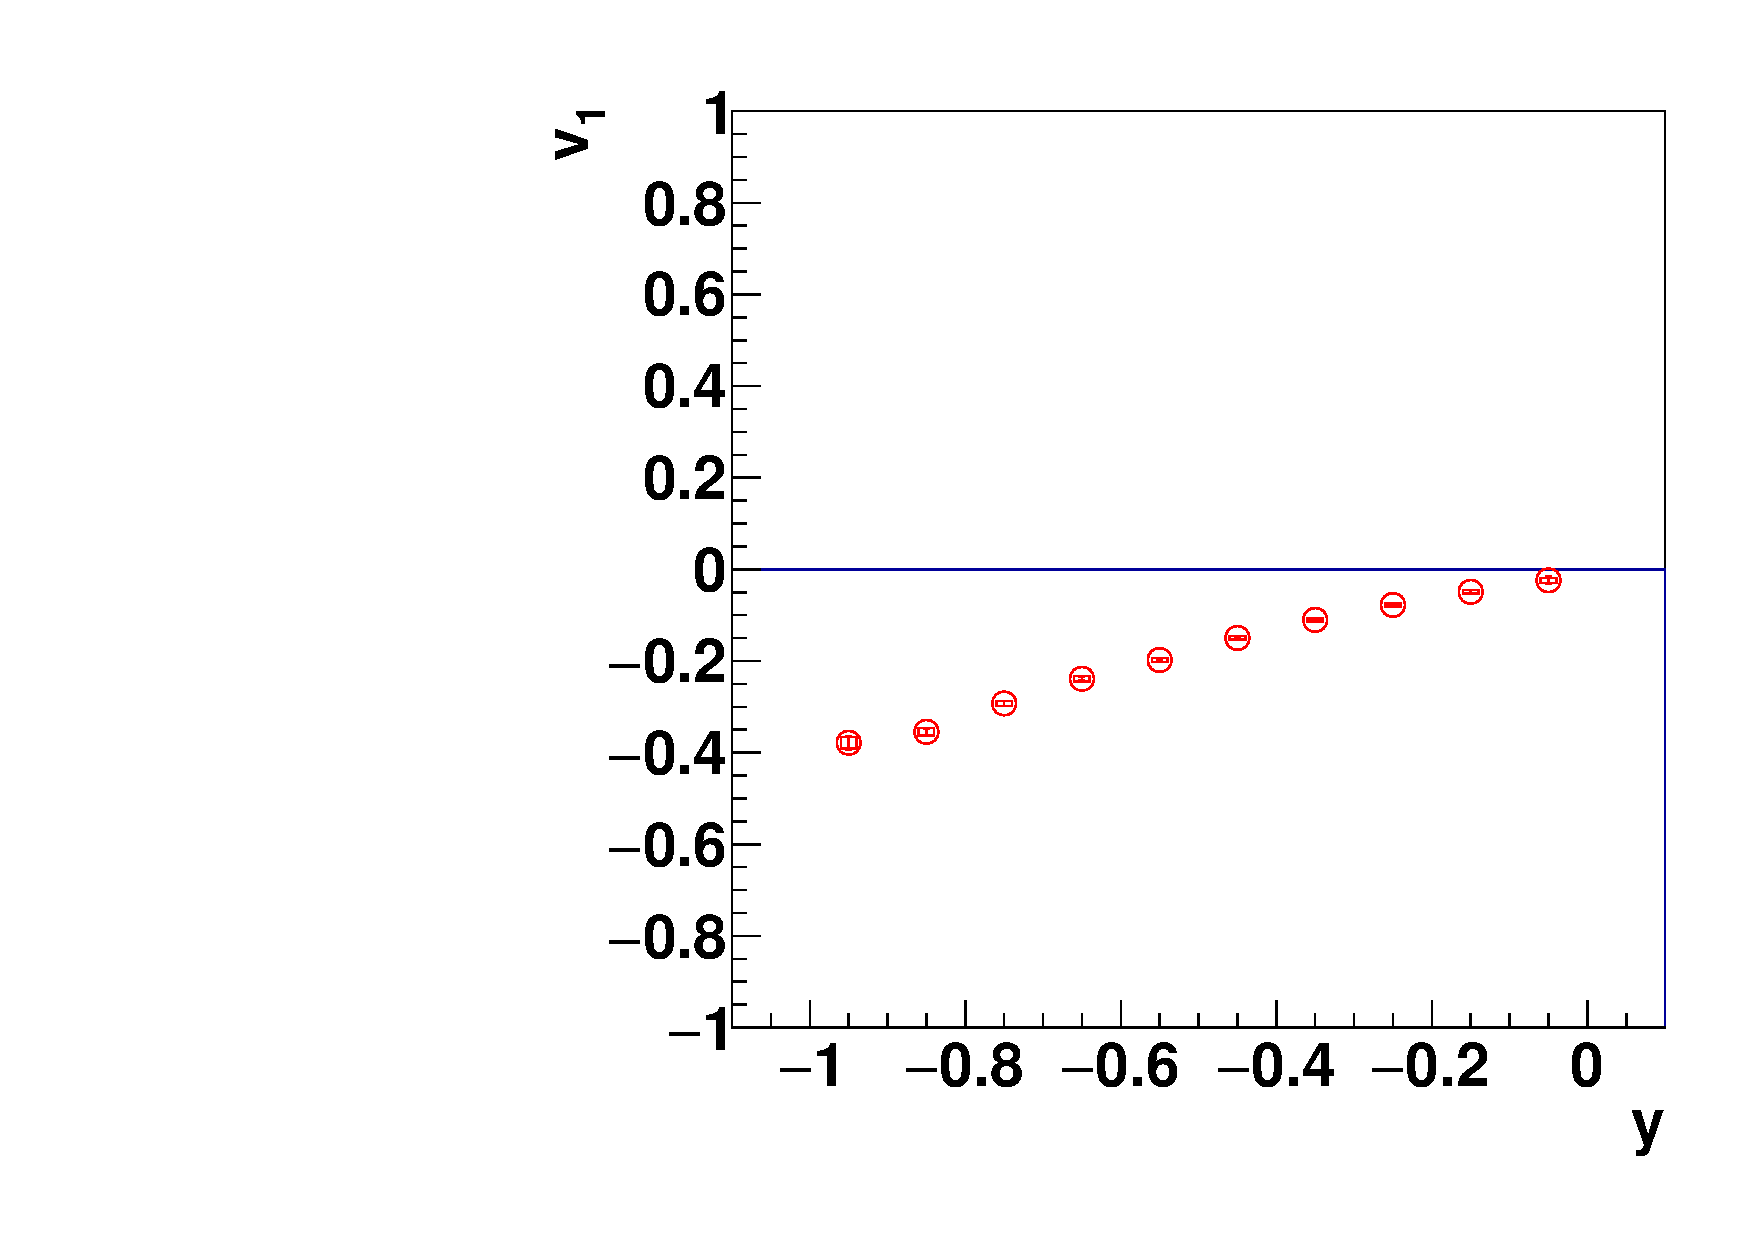
\includegraphics[width=0.49\linewidth]{chapterX/fig/ld_sys_v1.pdf}
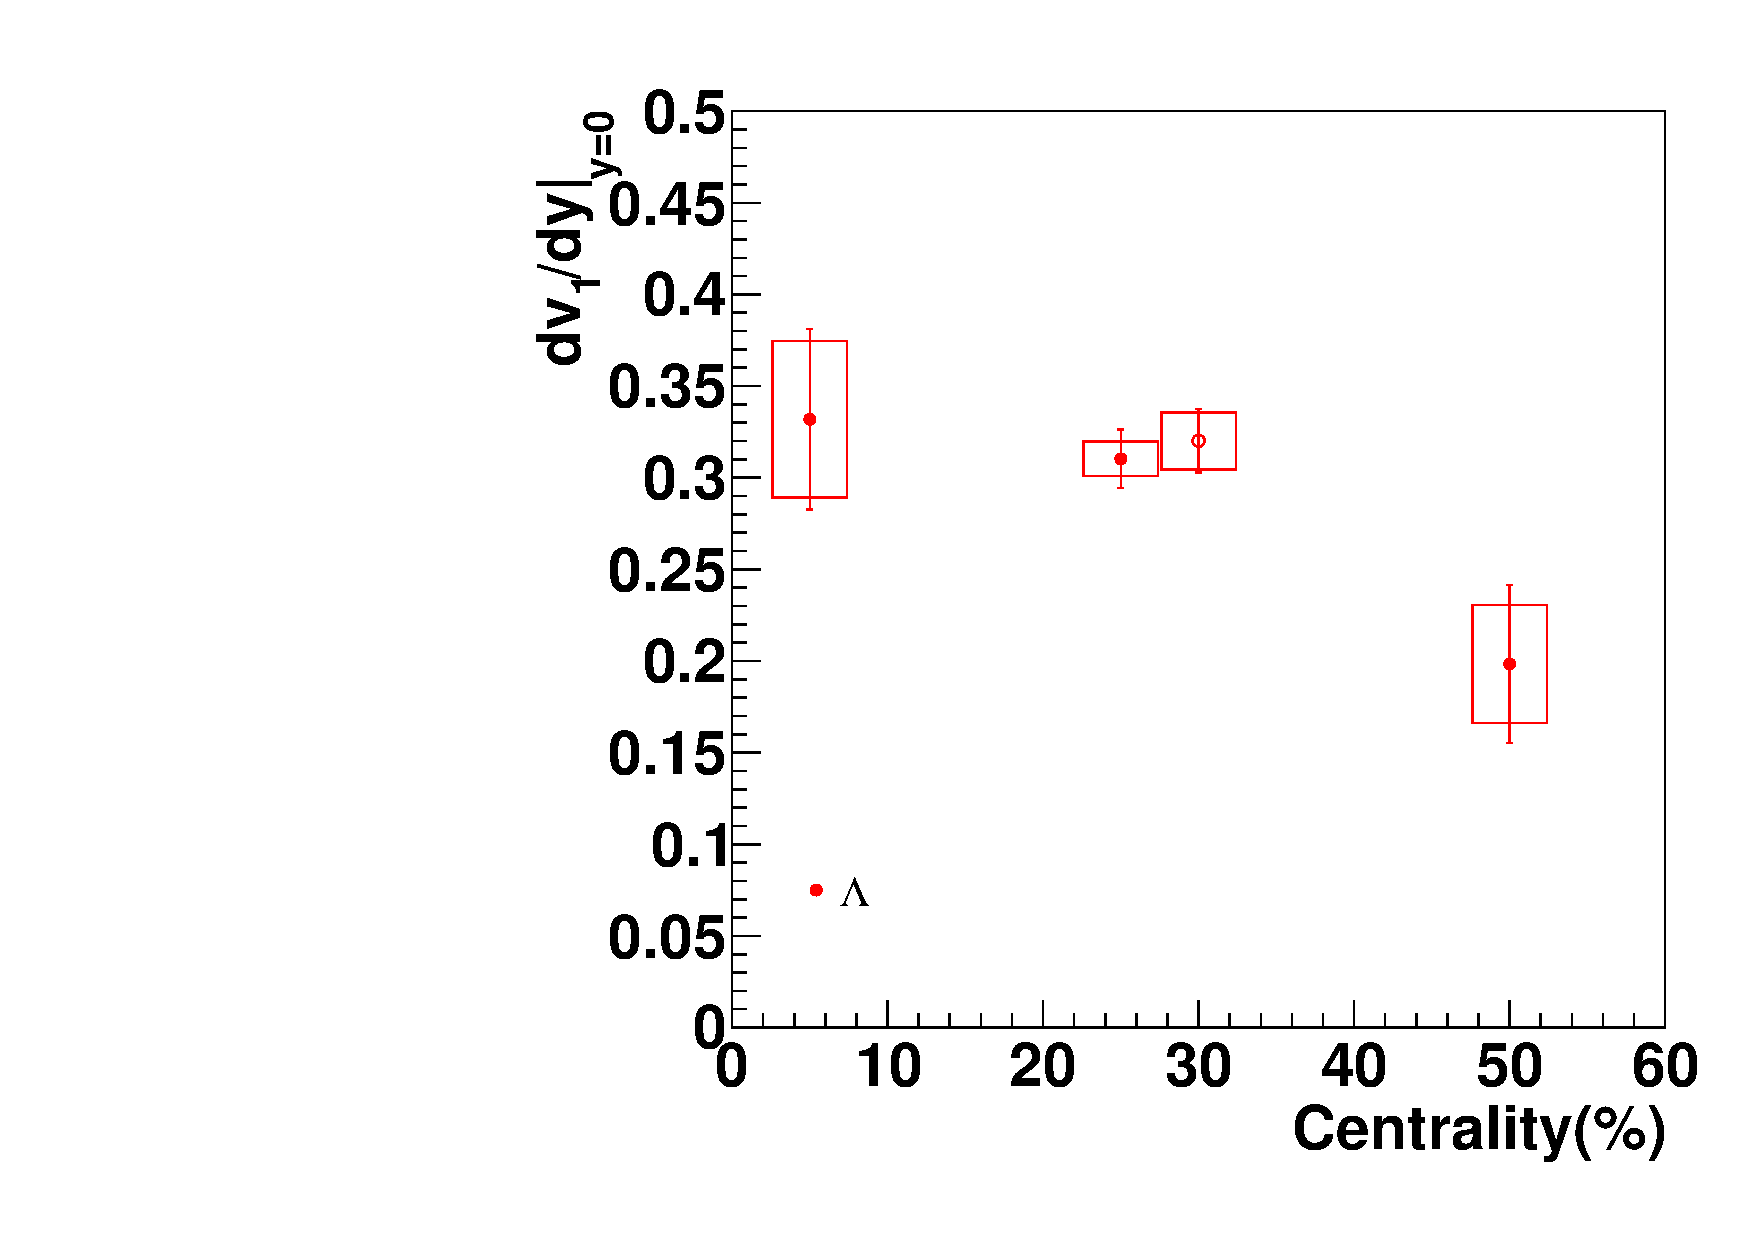
\includegraphics[width=0.49\linewidth]{chapterX/fig/ld_sys_vn.pdf}
\caption{$v_1$ as a function of rapidity(left) for $10-40\%$ centrality and  $dv_{1}/dy$ as a function of centrality(right) for $\Lambda$ at $\sqrt{s_{NN}}$ = 3 GeV.}
\label{lambda_dv1dy_sys}
\end{figure}


\subsubsection{$v_2$ results for $K^0_S$, $\Lambda$}

\begin{figure}[h]
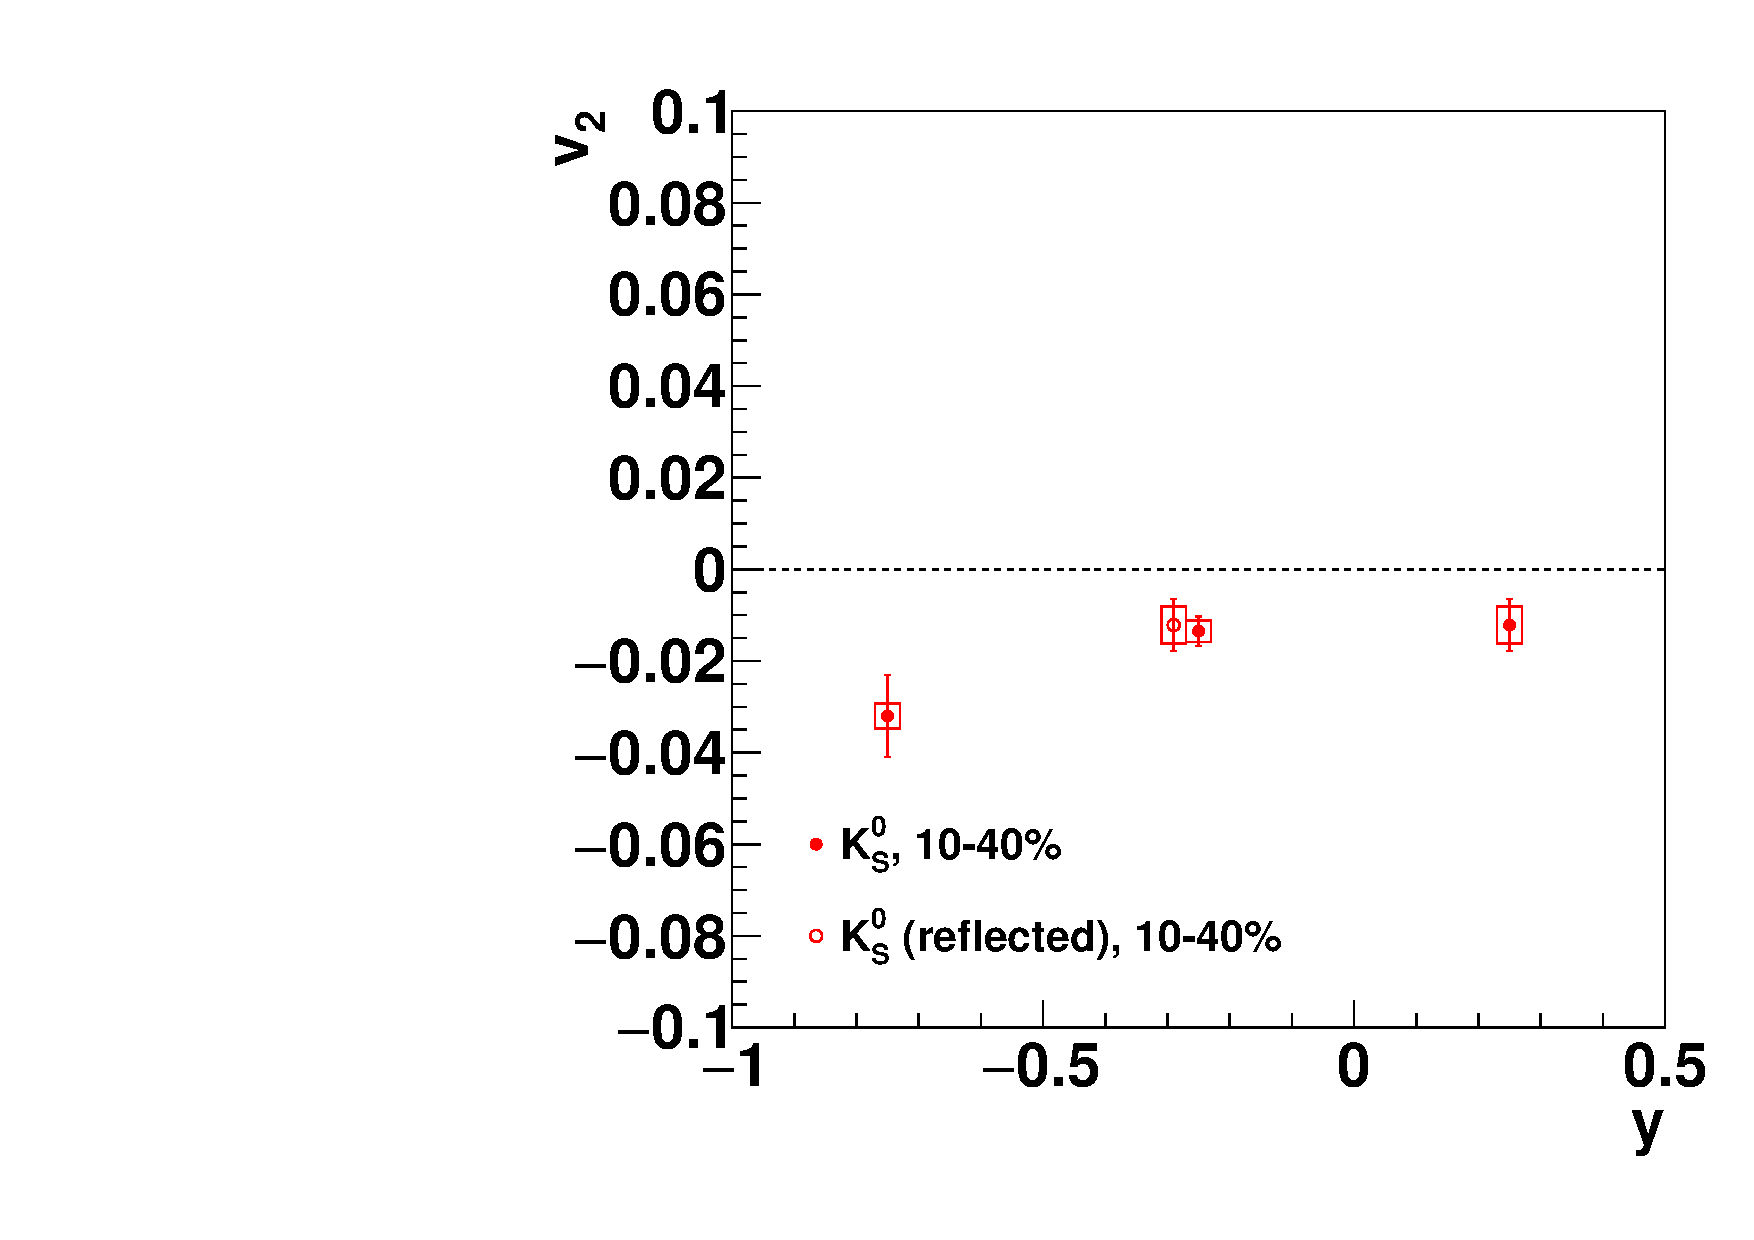
\includegraphics[width=0.49\linewidth]{chapterX/fig/ks_sys_v2.pdf}
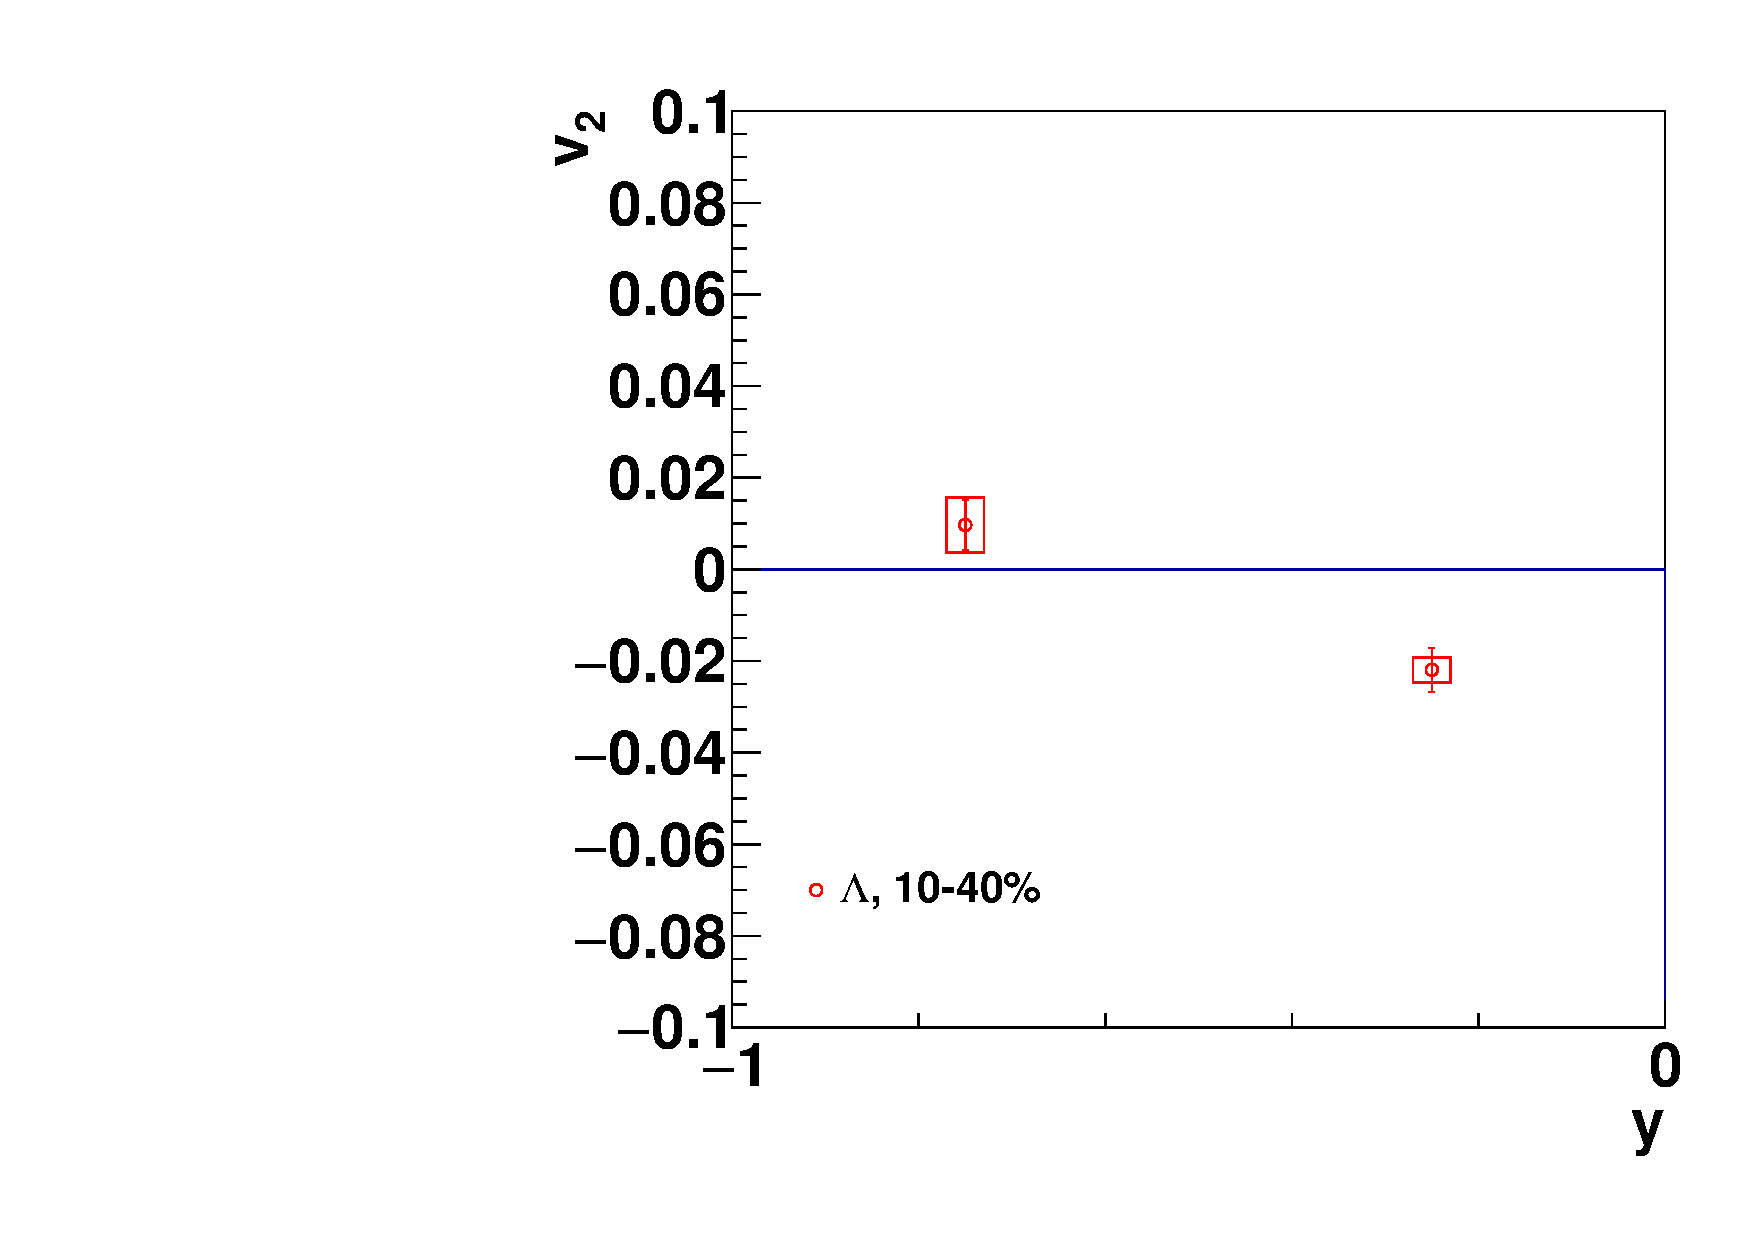
\includegraphics[width=0.49\linewidth]{chapterX/fig/ld_sys_v2.pdf}
\caption{$K^0_S$(left) and $\Lambda$(right) $v_2$ as a function of rapidity for $10-40\%$ centrality at $\sqrt{s_{NN}}$ = 3 GeV. For $K^0_S$, the forward rapidity is reflected to compare with the backward rapidity result.}
\label{ks_dv1dy_sys}
\end{figure}



\begin{figure}[h]
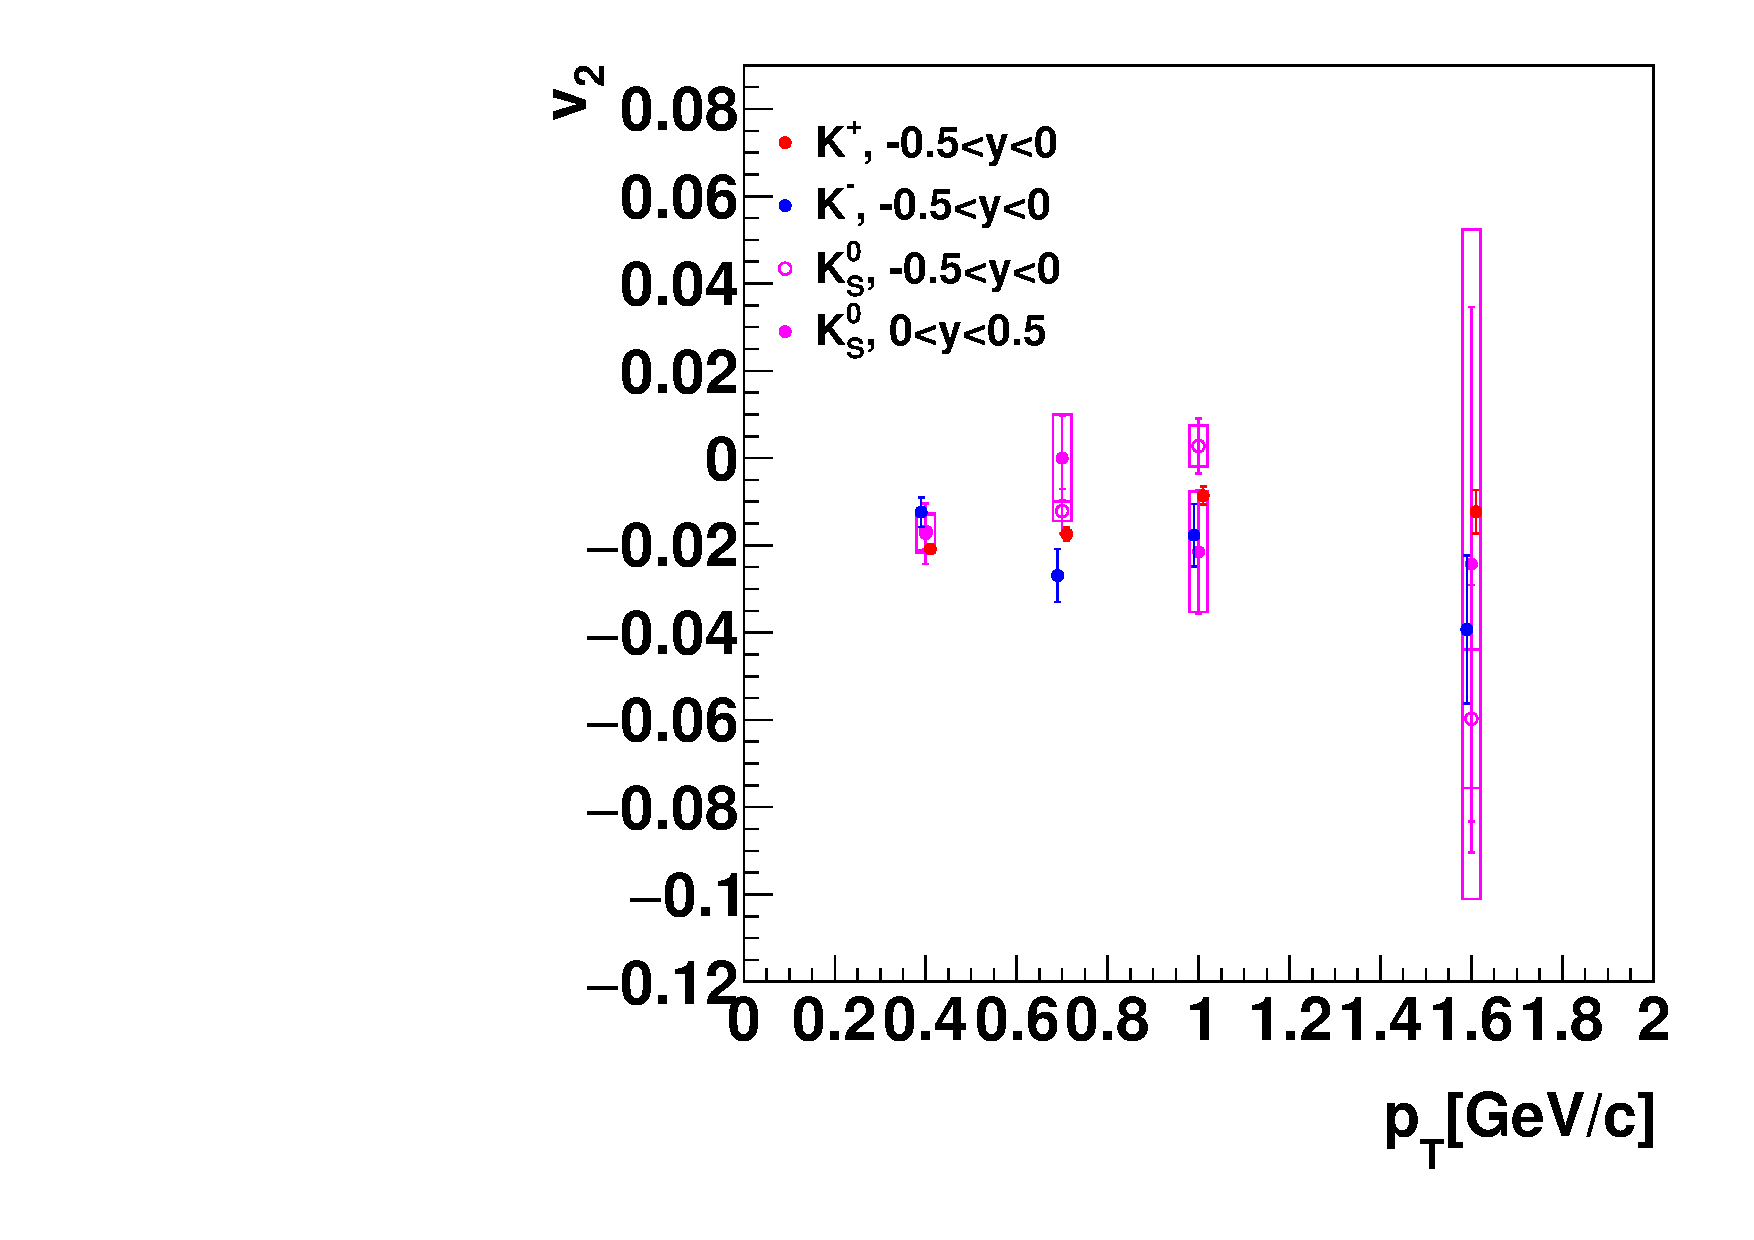
\includegraphics[width=0.32\linewidth]{chapterX/fig/q_v2_k_pt.pdf}
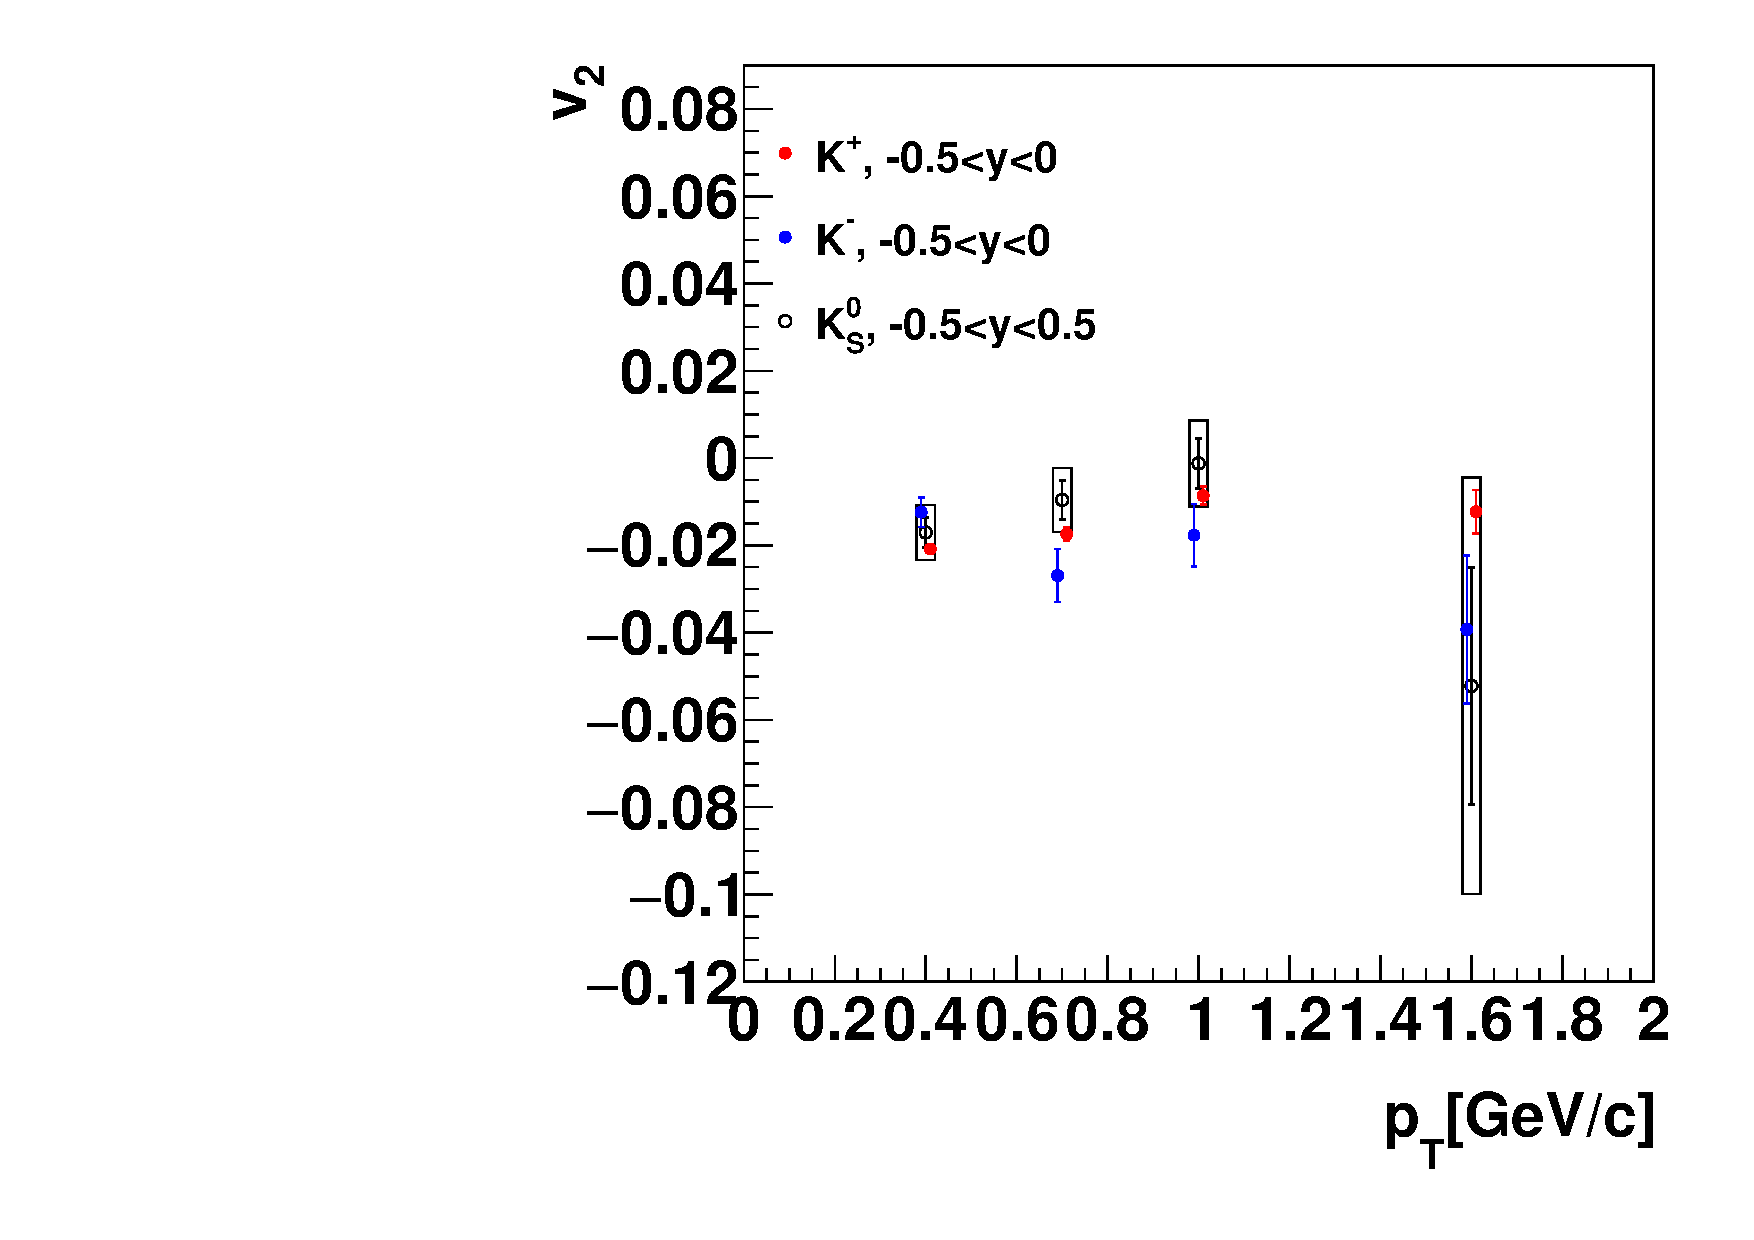
\includegraphics[width=0.32\linewidth]{chapterX/fig/q_v2_k_pt_check.pdf}
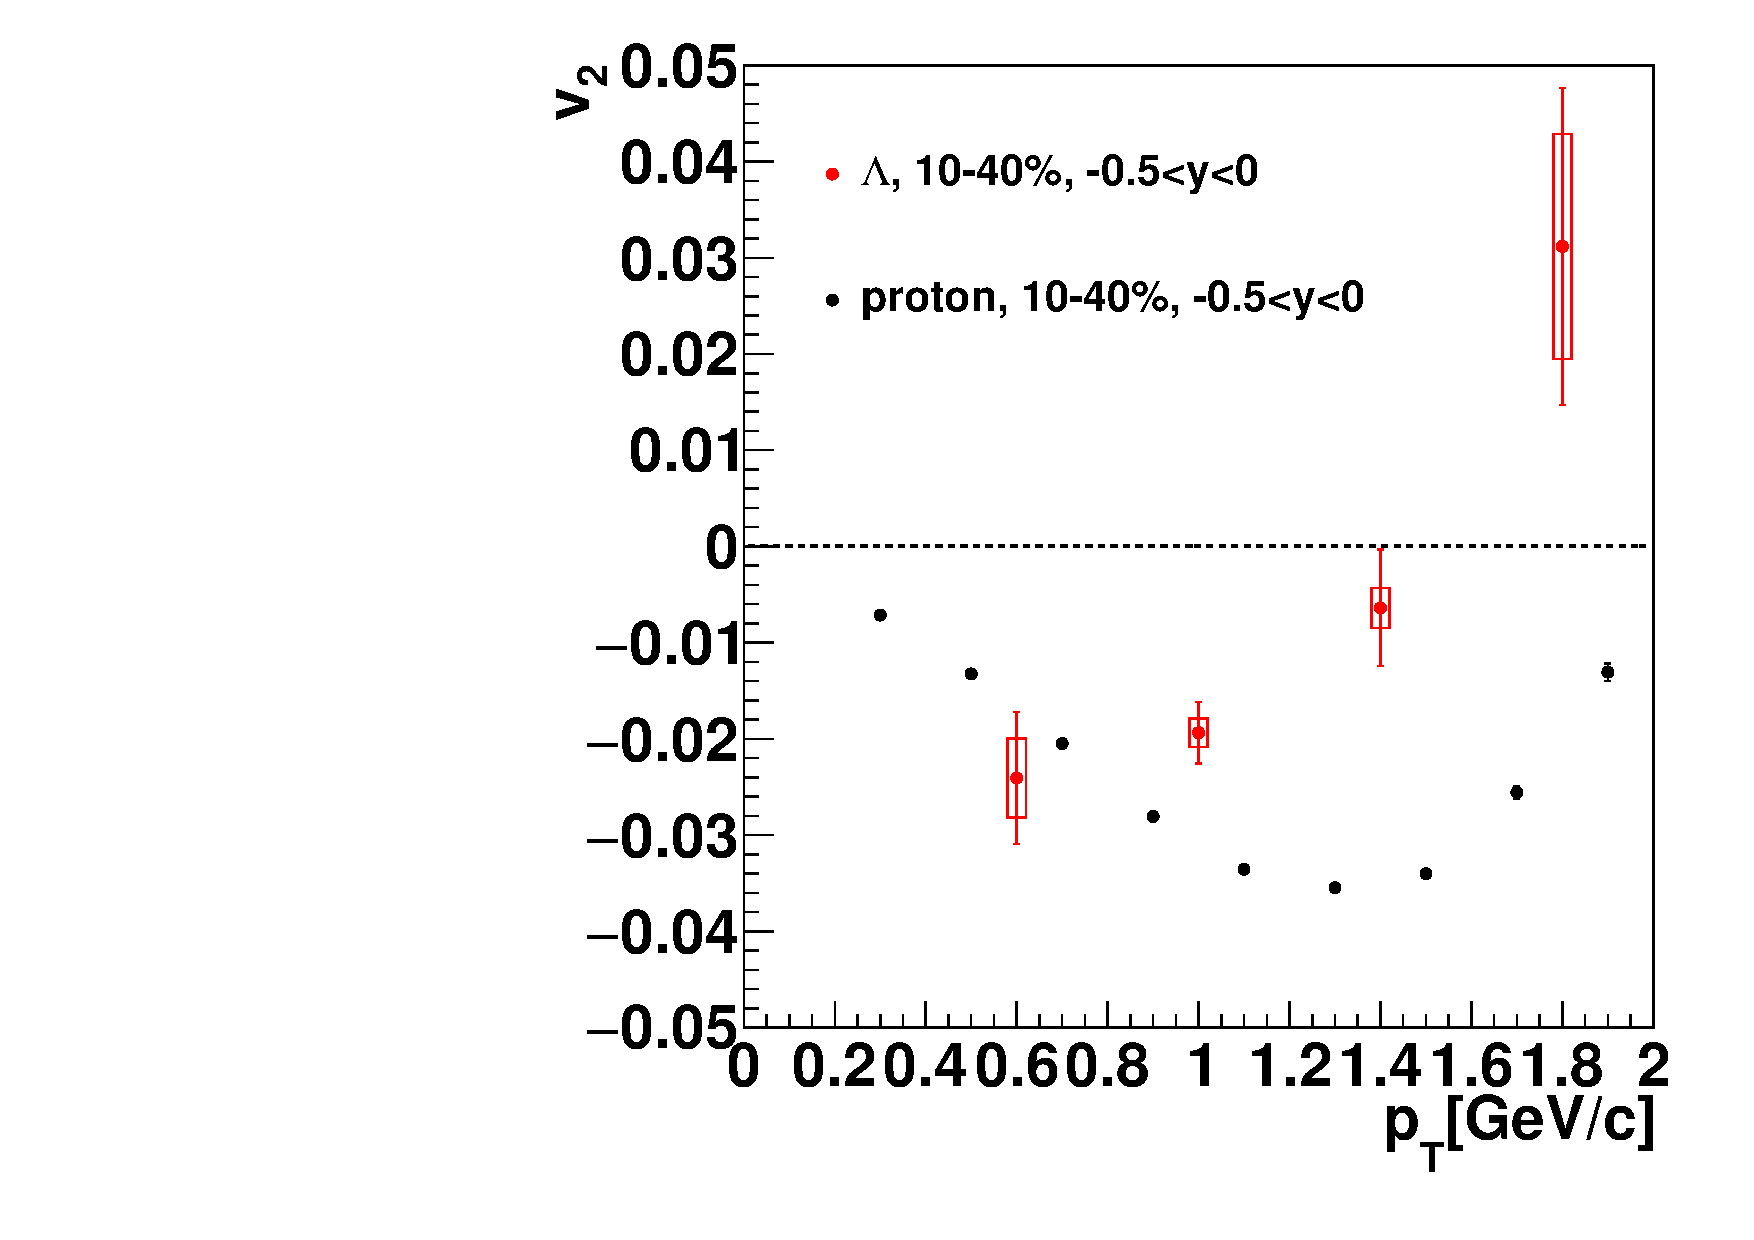
\includegraphics[width=0.32\linewidth]{chapterX/fig/data_v2_ld_pt.pdf}
\caption{$K^0_S$(left, middle) and $\Lambda$(right) $v_2$ as a function of $p_{T}$ in different rapidity ranges for $10-40\%$ centrality at $\sqrt{s_{NN}}$ = 3 GeV. The results are compared with protons and charged kaons.}
\label{ldks_dv2dpt}
\end{figure}


\begin{figure}[h]
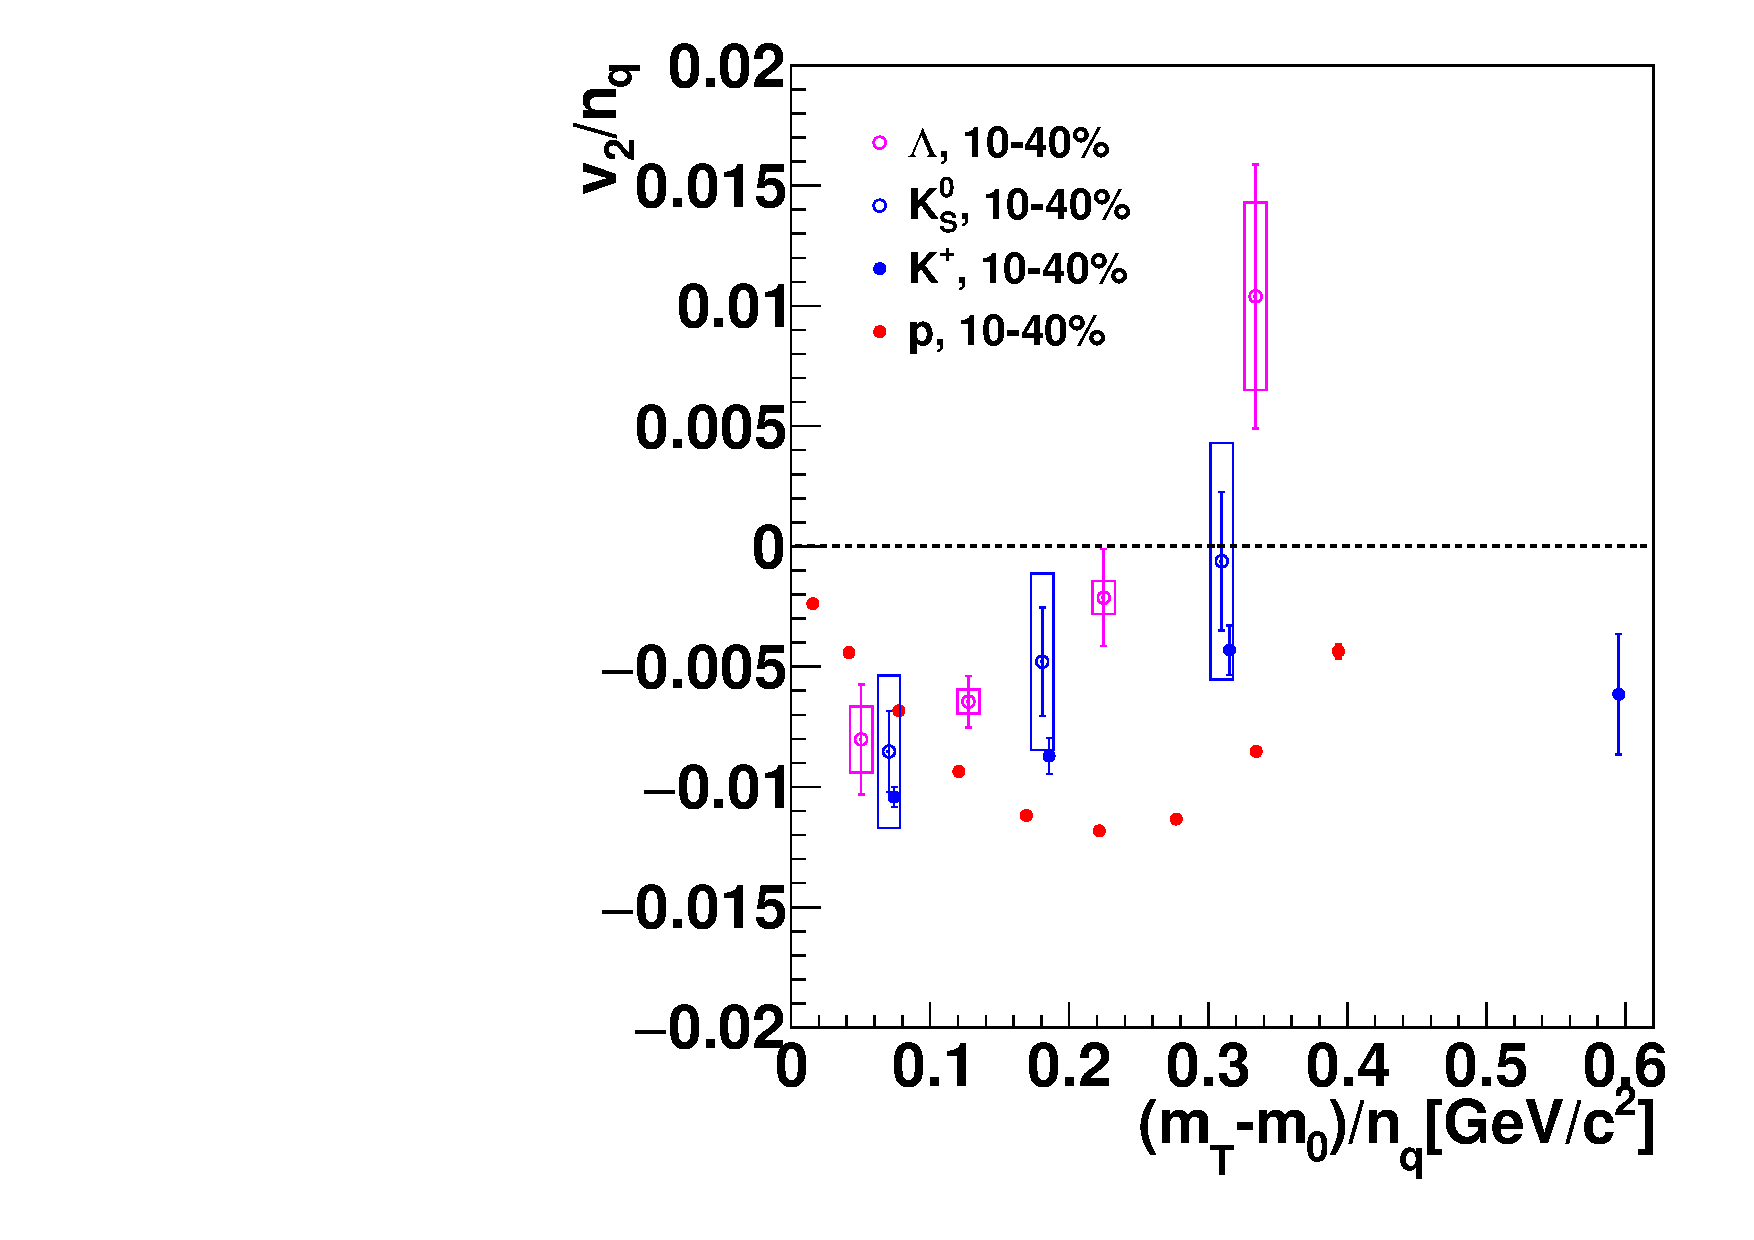
\includegraphics[width=0.80\linewidth]{chapterX/fig/data_v2_ld_ks_mt.pdf}
\caption{$K^0_S$ and $\Lambda$(right) $v_2/q$ as a function of $(m_{T}-m_{0})/n_{q}$ at mid-rapidity for $10-40\%$ centrality at $\sqrt{s_{NN}}$ = 3 GeV. The results are compared with protons and charged kaons.}
\label{ldks_dv2dmt}
\end{figure}
